% laden der Präambel mit Latexbefehlen/-klassen
% =============================================================================
% Dokumentklasse und Spracheinstellung
% =============================================================================
% für elektronische Veröffentlichung (Standard)
\documentclass[11pt,oneside,paper=A4,DIV=11,BCOR=0mm,abstract=true,headsepline,headings=normal,ngerman]{scrreprt}

\usepackage[ngerman]{babel}
\usepackage[utf8]{inputenc}
\usepackage[T1]{fontenc}

% =============================================================================
% Schriftart & Typographie
% =============================================================================
\usepackage{libertine}
\usepackage{libertinust1math}
\usepackage[auto]{microtype}
\usepackage[htt]{hyphenat}          % Silbentrennung in \texttt
\setlength{\emergencystretch}{3em}  % Notfall-Streckung bei langen Code-Snippets

% Verhindert "Schusterjungen" und "Hurenkinder" (einzelne Zeilen auf neuer Seite)
\clubpenalty = 10000
\widowpenalty = 10000
\displaywidowpenalty = 10000

% Floats auf Float-Seiten oben ausrichten statt vertikal zentrieren
\makeatletter
\setlength{\@fptop}{0pt}
\setlength{\@fpbot}{0pt plus 1fil}
\makeatother

% =============================================================================
% Mathe, Symbole, Einheiten
% =============================================================================
\usepackage{amsmath}
\usepackage{amsxtra}
\usepackage{eurosym}
\usepackage{siunitx}  
\sisetup{locale=DE}
\usepackage[version=4]{mhchem}
\usepackage{chemfig}

% =============================================================================
% Bilder, Tabellen, Quellcode
% =============================================================================
\usepackage{graphicx}
\setkeys{Gin}{width=\textwidth,height=0.45\textheight,keepaspectratio}
% Abbildung mit benutzerdefinierter Breite (Höhenlimit bleibt einheitlich)
\newcommand{\narrowfig}[2][0.8]{%
  \includegraphics[width=#1\textwidth,height=0.45\textheight,keepaspectratio]{#2}}
% Für gestapelte Subfigures: kleineres Höhenlimit damit beide passen
\newcommand{\stackedfig}[1]{%
  \includegraphics[width=\textwidth,height=0.35\textheight,keepaspectratio]{#1}}
\usepackage{float}
\usepackage{multirow,multicol,booktabs}
\usepackage{threeparttable}
\usepackage{longtable}
\usepackage{rotating}
\usepackage{pdflscape}  % Landscape-Seiten für Anhang-Tabelle
\usepackage{ltablex} % Kombination aus tabularx und longtable
\usepackage{subcaption}
\captionsetup[subtable]{position=top}
\usepackage{pdfpages}
\usepackage{listings}
\lstdefinelanguage{TypeScript}{
  keywords={break, case, catch, continue, debugger, default, delete, do, else,
    finally, for, function, if, in, instanceof, new, return, switch, this,
    throw, try, typeof, var, void, while, with, const, let, of, class,
    extends, import, export, from, interface, type, enum, implements,
    abstract, as, async, await, declare, keyof, namespace, readonly,
    undefined, null, true, false, any, string, number, boolean, never, void,
    object, symbol, bigint, unknown},
  sensitive=true,
  comment=[l]{//},
  morecomment=[s]{/*}{*/},
  morestring=[b]',
  morestring=[b]",
  morestring=[b]`,
}
\usepackage{blindtext}
\usepackage{csquotes}

% Darstellung von URL (wird von hyperref später erweitert)
\usepackage{url}
\urlstyle{same}

% \code{...}: Inline-Code mit Zeilenumbruch an Sonderzeichen
% Für reine Texte ohne LaTeX-Befehle; \texttt bleibt für Argumente mit \, etc.
\newcommand{\code}[1]{\texttt{\nolinkurl{#1}}}

% Fussnoten, auch für Tabellen
\usepackage{footnote}
\makesavenoteenv{tabular} 

% =============================================================================
% Literaturverzeichnis (BibLaTeX)
% =============================================================================
\usepackage[
backend=biber,
style=numeric,
sorting=none,
citestyle=numeric-comp,
maxbibnames=10,
giveninits=true,
]{biblatex}

\renewcommand*{\labelnamepunct}{\addcolon\addspace}

% Pfad zur .bib Datei
\addbibresource{literatur/literaturdatenbank.bib}

% =============================================================================
% Nomenklatur / Abkürzungsverzeichnis
% =============================================================================
\usepackage[intoc, german]{nomencl}
\makenomenclature

\RedeclareSectionCommand[tocbeforeskip=0.5em plus 0.3em]{chapter}
\renewcommand{\nomname}{Abkürzungs- und Symbolverzeichnis}
\setlength{\nomitemsep}{-\parsep}
\newlength{\nomgroupstartsep}
\setlength{\nomgroupstartsep}{18pt}

\newcommand{\nomenclheader}[1]{\item[\hspace*{-\itemindent}\itshape#1]{\ } \vspace{6pt}\par}

\renewcommand\nomgroup[1]{%
	\itemsep\nomgroupstartsep
	\ifstrequal{#1}{A}{\nomenclheader{Abkürzungen}}{%
		\ifstrequal{#1}{E}{\newpage\nomenclheader{Lateinische Symbole}}{%
			\ifstrequal{#1}{G}{\nomenclheader{Griechische Symbole}}{%
				\ifstrequal{#1}{O}{\nomenclheader{Operatoren}}{%
					\ifstrequal{#1}{X}{\nomenclheader{Tiefgestelle Indizes}}{%
						\ifstrequal{#1}{Y}{\nomenclheader{Hochgestelle Indizes}}{}}}}}}%
	\itemsep\nomitemsep
}

% =============================================================================
% Fußnoten-Design
% =============================================================================
% Linksbündige Fußnotenmarkierungen
\deffootnote{1.5em}{1em}{%
	\makebox[1.5em][l]{\thefootnotemark}%
}

% Fußnoten nicht über Seiten umbrechen
\interfootnotelinepenalty=10000

% =============================================================================
% Beschriftungen (Captions) und KOMA-Fonts
% =============================================================================
\addtokomafont{caption}{\small}
\setkomafont{captionlabel}{\sffamily\bfseries}
\setkomafont{author}{\large}
\setkomafont{date}{\large}
\setkomafont{publishers}{\large}
\setkomafont{dedication}{\normalsize}
\addtokomafont{dedication}{\raggedright}

\renewcaptionname{ngerman}{\figurename}{Abb.}
\renewcaptionname{ngerman}{\tablename}{Tab.} 

% Eigene Tabellenumgebungen
\newenvironment{tabular10}{%
	\fontsize{10}{12}\selectfont\tabular
}{%
	\endtabular
}

\newenvironment{tabular7}{%
	\fontsize{7}{12}\selectfont\tabular
}{%
	\endtabular
}

% =============================================================================
% Datenimport & Hyperref (Muss fast am Ende stehen!)
% =============================================================================
%\def\VARtyp{Bachelorarbeit}
\def\VARtyp{Bachelorarbeit}

\def\VARtitel{Performance- und Ressourcenanalyse von
	React und Svelte bei steigender UI-Dichte und
	Update-Frequenz}


\def\VARname{Jonas Öhler}

\def\VARmatrikelnummer{44338}

\def\VARstudiengang{Medieninformatik}

\def\VARhochschule{Hochschule der Medien Stuttgart}

\def\VARabgabedatum{20.07.2026}

\def\VARabschlussbezeichnung{Bachelor of Science}

\def\VARerstbetreuung{Prof. Dr. Simon Wiest}
\def\VARzweitbetreuung{Prof. Dr. Tobias Jordine}

%wenn keine externe Arbeit, dann extern auf false setzen



\usepackage[
pdftitle={\VARtitel},
pdfsubject={\VARtyp},
pdfauthor={\VARname},
pdfkeywords={},  
hidelinks,      % Links im PDF nicht umranden
breaklinks=true % Zeilenumbruch bei langen URLs erlauben
]{hyperref}

% Cleveref als Abschluss für intelligente Querverweise
\usepackage[german]{cleveref}

% Umbruchzeichen für \code{...} nach hyperref erweitern
\expandafter\def\expandafter\UrlBreaks\expandafter{\UrlBreaks%
  \do\(\do\)\do\,\do\;\do\_\do\=\do\.\do\/\do\@\do\'}

\begin{document}
% globale Einstellung für Quellcodedarstellung mit listings
\lstset{basicstyle=\scriptsize\ttfamily,language={[LaTeX]TeX}}

% Seitennummerierung römisch
\pagenumbering{roman}

% Titelseiten
% Deckblatt

\begin{center}
	\begin{Large}
		\textbf{\VARtyp}\\
		im Studiengang {\VARstudiengang}
	\end{Large}
	\vskip 1.5cm
	\begin{Huge}
		{\VARtitel}
	\end{Huge}
	\vskip 1.5cm
	\begin{Large}
		vorgelegt von \\
		\vskip 1.5cm
		
		\textbf {\VARname}\\
			Matrikelnummer: {\VARmatrikelnummer}
		
		\vskip 1.5cm
		%\begin{center}
		%\includegraphics{Pictures/HdM-Logo.pdf}
		%\end{center}
		an der {\VARhochschule} am \\
		{\VARabgabedatum} \\
		zur Erlangung des akademischen Grades eines {\VARabschlussbezeichnung}
		
		\vskip 2cm
		
		\begin{tabular}{ll}
			Erstprüfer: & {\VARerstbetreuung}\\ 
			Zweitprüfer: & {\VARzweitbetreuung}
		\end{tabular}
		%\vskip 1.5cm
		%
		%Bearbeitungszeitraum: <Tag. Monat Jahr> bis <Tag. Monat Jahr>\fxnote{Abgabedatum anpassen}
		
	\end{Large}
	
\end{center}
\vfill


%Eigenständigkeitserklärung
\cleardoubleemptypage
\thispagestyle{empty}
\subsection*{Ehrenwörtliche Erklärung}
Hiermit versichere ich, \VARname, ehrenwörtlich, dass ich die vorliegende
Bachelorarbeit mit dem Titel: „\VARtitel“ selbstständig und ohne fremde Hilfe verfasst und keine anderen als die angegebenen
Hilfsmittel benutzt habe. Die Stellen der Arbeit, die dem Wortlaut oder dem Sinn nach anderen Werken
entnommen wurden, sind in jedem Fall unter Angabe der Quelle kenntlich gemacht. Ebenso sind alle
Stellen, die mit Hilfe eines KI-basierten Schreibwerkzeugs erstellt oder überarbeitet wurden, kenntlich
gemacht. Die Arbeit ist noch nicht veröffentlicht oder in anderer Form als Prüfungsleistung vorgelegt
worden. \\  
Ich habe die Bedeutung der ehrenwörtlichen Versicherung und die prüfungsrechtlichen Folgen
(§ 24 Abs. 2 Bachelor-SPO, § 23 Abs. 2 Master-SPO (Vollzeit)) einer unrichtigen oder
Mai 2023 Prüfungsverwaltung 6
unvollständigen ehrenwörtlichen Versicherung zur Kenntnis genommen

\vspace{4\baselineskip}

\begin{tabular}{lp{2em}l}
	\hspace{5cm}   && \hspace{4cm} \\
	\cline{1-1}\cline{3-3}
	Ort, Datum     && Unterschrift
\end{tabular} 



%Zusammenfassung/Abstract
%\cleardoubleemptypage
\begin{abstract}
Reaktionsfähige Benutzeroberflächen sind in datenintensiven Echtzeit-Anwendungen wie Monitoring-Dashboards ein zentrales Qualitätsmerkmal. React~19 und Svelte~5 verfolgen dabei grundlegend unterschiedliche Architekturansätze: React~19 kombiniert ein Virtual-DOM-basiertes Laufzeitmodell mit einem Compiler zur automatischen Memoisierung, während Svelte~5 compilerbasierte feingranulare Reaktivität einsetzt. Bestehende Vergleichsstudien basieren jedoch überwiegend auf älteren Framework-Versionen und untersuchen vorwiegend isolierte Operationen; empirische Daten unter kombinierter Dauerlast aus steigender UI-Dichte und hoher Update-Frequenz fehlen bislang. Diese Arbeit untersucht, wie sich React~19 und Svelte~5 hinsichtlich Interaktionslatenz (INP), Scripting-Aufwand und Speicherverbrauch unter kombiniert steigender UI-Dichte und Update-Frequenz unterscheiden und ab welcher Last-Kombination \textit{Long Tasks} den Main Thread dauerhaft blockieren. Dazu wurden in einem automatisierten Benchmark (Playwright, Chrome DevTools Protocol) 1920 Messläufe über acht UI-Dichtestufen ($n \in \{100 \ldots 10\,000\}$) und vier Update-Frequenzen (10 bis 62\,Hz) durchgeführt. Als Metriken dienten INP, Scripting-Aufwand pro Tick, JS-Heap-Delta sowie Long-Task-Zähler. Die Ergebnisse zeigen, dass kein Framework uneingeschränkt überlegen ist. Bei hoher UI-Dichte liefert Svelte~5 in der Mehrzahl der Szenarien geringeren Scripting-Aufwand und niedrigere INP-Werte; zudem liegt Sveltes \textit{Tipping Point} bei höheren $n$-Werten. Über alle Dichtestufen weist Svelte~5 zudem einen 2,8- bis 6,4-fach geringeren Heap-Verbrauch auf. Allerdings erzielt React~19 bei moderater UI-Dichte und hoher Update-Frequenz durch kooperatives Yielding der Fiber-Engine niedrigere INP-Werte. Unter Extremlast ($n = 10\,000$, 62\,Hz) kehrt sich das Long-Task-Verhältnis um: Svelte erzeugt dort mehr \textit{Long Tasks} als React. Für die Praxis ergibt sich: Svelte~5 ist bei hoher UI-Dichte und in speicherkritischen Umgebungen vorzuziehen; React~19 kann bei moderater Dichte und hoher Update-Frequenz die bessere Wahl sein.
\end{abstract}

%\cleardoubleemptypage
\renewcommand\abstractname{Abstract}
\begin{abstract}
Responsive user interfaces are a central quality criterion in
data-intensive real-time applications such as monitoring dashboards.
React~19 and Svelte~5 pursue fundamentally different architectural
approaches: React~19 combines a virtual DOM-based runtime model with
a compiler for automatic memoization, while Svelte~5 employs
compiler-based fine-grained reactivity. However, existing comparison
studies are predominantly based on older framework versions and
examine primarily isolated operations; empirical data under combined
sustained load from increasing UI density and high update frequency
are lacking. This work investigates how React~19 and Svelte~5 differ
with respect to interaction latency (INP), scripting effort, and
memory consumption under combined increasing UI density and update
frequency, and at which load combination \textit{Long Tasks} persistently
block the main thread. To this end, 1920 measurement runs were
conducted in an automated benchmark (Playwright, Chrome DevTools
Protocol) across eight UI density levels ($n \in \{100 \ldots
10\,000\}$) and four update frequencies (10 to 62\,Hz). The metrics
used were INP, scripting effort per tick, JS heap delta, and long
task count. The results show that neither framework is universally
superior. At high UI density, Svelte~5 delivers lower scripting
effort and lower INP values in the majority of scenarios; Svelte's
\textit{tipping point} additionally lies at higher $n$ values. Across all
density levels, Svelte~5 additionally exhibits a 2.8- to 6.4-fold lower heap
consumption. However, React~19 achieves lower INP values at moderate
UI density and high update frequency through cooperative yielding of
the Fiber engine. Under extreme load ($n = 10\,000$, 62\,Hz), the long
task ratio reverses: Svelte produces more \textit{long tasks} than React. In practice: Svelte~5
is preferable at high UI density and in memory-constrained
environments; React~19 may be the better choice at moderate density
and high update frequency.
\end{abstract}

\cleardoubleemptypage

% Inhaltsverzeichnis
% Zeigt Kapitel (1) und Abschnitte (2) an.
\setcounter{tocdepth}{2}
\tableofcontents

\cleardoubleemptypage

% Seitennummerierung zurücksetzen und arabisch für den Hauptteil
\pagestyle{headings}
\pagenumbering{arabic}
\setcounter{page}{1}

% Beginn der Kapitel (\include nutzt automatisch \clearpage)
\chapter{Einleitung}
\label{ch:einleitung}

\section{Motivation}
\label{s:motivation}

Die Reaktionsfähigkeit einer Webanwendung ist ein zentraler Bestandteil der Nutzererfahrung: Verzögerungen bei der Eingabeverarbeitung sowie ruckelnde Animationen beeinträchtigen unmittelbar die wahrgenommene Qualität der Benutzeroberfläche \cite{mdn-perceived-performance-2026}. Mit der Einführung der Core Web Vitals hat Google diesen Zusammenhang messbar gemacht. Die Metrik \textit{Interaction to Next Paint} (INP) misst über die gesamte Nutzungsdauer hinweg, wie schnell eine Webseite auf Nutzereingaben reagiert \cite{web.dev_inp_2025}. Besonders herausfordernd sind datenintensive Echtzeit-Anwendungen wie Monitoring-Dashboards oder interaktive Visualisierungen. In solchen Systemen führen kontinuierliche Datenströme dazu, dass große Teile der Benutzeroberfläche in hoher Frequenz aktualisiert werden \cite{furrer-livedashboard-2018}. Jede dieser Operationen belastet den sogenannten \textit{Main Thread} des Browsers, auf dem sowohl die Framework-Logik als auch die Rendering-Pipeline ausgeführt werden \cite{mdn_mthread_2025}. Überschreitet die Verarbeitungszeit pro Frame das verfügbare Zeitfenster von etwa $16{,}7\,\text{ms}$, entstehen wahrnehmbare Stockungen (\textit{Jank}) und eine erhöhte Interaktionslatenz \cite{web.dev_rendering_2023}. Die Wahl des UI-Frameworks bestimmt dabei entscheidend, wie effizient dieses begrenzte Zeitbudget genutzt wird.

\section{Ausgangssituation und Forschungslücke}
\label{s:ausgangssituation}

React und Svelte basieren auf grundsätzlich unterschiedlichen Architekturansätzen. React setzt auf ein Virtual-DOM-basiertes Laufzeitmodell, bei dem Zustandsänderungen zur Laufzeit durch einen Differenzierungsalgorithmus (\textit{Reconciliation}) in DOM-Operationen umgewandelt werden \cite{kumar-fluentreact-2024}. Svelte setzt stattdessen auf einen Compiler, der den Komponentencode bereits zur Kompilierzeit in direkten DOM-Manipulationscode übersetzt. Dadurch werden zur Laufzeit weder ein Virtual DOM noch ein Differenzierungsverfahren benötigt \cite{svelte_vdom-2018}. React 19 und Svelte 5 haben in beiden Frameworks neue Architekturkonzepte eingeführt. React 19 integriert einen Compiler, der die bisher manuelle Memoisierung von Komponenten automatisiert \cite{react_compiler_2025}. Svelte 5 führt mit sogenannten \textit{Runes} ein signalbasiertes Reaktivitätsmodell ein, bei dem zur Laufzeit automatisch erkannt wird, welche DOM-Knoten bei einer Zustandsänderung aktualisiert werden müssen \cite{svelte_runes_2023}. Da beide Neuerungen das jeweilige Reaktivitätsmodell grundlegend verändern, lassen sich frühere Leistungsmessungen nicht mehr auf die aktuellen Versionen übertragen. Diese Entwicklung wird in der bisherigen Forschungsliteratur nicht berücksichtigt. Vergleichende Leistungsstudien basieren überwiegend auf älteren Framework-Versionen wie Svelte 3 und React 16 oder 18 \cite{levlin-dom-benchmark-2020, putra-performance-2025, ollila-rendering_performance-2022}. Zudem untersuchen bestehende Benchmarks nur isolierte Operationen wie das initiale Rendern oder das Einfügen von Listeneinträgen unter kontrollierten Bedingungen \cite{krause-benchmark-2026}. Ungeklärt ist bislang, wie beide Frameworks unter einer kombinierten Dauerlast aus hoher UI-Dichte und hoher Update-Frequenz reagieren und ab welchem Punkt diese Last den Main Thread durch \textit{Long Tasks} dauerhaft blockiert (vgl.\ \cref{s:research-gap}).

\section{Zielsetzung und Forschungsfrage}
\label{s:zielsetzung}

Ziel dieser Arbeit ist es, den \textit{Tipping Point} beider Frameworks empirisch zu bestimmen: den Übergang, an dem die kombinierte Last aus UI-Dichte~$n$ (Anzahl gleichzeitig gerenderter Komponenten) und Update-Frequenz~$f$ den Main Thread durch Long Tasks \cite{w3c_longtasks_2026} dauerhaft blockiert und die Interaktionslatenz messbar verschlechtert. Dabei wird konkret untersucht, welches der beiden Frameworks (React 19 mit aktiviertem Compiler oder Svelte 5 mit Runes) diesen Tipping Point bei welcher Last-Kombination zuerst erreicht und wie sich die Skalierungseigenschaften beider Architekturen unterhalb dieses Schwellenwerts unterscheiden. Die zentrale Forschungsfrage dieser Arbeit lautet daher: 
\begin{quote}
\textit{Wie unterscheiden sich React 19 und Svelte 5 hinsichtlich Interaktionslatenz, Scripting-Aufwand und Speicherverbrauch bei kombiniert steigender UI-Dichte und Update-Frequenz, und welche Last-Kombination führt dabei zur dauerhaften Blockierung des Main Threads?}
\end{quote}
Daraus ergeben sich vier Hypothesen, die den empirischen Teil der Arbeit gliedern (vgl.\ \cref{ss:hypotheses}):

\noindent\textbf{H1} untersucht, ob Svelte 5 bei steigender UI-Dichte eine geringere Interaktionslatenz (INP) aufweist als React 19 und ob Reacts kooperatives Yielding der Fiber-Engine diesen Vorteil bei Last unterhalb des Frame-Budgets aufheben kann.\\
\noindent\textbf{H2} fragt, ob der Scripting-Aufwand pro Tick bei React 19 mit steigendem~$n$ stärker wächst als bei Svelte 5.\\
\noindent\textbf{H3} prüft, ob der Speicherverbrauch pro Komponente bei React 19 höher ist als bei Svelte 5.\\
\noindent\textbf{H4} untersucht, ob React 19 den Tipping Point bei kombinierter Last früher erreicht als Svelte 5 und ob Sveltes synchrones Effect-Batching ohne Frame-Yielding diese Rangfolge bei extremer Last umkehren kann.

\section{Aufbau der Arbeit}
\label{s:aufbau}

\Cref{ch:fundamentals} legt die theoretischen Grundlagen (Rendering-Pipeline moderner Browser, die internen Architekturen von React 19 und Svelte 5, die relevanten Metriken sowie das Skalierungsmodell mit den vier Hypothesen); \Cref{ch:state-of-the-art} ordnet die Arbeit in den Forschungsstand ein und begründet die identifizierte Forschungslücke. \Cref{ch:methodology} beschreibt Versuchsaufbau, Testmatrix, Testumgebung sowie die statistische Auswertung der Messreihen. \Cref{ch:implementation} dokumentiert die technische Umsetzung der Referenzanwendungen und des Benchmark-Pakets. \Cref{ch:results} präsentiert und diskutiert die Ergebnisse anhand der vier Hypothesen und schließt mit einer Darstellung der Limitationen.

\chapter{Theoretische Grundlagen}
\label{ch:fundamentals}

\section{Rendering-Konzepte im Browser}
\label{s:rendering-concepts}

Dieses Kapitel beschreibt die wesentlichen Rendering-Mechanismen aktueller Webbrowser. Auf dieser Basis lässt sich nachvollziehen, wie sich interne Abläufe im Browser auf die Leistungsfähigkeit von Webanwendungen auswirken.

\subsection{Der Critical Rendering Path und das DOM}
\label{ss:crp-and-dom}

\subsubsection{Grundprinzip des Critical Rendering Path}

Der Critical Rendering Path (CRP) beschreibt den Prozess, in dem ein Browser Rohdaten (HTML, CSS und JavaScript) in eine visuelle Darstellung konvertiert. Diese Verarbeitung erfolgt in einer fest vorgegebenen Pipeline (siehe \cref{fig:rendering-pipeline}), wobei das Parsing (Erstellung strukturierter Objektmodelle) vom eigentlichen Rendering (visuelle Ausgabe) zu unterscheiden ist. Während der Browser das HTML-Dokument bereits inkrementell in das Document Object Model (DOM) umwandelt, müssen Stilvorgaben (CSS) vollständig vorliegen, da sich Regeln gegenseitig überschreiben können. Das daraus resultierende CSS Object Model (CSSOM) ist daher \textit{render-blocking} \cite{mdn_crp_2025}. Aus der Kombination von DOM und CSSOM erzeugt der Browser den Render Tree, welcher ausschließlich visuell relevante Knoten inklusive ihrer berechneten Stile umfasst. Auf Basis dieses Modells folgen die Phasen Layout, Paint und Compositing, welche die geometrische Berechnung und die Rasterung der Pixel übernehmen \cite{mdn_crp_2025, web.dev_rendering_2023}. Ein wesentliches Merkmal dieser Pipeline ist, dass ihre Ausführung überwiegend auf dem Main Thread stattfindet \cite{mdn_mthread_2025}. Da dieser sowohl für die Verarbeitung von JavaScript als auch für die Rendering-Phasen zuständig ist, erfolgt die Abarbeitung sequenziell, was bei rechenintensiven Aufgaben zu Blockierungen der Benutzeroberfläche führen kann (vgl.\ \cref{fig:rendering-pipeline}) \cite{mdn_mthread_2025}.
\begin{figure}[H]
	\centering
	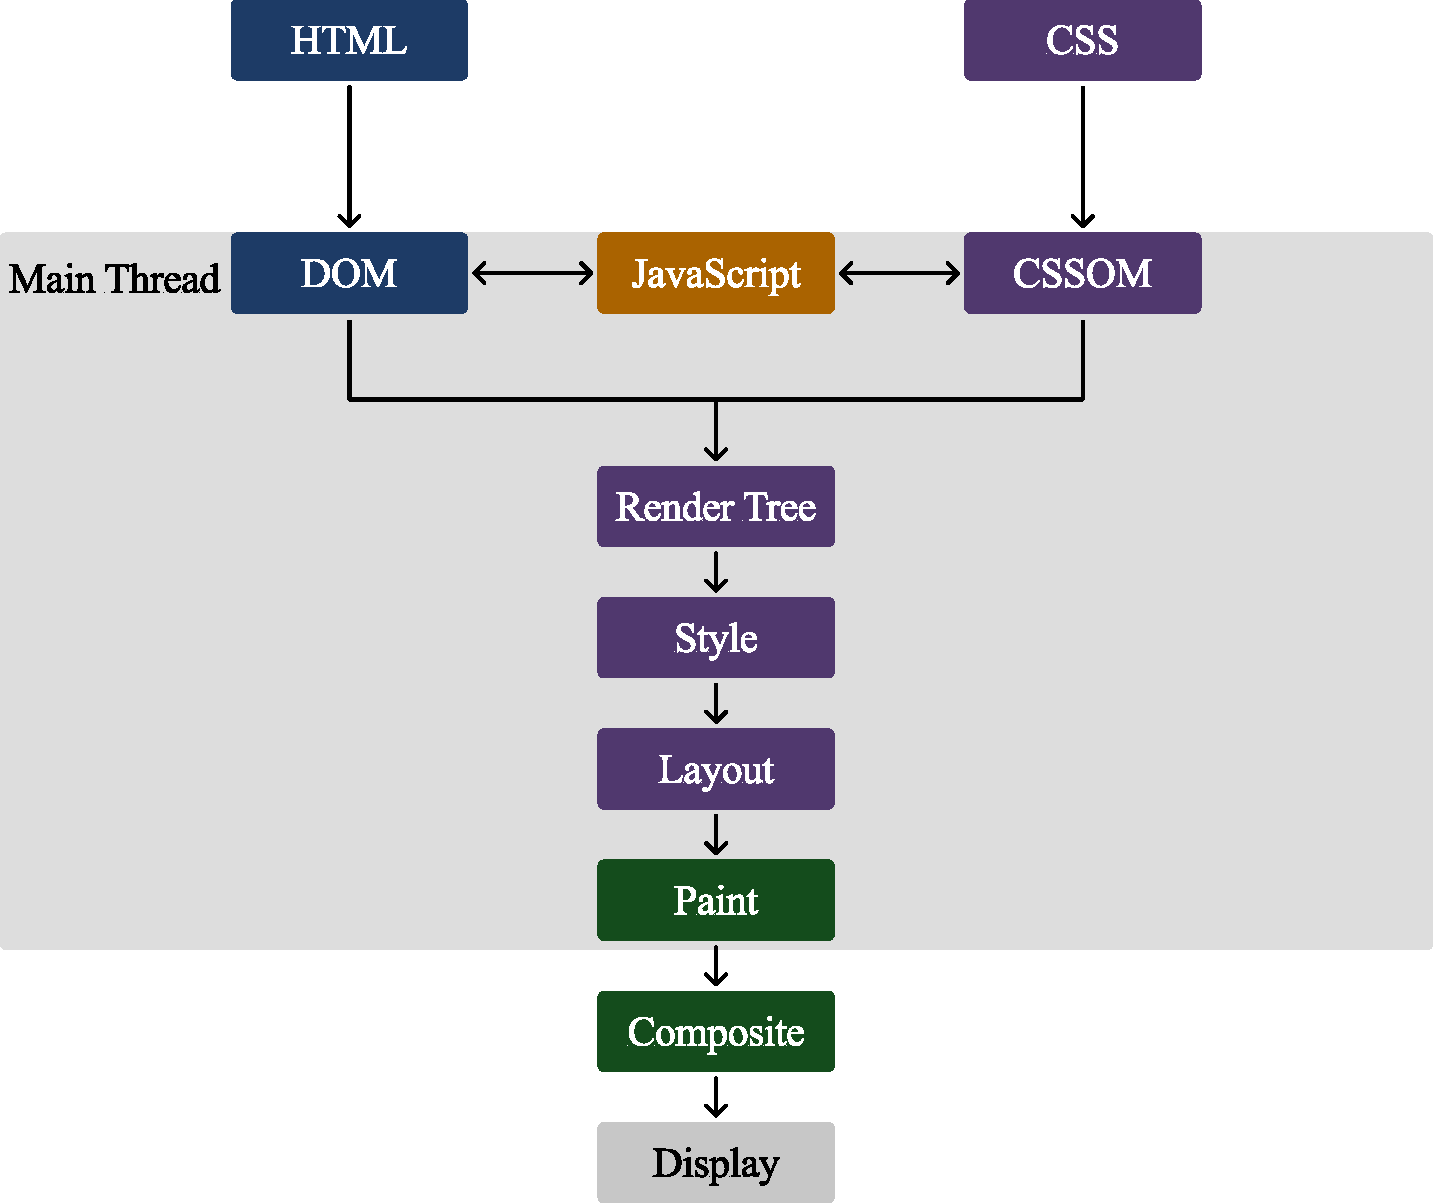
\includegraphics[width=0.8\textwidth,keepaspectratio]{bilder/rendering-pipeline.pdf}
	\caption[Phasenmodell des Critical Rendering Paths]{Phasenmodell des Critical Rendering Paths zur Verdeutlichung der Main-Thread-Auslastung (Eigene Darstellung in Anlehnung an \cite{web-dev-critical-path-2023}).}
	\label{fig:rendering-pipeline}
\end{figure}

\subsubsection{DOM als zentrale Repräsentation der UI}
\label{sss:dom}

Das DOM stellt die Inhalte hierarchisch in Form eines Baumes dar. Durch diese programmierbare Schnittstelle erhalten Skriptsprachen Zugriff auf die Objekte des Dokuments und können so Struktur und Inhalte flexibel verändern. Eltern-Kind-Beziehungen im DOM-Baum übersetzen die Verschachtelung des Quelltexts und bilden so die Grundlage für die Interaktivität moderner Webanwendungen \cite{mdn_dom_2026}. Jede dieser Änderungen am DOM kann dabei Rendering-Prozesse auslösen (vgl.\ \cref{sss:reflow-repaint-composite}).

\subsubsection{Sichtbarkeit im Render Tree und Layout-Abhängigkeiten}
\label{sss:visibility-render-tree-layout}

Bei der Modellbildung im Render Tree ist insbesondere zwischen \texttt{display: none} (nicht im Render Tree enthalten) und \texttt{visibility: hidden} (Elemente sind im Render Tree enthalten, belegen Layoutplatz, bleiben jedoch unsichtbar) zu unterscheiden \cite{web.dev_rclp_2014}. 
\Cref{fig:dom_cssom_render_tree} veranschaulicht diesen zentralen Unterschied zwischen logischer Struktur und visueller Repräsentation im Rahmen des Critical Rendering Paths. Während des Layout-Schritts wandelt der Browser die Knoten des Render Trees in konkrete Koordinaten um und bestimmt für jedes sichtbare Element innerhalb des Viewports, welche Ausmaße und Positionen es im Box-Modell einnimmt \cite{web.dev_rclp_2014}.
\begin{figure}[htb]
	\centering
	\narrowfig[0.7]{bilder/dom.pdf}
	\caption[Strukturelle Gegenüberstellung von DOM, CSSOM und Render Tree]{Strukturelle Gegenüberstellung von DOM, CSSOM und resultierendem Render Tree zur Veranschaulichung layoutrelevanter CSS-Eigenschaften. (Eigene Darstellung in Anlehnung an \cite{web.dev_rclp_2014}).}
	\label{fig:dom_cssom_render_tree}
\end{figure}

\subsubsection{Reflow, Repaint und Compositing: Performance-Kosten im Detail}
\label{sss:reflow-repaint-composite}

Je nach Art einer visuellen Änderung durchläuft der Browser die Rendering-Pipeline laut \cite{web.dev_rendering_2023} in drei unterschiedlichen Szenarien, die sich in ihrem Rechenaufwand stark unterscheiden. Eine Layout-Neuberechnung (Reflow) tritt auf, wenn sich geometrisch relevante Eigenschaften eines Elements ändern und der Browser dadurch die betroffenen und abhängigen Elemente im Layout erneut berechnen muss. Da Änderungen an einzelnen Elementen Auswirkungen auf die gesamte Hierarchie haben können, ist dieser Schritt besonders rechenintensiv. Handelt es sich um rein visuelle Anpassungen (z. B. Farbwechsel), führen diese lediglich zu einem Repaint, bei dem der Browser die betroffenen Pixelbereiche neu füllt, ohne die Geometrie erneut zu berechnen. Den effizientesten Weg stellt das Compositing dar, bei dem der Browser ausschließlich existierende Bildebenen (Layers) neu anordnet. Da dies oft auf einem eigenen Thread erfolgt, laufen insbesondere Animationen auf dieser Stufe besonders flüssig. Eine besondere Leistungsproblematik entsteht durch das sogenannte \textit{Layout Thrashing} \cite{web.dev_layoutthrashing_2025}. Dieses tritt auf, wenn JavaScript-Code Layout-Informationen abfragt (z. B. via \texttt{offsetWidth}), nachdem zuvor Stile verändert wurden \cite{web.dev_layoutthrashing_2025}. Da der Browser für die Abfrage einen aktuellen Wert liefern muss, erzwingt er eine sofortige, synchrone Neuberechnung (\textit{forced synchronous layout}), was zu einer ineffizienten Nutzung des Main Threads führt \cite{web.dev_layoutthrashing_2025}.

\subsection{Herausforderungen durch hochfrequente Updates (Main-Thread-Blocking)}
\label{ss:main-thread-blocking}

\subsubsection{Frame-Budget und Main-Thread-Überlastung}
\label{sss:frame-budget}

Damit eine Benutzeroberfläche flüssig wirkt, orientieren sich Browser nach \cite{web.dev_rendering_2023} an einer Bildwiederholrate von etwa 60 Bildern pro Sekunde. Daraus ergibt sich ein Zeitfenster von
\begin{equation}
	t_{\text{Frame}} = \frac{1000\,\mathrm{ms}}{60} \approx 16{,}7\,\mathrm{ms}
\end{equation}
pro Frame.
In der Praxis ist dieses Zeitfenster sogar noch knapper, da der Browser einen Teil dieser Zeit für interne Prozesse beansprucht. Letztlich verbleiben für die eigentliche Anwendungslogik oft nur etwa 10 ms. Innerhalb dieser kurzen Zeitspanne durchläuft der Browser die Rendering-Pipeline, die je nach Art der Änderung Prozesse wie die JavaScript-Ausführung, die Stil- und Layoutberechnung sowie das abschließende Painting und Compositing umfasst. Da diese Verarbeitungsschritte überwiegend sequenziell auf dem Main Thread ablaufen, führt jede Verzögerung innerhalb eines Einzelschritts zu einer Blockade des gesamten Renderprozesses \cite{mdn_mthread_2025}. Ergänzend definiert die Long Tasks API des World Wide Web Consortium (W3C) eine \qty{50}{ms}-Schwelle zur Identifikation blockierender Prozesse \cite{w3c_longtasks_2026}. Eine Aufgabe im Main Thread gilt als \textit{Long Task}, sobald ihre ununterbrochene Ausführungsdauer diesen Wert übersteigt.

\subsubsection{Auswirkungen auf Responsiveness und Benutzererfahrung}
\label{sss:user-expirience}

Ein häufiges Problem ist \textit{Input Delay}: Dabei verarbeitet der Browser Benutzereingaben wie Klicks oder Tastatureingaben nicht sofort, sondern erst nach Abschluss laufender Aufgaben, was zu einer spürbaren Verzögerung zwischen Eingabe und visueller Rückmeldung führt \cite{web.dev_inp_2025, w3c_longtasks_2026}. Als Maß für die Bewertung der Responsivität über die gesamte Besuchsdauer hinweg dient die Kennzahl INP (ausführliche Definition in \cref{ss:inp}). Ein weiteres Phänomen ist das sogenannte Jank \cite{web.dev_rendering_2023}. Dieses entsteht immer dann, wenn die Berechnung eines Frames länger dauert als das in \cref{sss:frame-budget} definierte Zeitfenster. Da der Browser in diesem Fall Frames überspringen muss, wirken Bewegungsabläufe wie Scrollen oder Animationen für den Nutzer stockend.

\subsubsection{Bedeutung für moderne UI-Frameworks (Synthese)}
\label{sss:ui-frameworks-synthesis}

Die in der Rendering-Pipeline entstehenden Kosten, insbesondere durch Layout- und Paint-Vorgänge (Reflows/Repaints), bilden die Grundlage für die Architektur moderner UI-Frameworks. Ziel dieser Frameworks ist es, die Anzahl direkter Eingriffe in das DOM zu minimieren. Anstatt jede Änderung sofort umzusetzen, bündelt das Framework Aktualisierungen. So ist sichergestellt, dass der Browser nur die tatsächlich veränderten Bereiche neu berechnen muss \cite{kumar-fluentreact-2024}. In der Praxis lassen sich dabei zwei unterschiedliche Strategien unterscheiden: Bibliotheken mit Virtual-DOM-Ansatz und compilerbasierte Frameworks. Diese grundlegenden Herangehensweisen werden in den folgenden Abschnitten detailliert analysiert.

\section{Architektur von React}
\label{s:react}

Dieser Abschnitt erläutert, wie React durch ein Virtual DOM (VDOM), Reconciliation und ergänzende Mechanismen diese Performance-Kosten adressiert.

\subsection{Virtual DOM und Reconciliation}
\label{ss:vdom}

Das VDOM ist eine Zwischenschicht im Speicher, die die Benutzeroberfläche mittels JavaScript-Objekten (React-Elementen) nachbildet. Wenn sich der Zustand (State) ändert, generiert React eine neue, virtuelle Darstellung des betroffenen React-Elementbaums. Durch das Bündeln mehrerer Änderungen (Batching) gibt React diese gesammelt an das reale DOM weiter, um die Anzahl teurer Layout-Neuberechnungen im Browser zu reduzieren \cite{kumar-fluentreact-2024}. Um die notwendigen Aktualisierungen zu identifizieren, nutzt React den Prozess der Reconciliation. Ein zentraler Bestandteil dieses Prozesses ist der Diffing-Algorithmus, ein rekursives Verfahren zum Vergleich der virtuellen Baumstrukturen. Während der Vergleich zweier beliebiger Baumstrukturen theoretisch eine Komplexität von $O(n^3)$ aufweist, reduziert React diesen Aufwand durch heuristische Annahmen (z. B. Elementtypen und Keys) in der Praxis auf annähernd $O(n)$ \cite{react_reconcillation_2024}. Da Zustandsänderungen standardmäßig Re-Renders entlang der nachgelagerten Teilbäume auslösen, steigt der Rechenaufwand dennoch direkt mit der Tiefe und Breite der betroffenen Komponentenstruktur \cite{kumar-fluentreact-2024}.


\subsection{Der React Compiler (ab React 19): Automatisierte Memoisierung vs. manuelles Opt-in}
\label{ss:react-compiler}

\subsubsection{Funktionsweise des React Compilers}
\label{sss:react-compiler}

Um unnötige Re-Renders zu vermeiden, mussten Entwickler bisher manuell mittels \texttt{React.memo} oder Hooks wie \texttt{useMemo} und \texttt{useCallback} memoisieren \cite{kumar-fluentreact-2024}. Diese Form der manuellen Memoisierung ist jedoch fehleranfällig und erhöht den kognitiven Aufwand während der Entwicklung \cite{react_introduction}. Der React Compiler verlagert diese Aufgaben in den Build-Prozess. Er untersucht den Code statisch mittels einer internen Zwischendarstellung (Intermediate Representation), analysiert den Datenfluss und fügt automatisch Optimierungen hinzu, die eine stabile Referenzgleichheit gewährleisten \cite{react_compiler_2025}. Im Gegensatz zu Svelte, welches Komponenten in DOM-nahen Code umwandelt, optimiert der React Compiler lediglich bestehende Komponenten durch intelligentes Caching, ohne das Laufzeitmodell grundlegend zu verändern \cite{kumar-fluentreact-2024}.


\subsubsection{Potenziale und Grenzen im Kontext der Skalierung}
\label{sss:potentials-and-limitations}

Die Automatisierung reduziert den Umfang an Boilerplate-Code und entlastet Entwickler von der Pflege von Abhängigkeitslisten (Dependency-Arrays) \cite{react_introduction}. Da der Compiler ausschließlich bestehende Komponenten memoisiert, bleiben die grundlegenden architekturbedingten Kosten von VDOM-Diffing und Reconciliation (\cref{ss:vdom}) sowie die damit verbundenen Heap-Allokationen jedoch bestehen \cite{kumar-fluentreact-2024, thedatascientist_vdom}.

\subsection{Fiber-Engine: Scheduling und Rendering}
\label{ss:fiber-engine}

Um synchron-blockierende Updates im Komponentenbaum zu verhindern, überarbeitete React die interne Verarbeitung grundlegend \cite{github-reactfiber-2016}.

\subsubsection{Aufbau der Fiber-Architektur}
\label{sss:fiber-engine-structure}

Fiber stellt eine interne Struktur zur Organisation und Planung von Arbeitsschritten (Scheduling) dar, wobei ein einzelner Fiber die kleinste unterbrechbare Arbeitseinheit repräsentiert \cite{github-reactfiber-2016}. Hierzu überführt Fiber den UI-Baum in eine mit expliziten Zeigern (Kind, Geschwister, Elternteil) verkettete Struktur, wodurch React laufende Prozesse bei Bedarf verwerfen, unterbrechen, den aktuellen Stand zwischenspeichern und die Ausführung ohne Kontextverlust später fortsetzen kann. Da Fiber den Call Stack lediglich nachbildet, bleibt die $O(n)$-Komplexität beim Diffing unverändert \cite{github-reactfiber-2016, react_reconcillation_2024}. Um diese Berechnungen ohne sofortige Auswirkung auf die Anzeige durchzuführen, nutzt die Architektur das Prinzip des \textit{Double Buffering}, bei dem ein im Hintergrund bearbeiteter Baum (\textit{work-in-progress}) erst nach Abschluss den sichtbaren Baum (\textit{current}) ersetzt, wie in \cref{fig:react_fiber_trees} veranschaulicht \cite{medium_fiber-2024}. Während Fiber-Knoten persistent sind und wiederverwendet werden, entstehen React-Elemente bei jedem Render-Vorgang neu \cite{dev_fiber-2018}. Die JavaScript-Engine V8 verwaltet diese kurzlebigen Objekte effizient im sogenannten \textit{jungen Speicherbereich} (Young Generation). Um die Auswirkungen auf den Main Thread bei der regelmäßigen Garbage Collection (GC) so gering wie möglich zu halten, lagert V8 diese Prozesse teilweise auf parallele Hilfs-Threads aus \cite{v8.dev_fiber-2019}. Wenn jedoch eine sehr hohe Anzahl an UI-Elementen gleichzeitig gerendert wird, summieren sich diese kleinen Rechen- und Speicheraufwände. Dadurch entsteht ein spürbarer Overhead, was die Skalierbarkeit im Vergleich zu Ansätzen ohne VDOM einschränken kann \cite{svelte_vdom-2018}.
\begin{figure}[H]
	\centering
	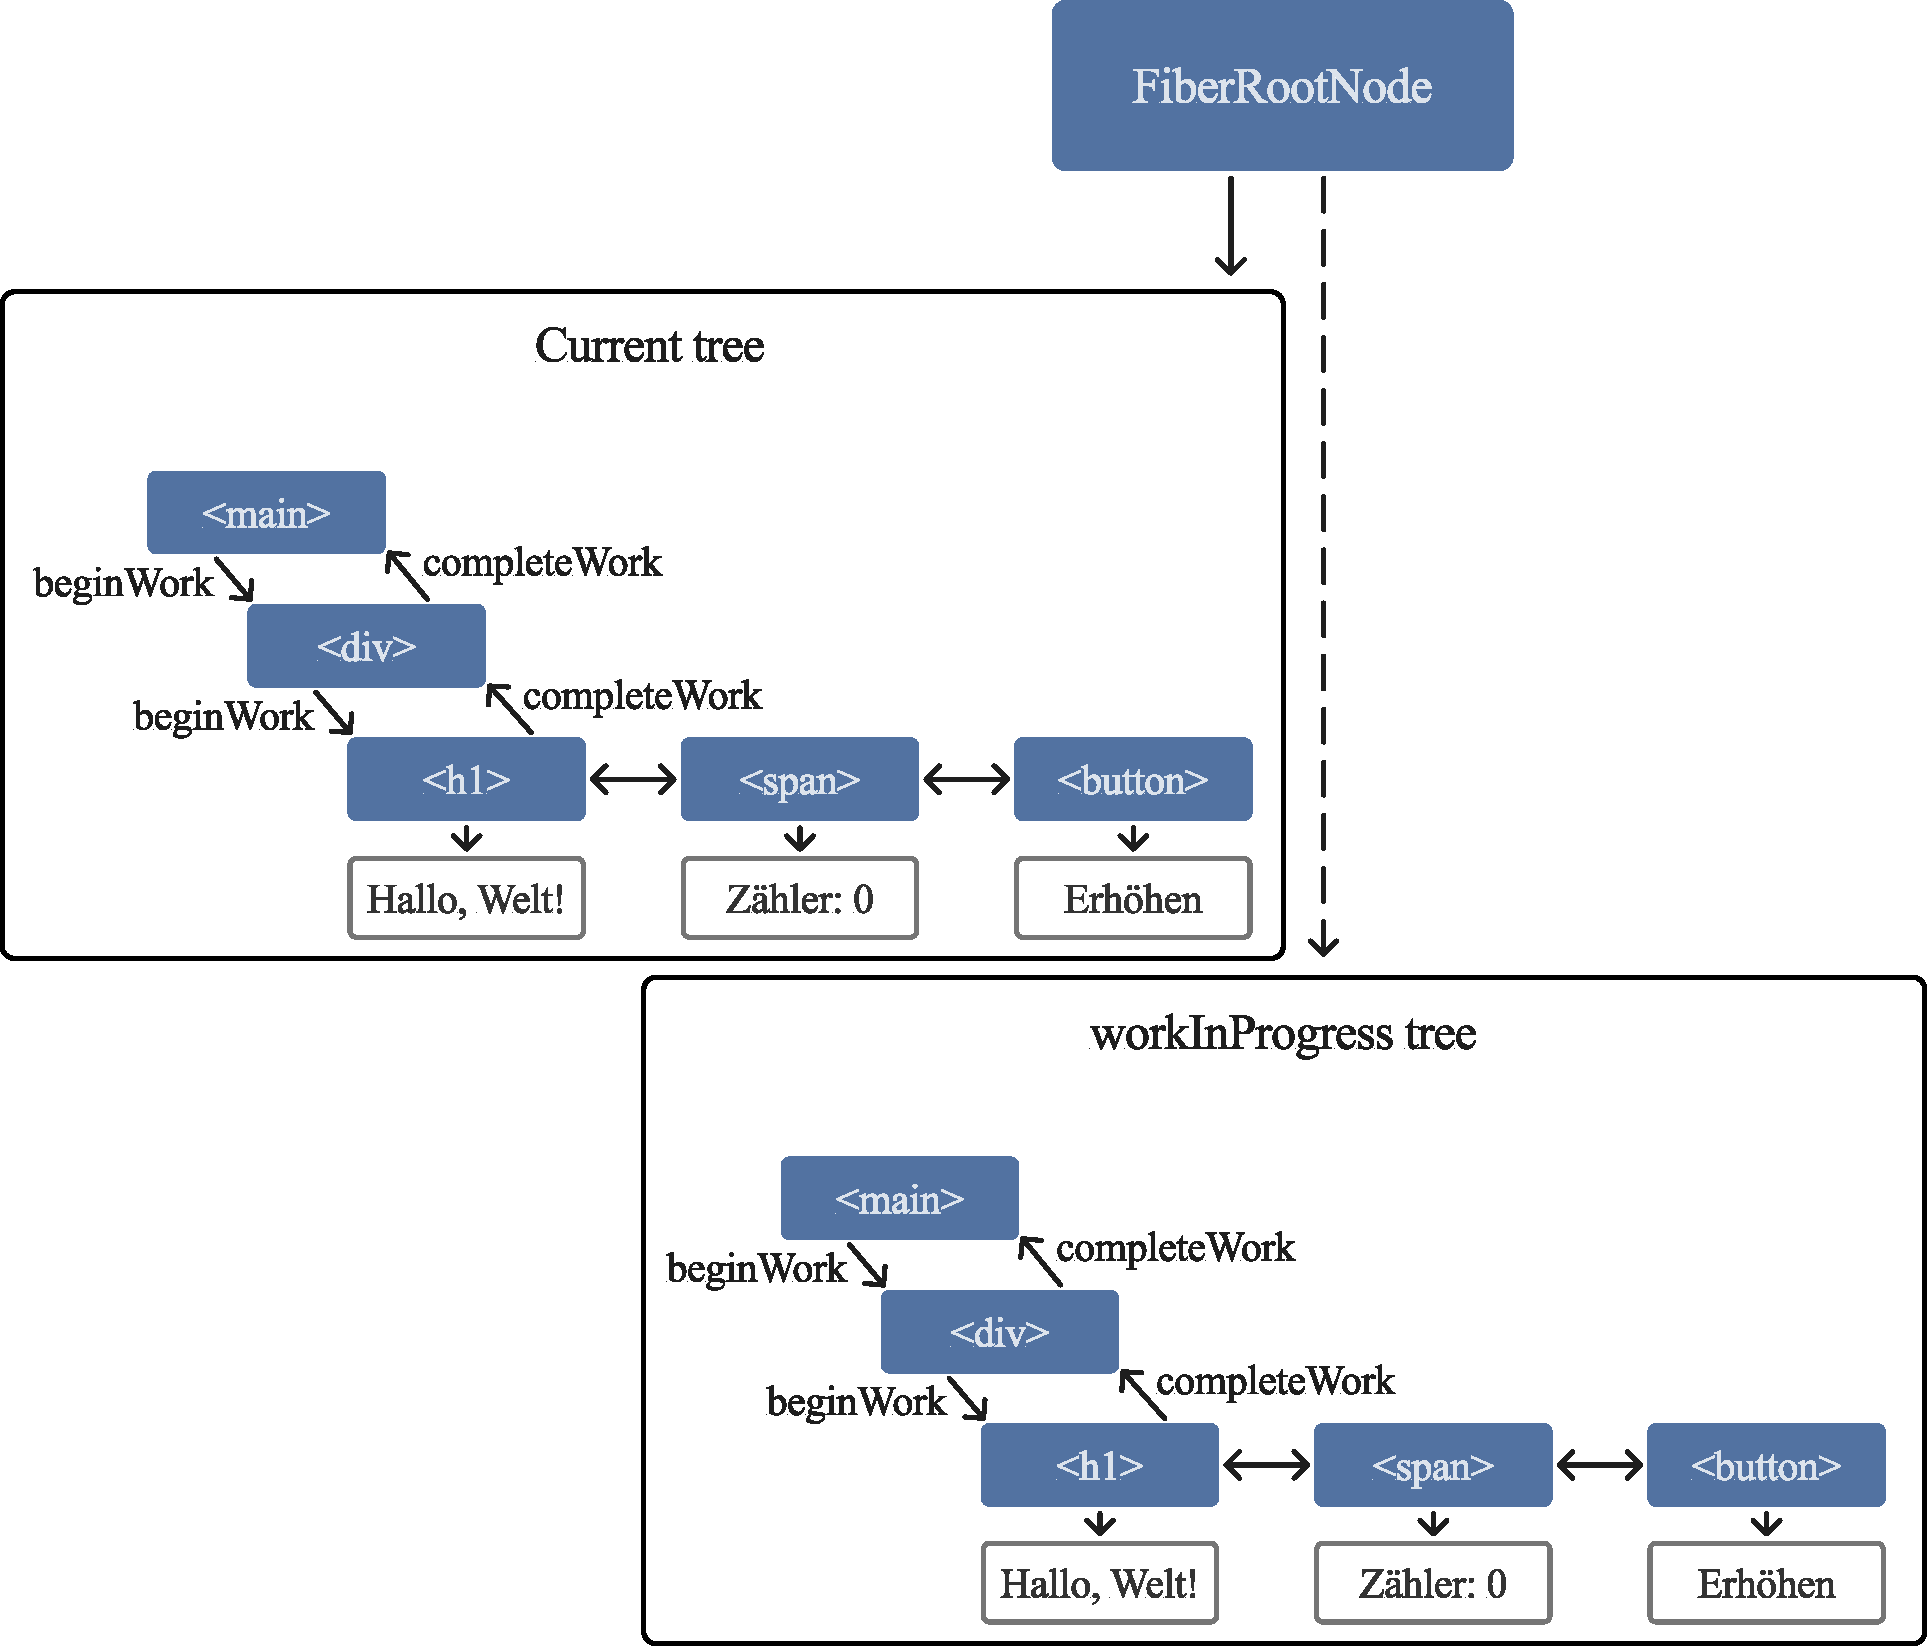
\includegraphics[width=0.8\textwidth,height=0.35\textheight,keepaspectratio]{bilder/fiber_double_buffering.pdf}
	\caption[Architekturmodell der React Fiber-Engine]{Architekturmodell der React Fiber-Engine: Double Buffering und Umschalten des FiberRootNode auf den Work-in-Progress Tree während der Commit-Phase. (Eigene Darstellung in Anlehnung an \cite{kumar-fluentreact-2024}).}
	\label{fig:react_fiber_trees}
\end{figure}

\subsubsection{Scheduling und Priorisierung von Updates}
\label{sss:scheduling-priotising-of-updates}

Um den Main Thread nicht zu blockieren, zerlegt das System anstehende Aufgaben per \textit{Time Slicing} in kleinere Arbeitsschritte. Über Render Lanes (Bitmasken) priorisiert das System Aufgaben nach Dringlichkeit: Nutzerinteraktionen (z. B. Klicks) erhalten stets Vorrang, Hintergrundprozesse laufen nachrangig \cite{kumar-fluentreact-2024}. Der Scheduler nutzt einen kooperativen Yielding-Ansatz: Nach der Bearbeitung einzelner Fiber-Knoten prüft der Scheduler, ob ein internes Zeitbudget (~5 ms) überschritten ist; ist dies der Fall, gibt er die Kontrolle an den Browser zurück \cite{dev_fiber-2025}. Übersteigt das Aufkommen an Updates die Kapazität des Schedulers, führt dieser Verarbeitungsstau zu verzögerten Render-Vorgängen und dazu, dass das Zeitfenster pro Frame trotz Priorisierung nicht mehr eingehalten werden kann \cite{sitepoint_fiber-2026}. Neben der Kompensation des Reconciliation-Overheads erfüllt das \textit{Time Slicing} eine weitere Funktion: Der kooperative Yielding-Ansatz begrenzt die maximale ununterbrochene Blockierungsdauer des Main Threads \cite{github-reactfiber-2016, react_concurrentrendering-2022}. Im Gegensatz dazu verfügt Svelte über kein integriertes \textit{Time Slicing} \cite{github-reactfiber-2016, medium-microtasks-2021}. Stattdessen fasst das Effect-Batching (\cref{sss:microtasks}) ausstehende Zustandsänderungen zusammen und arbeitet sie gebündelt im darauffolgenden Microtask ab \cite{svelte-effect}. Eine Verteilung noch ausstehender Arbeit auf nachfolgende Frames ist in dieser Architektur nicht vorgesehen \cite{medium-microtasks-2021, github-reactfiber-2016}.


\subsubsection{Concurrent Rendering}
\label{sss:concurrent-rendering}

Aufbauend auf der Fiber-Struktur und der Priorisierung ermöglicht Concurrent Rendering die Vorbereitung neuer UI-Zustände im Hintergrund, ohne die sichtbare Oberfläche direkt zu verändern \cite{react_concurrentrendering-2022}. Für eine hohe Reaktionsfähigkeit gliedert sich der Ablauf in zwei Phasen \cite{medium_fiber-2018}:
\begin{enumerate}
	\item \textbf{Render-Phase (asynchron):} Das System identifiziert mittels Diffing die erforderlichen Änderungen. Dieser Prozess ist unterbrechbar.
	\item \textbf{Commit-Phase (synchron):} React nimmt die Änderungen am realen DOM vor. Dieser Schritt ist stets synchron und nicht unterbrechbar \cite{medium_fiber-2018}.
\end{enumerate}
Die Dauer der Commit-Phase hängt direkt von der Anzahl der zu aktualisierenden DOM-Elemente ab \cite{kumar-fluentreact-2024}. Bei hoher UI-Dichte kann diese Phase das Frame-Budget ununterbrechbar belegen, was zu Jank führt und die Interaktionslatenz (INP) unmittelbar verlängert \cite{web.dev_fiber_2025}.

\section{Architektur von Svelte}
\label{s:svelte}

Während der in \cref{s:react} untersuchte Ansatz von React stark auf eine komplexe Laufzeitumgebung und den Vergleich eines VDOM setzt, wählt Svelte einen anderen Ansatz. Statt Änderungen erst im Browser zur Laufzeit zu berechnen, verlagert Svelte diese Arbeit in den Build-Prozess \cite{github-svelte_arch-2017}.

\subsection{Compilerbasierter Ansatz}
\label{ss:svelte-compiler}

Beim Build-Prozess überführt der Compiler den deklarativen Code in einen abstrakten Syntaxbaum (AST) und generiert daraus spezifische Code-Fragmente für das Erstellen, Aktualisieren und Entfernen einzelner DOM-Knoten \cite{github-svelte_arch-2017, svelte_vdom-2018}. Welche dieser Fragmente bei einer Datenänderungen ausgeführt werden, bestimmt in Svelte 5 die Signal-Architektur zur Laufzeit (vgl.\ \cref{ss:svelte-reactivity}), sodass das System ausschließlich die unmittelbar betroffenen Operationen ausführt. Durch den Verzicht auf ein VDOM und die damit verbundenen Reconciliation-Prozesse reduziert sich die Rechenlast auf dem Main Thread sowie der Speicherbedarf erheblich \cite{svelte_vdom-2018, ollila-rendering_performance-2022}. Dies führt zu weniger Objektzuweisungen im Heap und entlastet die Garbage Collection, wodurch pro Frame mehr Zeit für eine flüssige Darstellung zur Verfügung steht \cite{svelte-reactivity-2019}.

\subsection{Reaktivität und Update-Mechanismen}
\label{ss:svelte-reactivity}

Im Gegensatz zum klassischen Svelte-Compiler, der Abhängigkeiten ausschließlich statisch zur Kompilierzeit ermittelt hat, setzt Svelte 5 auf das Modell der Signals \cite{svelte_runes_2023}. Entwickler nutzen hierzu spezifische Compiler-Anweisungen, sogenannte Runes (z. B. \texttt{\$state} und \texttt{\$derived}). Während Runes die syntaktische Schnittstelle bilden, identifizieren Signals zur Laufzeit automatisch die Abhängigkeiten zwischen den Werten \cite{svelte_migration}.

\subsubsection{Mechanismus der feingranularen Reaktivität}
\label{sss:finegraned-reactivity}

Die Signal-Architektur ermöglicht eine feingranulare Reaktivität \cite{svelte_runes_2023, balasubramanian-signal-2025}, bei der die gesamte Verarbeitung, von der Erkennung einer Zustandsänderung über die Auswertung der betroffenen Abhängigkeiten bis zur gezielten DOM-Aktualisierung, auf die jeweils betroffenen Knoten begrenzt bleibt \cite{svelte_runes_2023, balasubramanian-signal-2025}. Zustandsänderungen lassen sich so auch bei Arrays aus primitiven Datentypen genau nachverfolgen, ohne die ursprüngliche Datenstruktur anzupassen \cite{svelte_fine-grained_reactivity-2023}. Im Vergleich zur Reconciliation in React, die oft mehrere Abgleichschritte über Teilbäume erfordert, reduziert dieser Ansatz den Aufwand pro Interaktion meist auf eine einzige gezielte Operation \cite{putra-performance-2025}.

\subsubsection{Speichermodell und Overhead von Runes}
\label{sss:runes-overhead}

Intern bildet Svelte Signals als einfache JavaScript-Objekte (POJOs) ab, die sowohl bei der Erstellung als auch beim Zugriff deutlich ressourcensparender sind als komplexe Klasseninstanzen \cite{github-svelte_bench_13277-2024}. Im Unterschied zu den baumartigen Fiber-Strukturen von React (\cref{sss:fiber-engine-structure}) schafft dieser compilerbasierte Ansatz die strukturellen Voraussetzungen für eine effizientere Skalierung, insbesondere bei großen Mengen an UI-Elementen \cite{putra-performance-2025}. Der Overhead pro Signal ist zwar minimal, doch bei jedem Update muss das System jede reaktive Abhängigkeit einzeln auswerten (\cref{sss:finegraned-reactivity}). Bei gleichzeitiger Aktualisierung aller $n$ Elemente wächst der Gesamtaufwand ebenfalls mit $O(n)$ — dieselbe Komplexitätsklasse wie die Reconciliation in React (\cref{ss:vdom}), allerdings mit einem geringeren Aufwand pro Element. Ab welchem $n$ dieser Unterschied praktisch vernachlässigbar wird, lässt sich theoretisch nicht bestimmen.

\subsubsection{Vermeidung von Render-Flaschenhälsen}
\label{sss:rendering-bottleneck}

Die feingranulare Signal-Architektur reduziert die CPU-Belastung deutlich, da die Implementierung gezielt darauf ausgelegt ist, ineffiziente Ausführungen in der JavaScript-Engine (V8) zu vermeiden und besonders häufig genutzte Codebereiche (\textit{Hot Paths}) zu optimieren \cite{github-svelte_bench_13277-2024}. In Kombination mit sehr schnellen Ausführungszeiten und nur minimalen Eingriffen ins DOM sinkt dadurch die Wahrscheinlichkeit für Long Tasks (\cref{sss:frame-budget}). Daraus lässt sich ableiten, dass Svelte selbst unter hoher Last kein aufwendiges Laufzeit-Scheduling wie etwa das Time Slicing in React benötigt, da die einzelnen Verarbeitungsschritte von vornherein klein und effizient gehalten sind.


\subsection{Effizienz der imperativen DOM-Updates}
\label{ss:svelte-efficiency}

\subsubsection{Ausführung imperativer DOM-Befehle}
\label{sss:running-dom-commands}

Zur Erstellung von DOM-Strukturen nutzt der Compiler Verfahren wie das Klonen von \texttt{<template>}-Elementen oder den schrittweisen programmatischen Aufbau \cite{svelte-compiler}. Die Darstellung von Template-Ausdrücken und deren Logik basiert intern auf Effekten. Diese sorgen automatisiert dafür, dass Datenänderungen unmittelbar zu einer Anpassung des DOM führen. Für Spezialfälle, in denen bestimmte Operationen noch vor der eigentlichen DOM-Aktualisierung erfolgen müssen, stellt Svelte zusätzlich \texttt{effect.pre} bereit \cite{svelte-effect}.


\subsubsection{Effect-Batching und Microtasks}
\label{sss:microtasks}

Ändert sich der Zustand in einer Svelte-Anwendung, passt Svelte das DOM nicht sofort nach jeder einzelnen Änderung an \cite{medium-microtasks-2021}. Stattdessen bündelt Svelte Zustandsänderungen per Microtask: Das Framework fasst mehrere gleichzeitige Änderungen zusammen, bevor DOM-Anpassungen und Effects folgen \cite{svelte-effect}. Dadurch lässt sich das in \cref{sss:reflow-repaint-composite} beschriebene Layout Thrashing wirksam vermeiden. 


\subsubsection{Theoretische Grenzen (JS-zu-DOM-Flaschenhals)}
\label{sss:theoretical-limitations}

Trotz dieser Optimierungen bleibt Svelte an die grundlegenden Grenzen der Browser-Architektur gebunden. Zwar sind die JavaScript-Engine und die Rendering-Engine eigenständige Komponenten, sie arbeiten jedoch über klar definierte Schnittstellen wie das DOM und die Web-IDL-Bindings eng zusammen \cite{mdn-javascript_engine}. Jeder Zugriff auf diese Verbindung zwischen JavaScript und der Rendering-Schicht bringt dabei einen systembedingten Overhead mit sich \cite{chromium-blink_faq}. Bei einer extremen kombinierten Last aus UI-Dichte und Update-Frequenz können daher auch unter Svelte blockierende Long Tasks und Interaktionslatenzen auftreten, da sich die Kosten für wiederholte DOM-Zugriffe summieren (\cref{sss:frame-budget}).

\section{Vergleichbare Metriken und Performancebegriffe}
\label{s:metrics}

\subsection{Interaktionslatenz und Antwortverhalten (INP)}
\label{ss:inp}

\subsubsection{Definition und Phasen der Metrik}
Die Metrik Interaction to Next Paint (INP) misst, wie schnell eine Webseite auf Nutzerinteraktionen über die gesamte Nutzungsdauer hinweg reagiert \cite{web.dev_inp_2025}. Die technische Zusammensetzung der Metrik sowie die zeitliche Abfolge der einzelnen Phasen sind in \cref{fig:inp-phases} dargestellt. Aus technischer Sicht lässt sich dieser Messwert in drei Phasen unterteilen \cite{web.dev_inp_2025}:
\begin{itemize}
	\item \textbf{Input Delay (Eingabeverzögerung):} Zeitspanne vom Beginn der Nutzerinteraktion bis zur Verarbeitung des ersten Event-Handlers, verursacht durch Main-Thread-Blockaden (vgl. \cref{ss:main-thread-blocking}).
	\item \textbf{Processing Time (Verarbeitungsdauer):} Hierbei handelt es sich um die Zeit zur vollständigen Ausführung aller Callbacks der Event-Handler und der damit verbundenen Framework-Logik.
	\item \textbf{Presentation Delay (Darstellungsverzögerung):} Diese Phase misst die Zeit nach Abschluss der Skriptausführung bis zu dem Punkt, in dem der Browser die Änderungen sichtbar auf dem Bildschirm darstellt.
\end{itemize}
Google definiert auf Basis dieser Metrik drei Leistungskategorien: INP-Werte bis einschließlich $200\,\text{ms}$ gelten als \textit{Good}; Werte zwischen $200\,\text{ms}$ und $500\,\text{ms}$ als \textit{Needs Improvement}; Werte oberhalb von $500\,\text{ms}$ als \textit{Poor} \cite{web.dev_inp_2025}.
\begin{figure}[H]
	\centering
	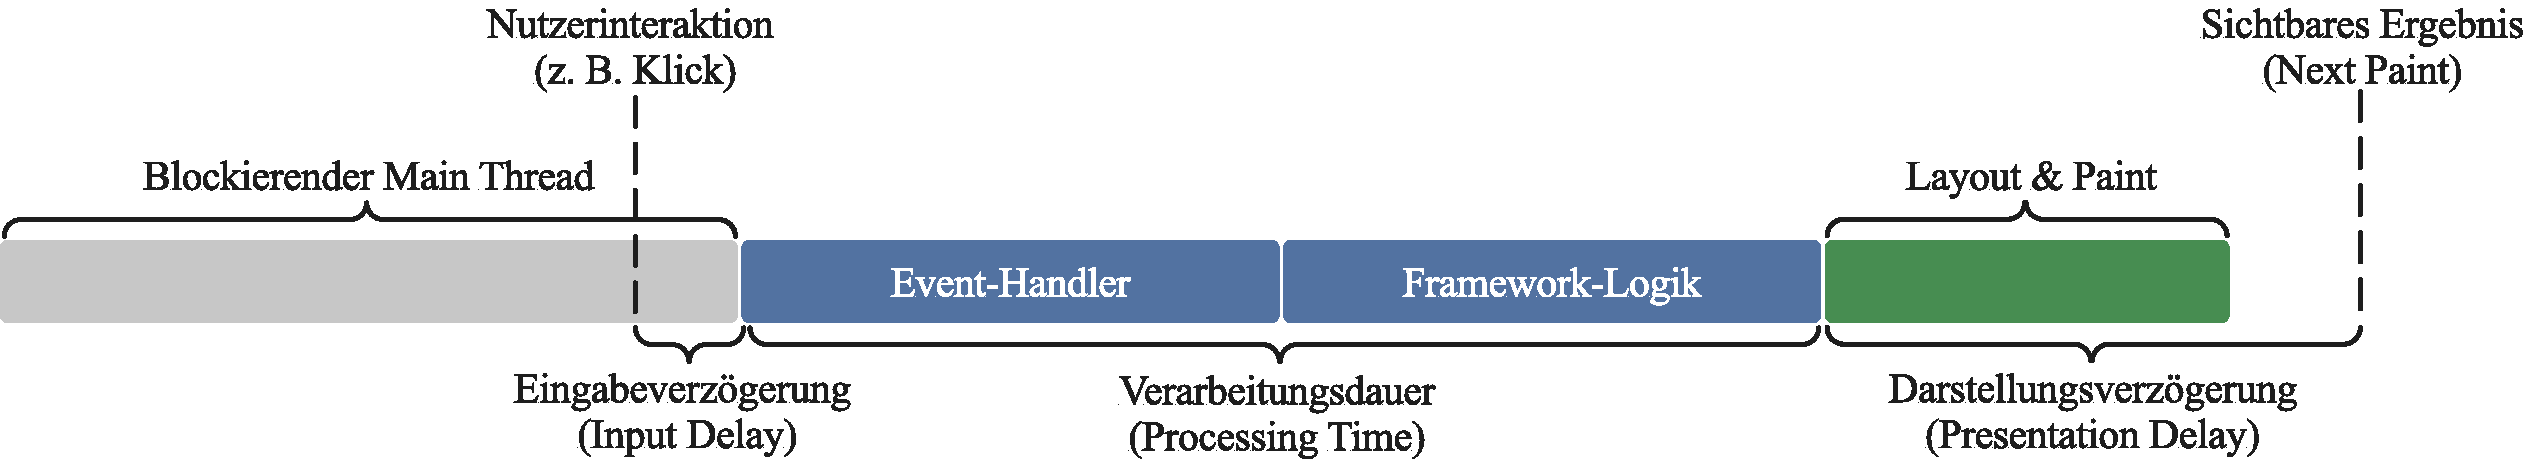
\includegraphics{bilder/inp_phasenmodell.pdf}
	\caption[Zeitliches Phasenmodell der INP-Metrik]{Zeitliches Phasenmodell der Metrik Interaction to Next Paint (INP) vom Auslösen des Events bis zum Rendering. (Eigene Darstellung in Anlehnung an \cite{web.dev_inp_2025}).}
	\label{fig:inp-phases}
\end{figure}

\subsubsection{Messung aller Interaktionen und Abgrenzung zu FID}
Im Gegensatz zum \textit{First Input Delay} (FID), welcher nur die erste Interaktion erfasst, bewertet INP die Stabilität der Performance während der gesamten Sitzung. Der finale INP-Wert entspricht in der Regel der Interaktion mit der höchsten Gesamtverzögerung. Damit einzelne Ausreißer das Ergebnis nicht verzerren, ignoriert die Metrik bei jeweils 50 Interaktionen den höchsten Wert. Auf diese Weise entsteht ein realistischeres Bild der tatsächlichen, stabilen Performance \cite{web.dev_inp_2025}.

\subsubsection{Relevanz für die Messung der UI-Skalierung}
INP dient als zentrale Metrik, um den in \cref{sss:tipping-point} beschriebenen Tipping Point empirisch zu identifizieren. Sie macht messbar, ab welcher kombinierten Last aus UI-Dichte und Update-Frequenz die \textit{Processing Time} oder das \textit{Presentation Delay} das verfügbare Frame-Budget überschreitet und zu spürbaren Verzögerungen führt.


\subsection{Analyse der Speichereffizienz (Heap-Snapshots)}
\label{ss:memory-efficiency}

\subsubsection{Funktionsweise von Heap-Snapshots}
Ein Heap-Snapshot stellt eine detaillierte Momentaufnahme des Objektgraphen innerhalb des Speichers der JavaScript-Laufzeitumgebung dar \cite{chrome-memory-terminology-2024}. Er dient dazu, die Speicherverteilung zu untersuchen, mögliche Speicherlecks zu erkennen oder Objekte zu identifizieren, die übermäßig viele Ressourcen im System beanspruchen \cite{chrome-heap-snapshots-2024}.

\subsubsection{Shallow Size vs. Retained Size}
Zur genauen Messung des Speicherverbrauchs sind zwei zentrale Metriken zu unterscheiden: Die \textit{Shallow Size} umfasst den Speicherplatz, den ein Objekt für sich selbst beansprucht, ohne dabei den Speicher der referenzierten Objekte einzubeziehen.
Die \textit{Retained Size} hingegen beschreibt, wie viel Speicher freigegeben werden kann, wenn ein bestimmtes Objekt aus dem Speicher entfernt wird. Sie umfasst dabei nicht nur das Objekt selbst, sondern auch alle abhängigen Elemente, die ausschließlich über dieses Objekt referenziert wurden und nach dessen Entfernung keine Verbindung mehr zu den Garbage-Collector-Wurzeln haben \cite{chrome-memory-terminology-2024}.

\subsubsection{Analyse des Objekt-Graphen: Distance und Dominators}

Die \textit{Distance} gibt die Anzahl der Schritte von der Wurzel des Garbage Collectors (GC Root) zum Objekt an. Weisen Objekte gleichen Typs ungewöhnlich große Distanzen auf, deutet das oft auf komplexe und speicherintensive Referenzketten hin \cite{chrome-memory-terminology-2024}. Strukturell basiert die Retained Size im Wesentlichen auf dem Konzept der \textit{Dominators} (Dominatoren). Dabei gilt ein Objekt $d$ als Dominator eines anderen Objekts $n$, wenn jeder mögliche Pfad vom Root-Knoten zu $n$ zwangsläufig über $d$ führt \cite{bynens-lorenz-memory-profiling}. Innerhalb des Speicher-Graphen lassen sich Dominator-Beziehungen als Baumstruktur darstellen \cite{chrome-memory-terminology-2024}. Diese Struktur ist besonders wichtig für die Retained Size, da beim Entfernen eines Objekts auch alle davon abhängigen Objekte im zugehörigen Zweig für die Garbage Collection freigegeben werden. Diese baumartige Hierarchie sowie das Zusammenspiel der Metriken Distance, Shallow Size und Retained Size werden in \cref{fig:heap_dominator_tree} zusammenfassend visualisiert. Für den empirischen Framework-Vergleich ist die Retained Size die geeignetste Kennzahl, da sie den internen Framework-Overhead vom Anwendungszustand trennt. Die methodische Umsetzung dieser Messung erläutert \cref{ss:memory-measurement}.
\begin{figure}[H]
	\centering
	\narrowfig[0.7]{bilder/heap_dominator_tree.pdf}
	\caption[Modell eines Speicher-Graphen zur Darstellung der Retained Size]{Modell eines Speicher-Graphen zur Veranschaulichung der Dominator-Beziehungen sowie der Differenzierung zwischen Shallow und Retained Size. (Eigene Darstellung in Anlehnung an \cite{chrome-memory-terminology-2024}).}
	\label{fig:heap_dominator_tree}
\end{figure}

\subsection{Scripting- vs. Rendering-Zeit im Browser-Profil}
\label{ss:profiling-categories}

\subsubsection{Kategorien im Performance-Trace}
Werkzeuge wie das Chrome DevTools Performance-Panel visualisieren die Main-Thread-Auslastung in Kategorien \cite{chrome-performance-reference-2024}:

\begin{itemize}
	\item \textbf{Scripting (Gelb):} Diese Kategorie beschreibt die gesamte Zeit, die die JavaScript-Engine für das Parsen, Kompilieren und Ausführen von JavaScript-Code benötigt \cite{chrome-lighthouse-js-execution-2019, chrome-performance-reference-2024}.
	
	\item \textbf{Rendering (Lila):} Die \textit{Rendering-Zeit} umfasst alle Phasen, in denen der Browser nach Zustandsänderungen die Stile der Elemente neu berechnet (\textit{Recalculate Style}) und anschließend die Geometrie des Dokumentenbaums bestimmt (\textit{Layout}) \cite{chrome-performance-reference-2024}.
	
	\item \textbf{Painting:} Diese Phase beschreibt den Prozess, bei dem der Browser die grafischen Zeichenbefehle in Pixel umwandelt, bevor der Browser diese im nächsten Schritt final zur Bildschirmausgabe zusammensetzt \cite{chromium-frameviewer-howto}. 
\end{itemize}

\subsubsection{Bedeutung für die Tipping-Point-Analyse}

Die getrennte Analyse dieser Kategorien hilft dabei zu erkennen, wo Leistungsengpässe entstehen. Während die \textit{Scripting-Zeit} den internen Aufwand der Framework-Logik (z. B. Reconciliation oder Signal-Auswertung) widerspiegelt, zeigt die Rendering-Zeit die Last der Browser-Engine beim Umsetzen der DOM-Änderungen \cite{chrome-performance-reference-2024, chromium-frameviewer-howto}. Dies ist essenziell für die Untersuchung der theoretischen Skalierungsgrenzen (\cref{sss:theoretical-limitations}).


\section{Theoretische Vergleichsmodelle und Hypothesen}
\label{s:theoretical-models-and-hypotheses}

Dieses Kapitel überführt die architektonischen Merkmale aus \cref{s:react} und \cref{s:svelte} in ein vergleichendes Modell. Ziel ist es, die Auswirkungen von UI-Dichte ($n$) und Update-Frequenz ($f$) auf die Systemleistung theoretisch herzuleiten.

\subsection{Synthese der Abstraktionskosten}
\label{ss:abstraction-costs}

Der Vergleich zwischen dem VDOM-basierten Ansatz und der direkten DOM-Manipulation zeigt grundlegende Unterschiede in der Ressourcenallokation. Während der in \cref{ss:vdom} beschriebene Diffing-Prozess von React bei Zustandsänderungen einen algorithmischen CPU-Overhead zur Laufzeit verursacht, entfällt dieser Reconciliation-Overhead bei der Compiler-Architektur von Svelte (\cref{ss:svelte-compiler}) fast vollständig. Dies betrifft auch den Speicherbedarf: Durch den VDOM-Ansatz werden fortlaufend virtuelle Knoten erzeugt, wodurch die Belastung der Garbage Collection linear mit der Anzahl der Elemente $n$ ansteigt \cite{bai-millionjs-2023, github-reactfiber-2016}. Svelte umgeht diese Zwischenstrukturen und entlastet so die JavaScript-Laufzeitumgebung (\cref{ss:svelte-compiler}). Unabhängig davon sind beide Architekturen jedoch auf die native DOM-Schnittstelle angewiesen, was bei hoher Skalierung zu einem unvermeidbaren Flaschenhals im Main Thread führt (\cref{sss:theoretical-limitations}).

\subsection{Komplexität und Skalierung (n vs. f)}
\label{ss:update-complexity}

\subsubsection{Umfang der Neuberechnungen bei Zustandsänderungen} 

In der React-Architektur skaliert der Berechnungsaufwand bei Zustandsänderungen unabhängig von tatsächlichen DOM-Veränderungen direkt proportional zur Anzahl der Knoten im betroffenen Teilbaum (\cref{ss:vdom}). Im Gegensatz dazu entkoppelt das feingranulare Reaktivitätsmodell von Svelte (\cref{ss:svelte-reactivity}) den Aufwand von der Baumgröße. Da keine Diffing-Schritte über nicht betroffene Komponenten nötig sind, bestimmt sich die Ausführungszeit primär durch die Anzahl der tatsächlich veränderten Abhängigkeiten (\cref{sss:finegraned-reactivity}).

\subsubsection{Der Multiplikator-Effekt und der Tipping Point}
\label{sss:tipping-point}

Die Kombination aus hoher Frequenz $f$ und hoher Dichte $n$ führt zu einer gegenseitigen Verstärkung der Last. Da React bei jeder Änderung den entsprechenden Teilbaum erneut überprüft (\cref{ss:vdom}), kann die CPU-Auslastung bei hoher UI-Dichte und gleichzeitig hoher Aktualisierungsrate das Frame-Budget von 16,7 ms (\cref{sss:frame-budget}) vergleichsweise schnell ausschöpfen. Svelte begrenzt diesen Effekt durch direkte Operationen am relevanten Knoten (\cref{sss:finegraned-reactivity}). Aus den architektonischen Skalierungsunterschieden lässt sich ein theoretischer Tipping Point ableiten. Dieser bezeichnet den Übergang, an dem die aufsummierte Last den Main Thread durch Long Tasks blockiert (\cref{sss:frame-budget}). Bedingt durch baumgrößenabhängige Re-Render-Zyklen und die synchrone, nicht unterbrechbare Commit-Phase (\cref{sss:concurrent-rendering}) ist davon auszugehen, dass React diesen Punkt früher erreicht als Svelte. Bei vollständiger Aktualisierung aller $n$ Elemente pro Tick wächst auch der Aufwand der feingranularen Reaktivität linear mit $n$ (\cref{sss:runes-overhead}). Ab einem bestimmten Sättigungspunkt kann daher auch Svelte den Main Thread durch Long Tasks blockieren (\cref{sss:theoretical-limitations}). Da Sveltes Effect-Batching die gesamte Verarbeitung synchron innerhalb desselben Microtask-Zyklus abschließt (\cref{sss:microtasks}), während Reacts Time Slicing Arbeitsschritte über mehrere Frames verteilen kann (\cref{sss:scheduling-priotising-of-updates}), ist eine Umkehr der Tipping-Point-Rangfolge bei extremer kombinierter Last theoretisch nicht auszuschließen.


\subsection{Erwartetes Skalierungsverhalten}
\label{ss:expected-scaling}

Aus den in \cref{ss:update-complexity} beschriebenen Skalierungsunterschieden lässt sich erwarten, dass die Scripting-Zeit beider Frameworks unterschiedlich stark mit $n$ wächst. Die Reconciliation durchläuft dabei stets den gesamten betroffenen Teilbaum mit $O(n)$, unabhängig davon, wie viele Knoten sich tatsächlich verändert haben (\cref{ss:vdom}). Hinzu kommt der in \cref{sss:fiber-engine-structure} beschriebene GC-Overhead durch kurzlebige React-Elemente, der konzeptionell linear mit $n$ wächst (\cref{ss:abstraction-costs}). Svelte hingegen begrenzt den Scripting-Aufwand durch die feingranulare Reaktivität (\cref{sss:finegraned-reactivity}) auf die Auswertung der tatsächlich veränderten Abhängigkeiten. Da keine Diffing-Schritte über unveränderte Komponenten anfallen (\cref{ss:update-complexity}), ist davon auszugehen, dass der Aufwand nicht mit der Gesamtgröße des Komponentenbaums wächst, sondern mit der Anzahl der Änderungen. Auch wenn beide Architekturen bei vollständiger Aktualisierung mit $O(n)$ skalieren, ist der Aufwand pro Element bei Svelte theoretisch geringer, da der Abgleich des Komponentenbaums und die damit verbundenen Heap-Allokationen entfallen (\cref{sss:runes-overhead}). Aus diesem Unterschied ergibt sich die Annahme, dass der Scripting-Aufwand pro Tick in React stärker mit $n$ wächst als in Svelte. Bei vollständiger Aktualisierung aller $n$ Elemente wertet Svelte ebenfalls $n$ Abhängigkeiten aus; der verbleibende Vorteil besteht ausschließlich im geringeren Aufwand pro Element (\cref{sss:runes-overhead}). Über die Skalierung der Scripting-Zeit hinaus lassen sich auch Auswirkungen auf die Interaktionslatenz (INP) ableiten. Für \textbf{React} kann Concurrent Rendering (\cref{sss:concurrent-rendering}) das Input Delay stabilisieren, indem das System rechenintensive Render-Vorgänge unterbricht und Nutzerinteraktionen priorisiert (\cref{sss:scheduling-priotising-of-updates}). Ab einem bestimmten Sättigungspunkt belegt die nicht unterbrechbare, synchrone Commit-Phase den Main Thread jedoch so lange (\cref{sss:concurrent-rendering}), dass das System nachfolgende Eingaben verzögert verarbeitet. Dies kann sowohl das \textit{Input Delay} als auch das Presentation Delay erhöhen (\cref{ss:inp}) und sich negativ auf die Interaktionslatenz (INP) auswirken. Für \textbf{Svelte} ist aufgrund des geringeren Aufwands pro Tick eine Überlastung des Main Threads erst bei höherer Last zu erwarten. Allerdings schließt Sveltes Effect-Batching (\cref{sss:microtasks}) die gesamte Aktualisierung synchron ab, ohne Arbeit auf Folge-Frames zu verteilen (\cref{sss:scheduling-priotising-of-updates}). Im Gegensatz dazu ermöglicht Reacts kooperatives Yielding (\cref{sss:scheduling-priotising-of-updates}) eine Unterbrechung zugunsten von Nutzerinteraktionen. Daraus lässt sich ableiten, dass bei Last unterhalb des Frame-Budgets (\cref{sss:frame-budget}) Reacts Scheduling die INP stabilisieren kann, auch wenn die absoluten Scripting-Kosten höher sind als bei Svelte.

\subsection{Hypothesen}
\label{ss:hypotheses}

Auf Basis der architektonischen Analysen und des daraus abgeleiteten Skalierungsverhaltens (vgl.\ \cref{ss:expected-scaling}) definiert diese Arbeit für den empirischen Vergleich zwischen React 19 und Svelte 5 die folgenden vier Hypothesen:
\begin{itemize}
	\item \textbf{H1: Svelte 5 weist bei steigender UI-Dichte eine geringere Interaktionslatenz (INP) auf als React 19; bei Last unterhalb des Frame-Budgets könnte Reacts prioritätsbasiertes Scheduling diesen Vorteil aufheben.}
	\item \textbf{H2: Der Scripting-Aufwand pro Tick von React 19 wächst bei steigender UI-Dichte $n$ stärker als der von Svelte 5.}
	\item \textbf{H3: Der Speicherverbrauch pro einzelner Komponente (Retained Size) ist bei React 19 höher als bei Svelte 5.}
	\item \textbf{H4: React 19 erreicht den Tipping Point bei kombinierter Last früher als Svelte 5; bei extremer Last könnte Sveltes synchrones Effect-Batching ohne Frame-Yielding diese Rangfolge umkehren.}
\end{itemize}



\chapter{Stand der Forschung}
\label{ch:state-of-the-art}

Dieses Kapitel gibt einen Überblick über den aktuellen Forschungsstand und baut auf den theoretischen Skalierungsmodellen aus \cref{s:theoretical-models-and-hypotheses} auf.

\section{Existierende Framework-Benchmarks}
\label{s:existing-benchmarks}

Als Referenz für die Leistungsfähigkeit unter kontrollierten Bedingungen dient der \textit{js-framework-benchmark} von Stefan Krause \cite{krause-benchmark-2026}.

\subsection{Methodik synthetischer Benchmarks}
Der Benchmark misst die Performance verschiedener JavaScript-Frameworks, indem er die Ausführungs- und Rendering-Zeiten gängiger Operationen in großen, zufällig erzeugten Datentabellen erfasst. Die relevanten Daten beziehen sich auf den \textit{Keyed-Modus}, bei dem eindeutige Identifikatoren eine präzise Zuordnung von Datenänderungen zu DOM-Elementen ermöglichen (\cref{ss:vdom}). Die Ermittlung der Gesamtperformance erfolgt auf Basis des gewichteten geometrischen Mittels \cite{krause-benchmark-2026}.


\subsection{Empirische Performance-Profile: React 19 und Svelte 5}
Die Ergebnisse zeigen deutliche Unterschiede zwischen Svelte (v5.42.1) und den React-Varianten (React v19.2.0 und React Compiler v19.0.0).

\subsubsection{Ausführungszeit (Duration)}
Beim initialen Erstellen von 1.000 Zeilen liegt Svelte mit \qty{21,8}{ms} nur leicht vor React (ca. \qty{24,0}{ms}) \cite{krause-benchmark-2026}. Bei komplexeren Änderungen vergrößert sich der Abstand: Das Vertauschen zweier Zeilen erfordert bei Svelte \qty{12,8}{ms}, während React hierfür \qty{88,8}{ms} bis \qty{89,9}{ms} benötigt. Auch bei der Skalierung auf 10.000 Zeilen bleibt Svelte mit \qty{236,6}{ms} effizienter als React (\qty{411,1}{ms} bis \qty{447,6}{ms}) \cite{krause-benchmark-2026}. Im gewichteten geometrischen Mittel der Duration-Faktoren erreicht Svelte einen Wert von 1,15, während React zwischen 1,53 und 1,59 liegt \cite{krause-benchmark-2026}. Die geringen Unterschiede zwischen den React-Varianten über alle Metriken hinweg zeigen zudem, dass der React Compiler gegenüber einer manuellen Hook-Implementierung keinen messbaren Laufzeitvorteil erzielt. Dies bestätigt empirisch den in \cref{sss:potentials-and-limitations} hergeleiteten Befund, dass die grundlegenden VDOM-Kosten trotz automatisierter Memoisierung bestehen bleiben.

\subsubsection{Speichereffizienz (Memory Allocation)}
Die Analyse bestätigt die erwarteten Unterschiede im Speicher-Overhead der Fiber-Engine (vgl. \cref{sss:fiber-engine-structure}). Beim Hinzufügen von 1.000 Zeilen belegt Svelte \qty{2,88}{MB} Heap-Speicher, während React zwischen \qty{4,41}{MB} und \qty{4,58}{MB} beansprucht \cite{krause-benchmark-2026}. Auch nach mehreren Zyklen bleibt React mit \qty{1,96}{MB} nahezu doppelt so speicherintensiv wie Svelte mit \qty{1,02}{MB} \cite{krause-benchmark-2026}.

\subsubsection{Verhalten bei partiellen Updates}
Bei Aktualisierungen jedes zehnten Elements benötigt Svelte \qty{11,0}{ms}, React dagegen \qty{13,9}{ms} bis \qty{14,0}{ms} \cite{krause-benchmark-2026}. Dies belegt das effizientere Skalierungsverhalten der feingranularen Reaktivität gegenüber der Reconciliation (\cref{ss:update-complexity}).

\subsection{Kritische Würdigung: Die methodische Grenze}
\label{ss:benchmark-limitations}

Der js-framework-benchmark liefert zwar aussagekräftige Ergebnisse zur Effizienz von DOM-Operationen und Speicherallokationen. Eine reale Dauerbelastung, bei der viele UI-Elemente gleichzeitig mit hoher Frequenz (z.\,B. 60 Hz) interagieren, bleibt jedoch unberücksichtigt. Zudem wird die Metrik Interaction to Next Paint (INP) nicht abgebildet, wodurch die Frage offen bleibt, ab welchem Punkt die summierte Last das Frame-Budget durch Long Tasks (\cref{sss:frame-budget}) dauerhaft überschreitet.

\section{Akademische Leistungsstudien und verwandte Arbeiten}
\label{s:academic-studies}
Während Industrie-Benchmarks (vgl. \cref{s:existing-benchmarks}) vor allem die reine Ausführungsgeschwindigkeit betrachten, analysiert die wissenschaftliche Forschung, welche architektonischen Faktoren diese Leistung beeinflussen. 

\subsection{Analysen zum Virtual-DOM-Overhead}
Studien belegen die in \cref{ss:abstraction-costs} beschriebenen Abstraktionskosten. Bai (2023) identifiziert das VDOM als Flaschenhals, der durch die Erzeugung virtueller Knoten einen ca. 1,7-fach höheren Aufwand gegenüber direkten DOM-Manipulationen verursacht \cite{bai-millionjs-2023}. Putra et al. (2025) messen im Idle-Zustand für Svelte 3 einen Speicherbedarf von \qty{7,8}{MB}, während React 18 \qty{14,0}{MB} benötigt \cite{putra-performance-2025}. Levlin (2020) zeigt, dass eine Änderung an einem Einzelelement bei React 16 rund \qty{16,58}{ms} beansprucht, was fast das gesamte Frame-Budget (\cref{sss:frame-budget}) ausschöpft, während Svelte 3 hierfür lediglich \qty{0,11}{ms} benötigt \cite{levlin-dom-benchmark-2020}.

\subsection{Laufzeit- vs. Compiler-Architekturen im direkten Vergleich}
Der Architekturunterschied zwischen einem Laufzeit-Framework wie React und einem Compiler-Ansatz wie Svelte zeigt sich auch in weiteren vergleichenden Metriken. Laut Ollila et al. arbeitet Svelte 3 beim reinen Scripting mindestens 50\,\% effizienter als React 17, da der Compiler statische Inhalte bereits zur Build-Zeit optimiert \cite{ollila-rendering_performance-2022}. Sowohl bei Untersuchungen zur DOM-Manipulation beim Erzeugen von Elementen als auch in Vergleichstests von Webanwendungen zeigt Svelte deutlich kürzere Lade- und initiale Rendering-Zeiten. Beim Löschen von Komponenten bleibt die Effizienz dagegen weitgehend gleich. Laut Literatur liegen die Vorteile vor allem im Kompilierungsansatz und der daraus resultierenden kleineren \textit{Bundle Size}, wodurch weniger Daten geladen und verarbeitet werden müssen \cite{performance-svelte-angular-2021, perbandingan-svelte-react-2025}. Dies deckt sich mit den Messungen von Levlin (2020). In seinen Tests erreicht Svelte 3 eine Bundle-Größe von etwa 3,6\,kB, während React 16 bei 6,4\,kB liegt. Allerdings relativiert Levlin diese Zahlen und macht deutlich, dass VDOM-basierte Architekturen insbesondere bei umfangreichen Aktualisierungen Vorteile haben. Bei der Aktualisierung von 10.000 bereits gerenderten Elementen erzielte React 16 mit durchschnittlich \qty{17,86}{ms} deutlich bessere Ergebnisse als Svelte 3, das hierfür \qty{885,03}{ms} benötigte \cite{levlin-dom-benchmark-2020}.

\section{Identifikation der Forschungslücke}
\label{s:research-gap}

Trotz der vorhandenen Daten fehlen für die Bewertung moderner, hochgradig reaktiver Anwendungen zwei Grundlagen:

\subsection{Fokus auf veraltete Framework-Generationen}
Zum einen beruhen die in der Literatur aufgeführten Studien auf älteren Framework-Versionen \cite{levlin-dom-benchmark-2020, putra-performance-2025, ollila-rendering_performance-2022}. Häufig kommen dabei Svelte 3 sowie React 16 oder 18 zum Einsatz \cite{levlin-dom-benchmark-2020, putra-performance-2025}. Aktuelle architektonische Paradigmenwechsel bleiben somit unberücksichtigt. Dazu gehören unter anderem der React Compiler (React 19), der die Memoisierung automatisiert (\cref{ss:react-compiler}), sowie die auf Runes aufbauende Signal-Architektur in Svelte 5, die Reaktivität zur Laufzeit feingranular steuert (\cref{ss:svelte-reactivity}). Da Svelte 3 dieses Reaktivitätsmodell noch nicht besaß, sind Studien, die auf dieser Version basieren, für die Bewertung von Svelte 5 unter Dauerlast nur bedingt aussagekräftig.

\subsection{Fehlende Untersuchung von kombinierter Dauerlast}
Zum anderen konzentrieren sich die Testfälle in Studien und Benchmarks meist auf erste Renderzeiten oder isolierte, nacheinander ausgeführte Listenoperationen unter kontrollierten Bedingungen \cite{krause-benchmark-2026, levlin-dom-benchmark-2020, putra-performance-2025, ollila-rendering_performance-2022}. Die Auswirkungen einer kombinierten Stressbelastung, bestehend aus extrem hoher UI-Dichte zusammen mit hoher Update-Frequenz, auf den Main Thread sind bisher kaum untersucht. Wichtige Metriken wie die Interaction to Next Paint (INP) oder das Auftreten von Long Tasks und ein dauerhaftes Überschreiten des 16,7-ms-Frame-Budgets (vgl. \cref{sss:frame-budget}) wurden für neuere Framework-Versionen bislang nicht umfassend berücksichtigt.

\subsection{Ableitung für diese Arbeit}
Genau an diesem Punkt setzt die vorliegende Bachelorarbeit an. Um den in \cref{sss:tipping-point} theoretisch hergeleiteten \textit{Tipping Point} der beiden Architekturen fundiert zu bewerten, ist ein gezielter Stresstest erforderlich. Dieser muss die modernsten Framework-Generationen unter einer simulierten Dauerlast evaluieren und den direkten Einfluss auf die Responsivität (INP) sowie die Speicherallokation messbar machen.
\chapter{Methodik und Versuchsaufbau}
\label{ch:methodology}

Basierend auf den theoretischen Grundlagen in \cref{ch:fundamentals} und der in \cref{ch:state-of-the-art} aufgezeigten Forschungslücke beschreibt dieses Kapitel den empirischen Versuchsaufbau zur Überprüfung der vier Hypothesen aus \cref{ss:hypotheses}.

% ─────────────────────────────────────────────
\section{Definition der Test-Szenarien und Testmatrix}
\label{s:test-scenarios}
% ─────────────────────────────────────────────

Für die empirische Überprüfung der Hypothesen H1 bis H4 aus \cref{ss:hypotheses} werden die beiden unabhängigen Variablen UI-Dichte~$n$ und Update-Frequenz~$f$ betrachtet. Die UI-Dichte beschreibt die Anzahl gleichzeitig gerenderter Komponenten, während die Update-Frequenz~$f$ die Häufigkeit von Datenänderungen angibt und aus dem Zeitabstand~$\Delta t$ zwischen zwei aufeinanderfolgenden Änderungen abgeleitet wird. Gemeinsam definieren beide Variablen den Untersuchungsbereich der Experimente, der sowohl praxisrelevante Lastszenarien als auch den theoretisch bestimmten Tipping Point (\cref{sss:tipping-point}) einschließt.

\subsection{Szenario A: Variierende UI-Dichte}
\label{ss:scenario-a}

Die UI-Dichte ergibt sich aus der Anzahl~$n$ der gleichzeitig im Grid dargestellten Zellen. Insgesamt sind acht Abstufungen definiert:
\begin{equation}
	n \;\in\; \{100,\;400,\;900,\;1600,\;4000,\;6000,\;8000,\;10\,000\}
\end{equation}
 Die Skalierung ist so angelegt, um sowohl den unteren Lastbereich ($n \leq 900$) als auch den Übergangsbereich ($n \geq 1600$), in dem die Abstraktionskosten beider Frameworks unterschiedlich stark wachsen, ausreichend detailliert zu erfassen. Die Stufen $n \in \{1600, 4000, 6000, 8000\}$ bilden den Bereich ab, in dem Reacts baumabhängige Reconciliation-Kosten erwartungsgemäß stärker skalieren als Sveltes feingranulare Reaktivität (\cref{sss:finegraned-reactivity}). Die höchste Stufe $n = 10\,000$ stellt bei hohen Updatefrequenzen eine Extrembelastung dar, die auch Svelte an seine theoretischen Grenzen bringt (\cref{sss:theoretical-limitations}). In jedem Tick werden exakt $\lceil n \cdot 0{,}05 \rceil$ Zellen verändert, also 5\,\% der Gesamtmenge. Diese Größe stellt sicher, dass pro Frame ausreichend sichtbare Renderarbeit entsteht, um Unterschiede in der Reaktivität beider Frameworks erkennbar zu machen, ohne das gesamte Grid neu zu aktualisieren. Würden alle Zellen gleichzeitig aktualisiert, gingen die Effekte der feingranularen Signal-Auflösung (\cref{sss:finegraned-reactivity}) verloren, da dann ohnehin jede Zelle neu gerendert werden müsste. Die Auswahl der pro Tick veränderten Zellen erfolgt durch eine zufällige Auswahl ohne Zurücklegen \cite{knuth-taocp2-1998}. Ein Bailout-Guard stellt zudem bei jeder Änderung sicher, dass sich der neue Zellwert vom bisherigen unterscheidet (vgl. \cref{ss:impl-mockengine}).

\subsection{Szenario B: Variierende Update-Frequenz}
\label{ss:scenario-b}

Die Update-Frequenz ergibt sich aus dem Tick-Intervall~$\Delta t$. Vier Stufen bilden unterschiedliche Anwendungsszenarien ab (\cref{tab:frequency-stages}):

\noindent Die Stufe $\Delta t = \qty{16}{ms}$ nähert sich dem in \cref{sss:frame-budget} beschriebenen kritischen Frame-Budget von $1000\,\mathrm{ms} / 60 \approx 16{,}7\,\mathrm{ms}$ an und stellt mit $\approx\qty{62{,}5}{Hz}$ die praktisch maximale Updaterate dar, bei der ein Framework theoretisch noch eine flüssige Darstellung gewährleisten kann. Die dazwischen liegenden Stufen (50\,ms und 33\,ms) dienen dazu, den Übergangsbereich zwischen geringer und kritischer Systemlast präzise zu bestimmen und die Entwicklung der in \cref{ss:abstraction-costs} behandelten Abstraktionskosten über den gesamten Frequenzbereich hinweg nachzuvollziehen. Die Tick-Anzahl je Frequenzstufe wird so festgelegt, dass ein Durchlauf etwa \qty{10}{s} dauert (Ausnahme: $\Delta t = \qty{16}{ms}$ mit 500 Ticks und rund \qty{8}{s}). Bei sehr hoher Dichte ($n \geq 8000$) kann die tatsächliche Laufzeit, insbesondere beim 16-ms-Intervall, in React deutlich über der vorgesehenen Zieldauer liegen, da der Web-Worker-Timer auf einem separaten Thread Ticks schneller erzeugt, als der Main-Thread sie verarbeiten kann (\cref{sss:disturbances}). Die primäre Performance-Metrik \textit{scriptingMsPerTick} (\cref{ss:normalization}) ist so normalisiert, dass sie von der tatsächlichen Gesamtlaufzeit unabhängig bleibt.
\begin{table}[H]
	\centering
	\caption[Frequenzstufen des Szenarios B]{Frequenzstufen des Szenarios B einschließlich der jeweiligen Frequenz, der Tick-Anzahl pro Messdurchlauf sowie des betrachteten Anwendungskontexts:}
	\label{tab:frequency-stages}
	\begin{tabular}{rrrp{6cm}}
		\hline
		Intervall $\Delta t$ & Frequenz $f$ & Ticks/Run & Betrachteter Anwendungskontext \\
		\hline
		\qty{100}{ms} & \qty{10}{Hz}          & 100 & Seltene UI-Updates (z.\,B. zyklische Dashboard-Aktualisierung) \\
		\qty{50}{ms}  & \qty{20}{Hz}          & 200 & Moderate Aktualisierungsrate (z.\,B. Live-Monitoring von Serverprozessen) \\
		\qty{33}{ms}  & $\approx$\qty{30}{Hz} & 300 & Hohe Updatefrequenz, Halbierung der Bildwiederholrate \\
		\qty{16}{ms}  & $\approx$\qty{62}{Hz} & 500 & Volllast nahe der 60-fps-Grenze \\
		\hline
	\end{tabular}
\end{table}

\subsection{Kombinierte Testmatrix}
\label{ss:test-matrix}

Aus den acht Dichtestufen (Szenario A) und den vier Frequenzstufen (Szenario B), jeweils für beide Frameworks, ergibt sich die vollständige Testmatrix:
\begin{equation}
	8 \;\times\; 4 \;\times\; 2 \;=\; 64 \text{ Szenarien}
\end{equation}
Jedes Szenario wird $N = 10$ Mal wiederholt (vgl. \cref{ss:statistical-methodology}), sodass für die Performance-Messung insgesamt $640$ Benchmark-Läufe anfallen. Mit dem separat ausgeführten Speicher-Benchmark (\cref{ss:memory-measurement}) sowie dem INP-Benchmark (\cref{sss:inp-trigger}) ergibt sich eine Gesamtanzahl von \num{1920} Läufen bei einer geschätzten Gesamtlaufzeit von ca. sieben bis acht Stunden. Tabelle \ref{tab:test-matrix} zeigt die Testmatrix für ein einzelnes Framework. Die Zellenwerte geben die Tick-Anzahl des jeweiligen Szenarios an.

\begin{table}[htbp]
	\centering
	\caption[Testmatrix (pro Framework)]{Testmatrix mit allen Kombinationen aus UI-Dichte ($n$) und Tick-Intervall ($\Delta t$) für ein Framework. Zellenwerte: Ticks pro Run.}
	\label{tab:test-matrix}
	\begin{tabular}{r|rrrr}
		\hline
		& \multicolumn{4}{c}{Tick-Intervall $\Delta t$} \\
		$n$ & \qty{100}{ms} & \qty{50}{ms} & \qty{33}{ms} & \qty{16}{ms} \\
		\hline
		100   & 100 & 200 & 300 & 500 \\
		400   & 100 & 200 & 300 & 500 \\
		900   & 100 & 200 & 300 & 500 \\
		1600  & 100 & 200 & 300 & 500 \\
		4000  & 100 & 200 & 300 & 500 \\
		6000  & 100 & 200 & 300 & 500 \\
		8000  & 100 & 200 & 300 & 500 \\
		10\,000 & 100 & 200 & 300 & 500 \\
		\hline
	\end{tabular}
\end{table}

\subsection{Gemessene Metriken und Hypothesenzuordnung}
\label{ss:scenario-metrics}

In jedem Szenario werden fünf Metriken bestimmt, die den vier Hypothesen aus \cref{ss:hypotheses} zugeordnet sind:

\begin{itemize}
	\item \textbf{INP (Interaction to Next Paint):} Entsprechend der in \cref{ss:inp} definierten Metrik ermittelt INP die Reaktionsfähigkeit der Benutzeroberfläche auf Klicks unter bestehender Tick-Last. Sie prüft H1 (Svelte-INP-Vorteil bei steigender UI-Dichte; bei niedriger Last könnte Reacts Scheduling überwiegen)  und H4 (früherer Tipping Point bei React; mögliche Umkehr bei    
	extremer Last).
	\item \textbf{scriptingMsPerTick:} Die auf die Tick-Anzahl normierte Scripting-Zeit aus dem CDP-Performance-Trace (\cref{ss:profiling-categories}), d.\,h. die durchschnittliche JavaScript-Ausführungszeit pro Datenänderung. Sie prüft H2 (stärkeres Wachstum des Scripting-Aufwands bei React gegenüber Svelte bei steigendem~$n$).
	\item \textbf{renderingMsPerTick:} Ebenfalls normierte Rendering-Zeit aus demselben CDP-Trace. Zusammen mit \textit{scriptingMsPerTick} ermöglicht sie eine vollständige Bewertung der Main-Thread-Auslastung und ergänzt H2 um die in \cref{sss:reflow-repaint-composite} beschriebenen Layout- und Style-Recalculation-Kosten. 
	\item \textbf{JS-Heap-Delta ($\Delta_{\mathrm{Heap}}$):} Differenz des \textit{JSHeapUsedSize} zwischen Ausgangszustand (nach initialem Grid-Render und erzwungener GC) und Endzustand (nach allen Ticks, erneut nach erzwungener GC). Sie prüft H3 (höherer Speicherverbrauch bei React) und macht die in \cref{ss:memory-efficiency} beschriebenen Unterschiede der Heap-Allokation messbar.
    \item \textbf{Long Tasks (\textit{longTaskCount}, \textit{longTaskMs}):} Anzahl und Gesamtdauer von Main-Thread-Aufgaben, die die W3C-Schwelle von \qty{50}{ms} überschreiten (\cref{sss:frame-budget}). Long Tasks bilden den Tipping Point unmittelbar ab, da jede Grenzüberschreitung eine messbare Blockierung des Main Threads darstellt. Diese Kennzahl dient daher als wichtigste empirische Grundlage für H4 (früherer Tipping Point bei React). Eine Division durch die Tick-Anzahl entfällt im Unterschied zu \textit{scriptingMsPerTick}, da es sich um einzelne Ereignisse handelt. Der absolute Wert pro Messdurchlauf ist daher aussagekräftiger (\cref{sss:long-task-measurement}).
\end{itemize}


% ─────────────────────────────────────────────
\section{Testumgebung und Standardisierung}
\label{s:test-environment}
% ─────────────────────────────────────────────

Für reproduzierbare Messungen muss die Testumgebung vollständig definiert und über alle Durchläufe hinweg unverändert bleiben. Allmähliche Änderungen bei Hardwareauslastung, Softwareeinstellungen oder Versionsständen von Abhängigkeiten stellen verdeckte Fehlerquellen dar und führen zu Leistungsabweichungen, die nicht auf die Frameworks zurückgehen.

\subsection{Hardware-Spezifikation}
\label{ss:hardware}

Alle Messungen werden auf derselben Workstation vorgenommen. Tabelle \ref{tab:hardware} fasst die relevanten Hardwarekomponenten zusammen. Da das Experiment ausschließlich die Auslastung des Main-Threads durch Scripting und Layout betrachtet (\cref{ss:profiling-categories}), bleibt die GPU-Leistung für die relevanten Messgrößen ohne Bedeutung. Die Phasen Paint und Compositing werden in den Hypothesen H1–H4 nicht berücksichtigt (\cref{ss:hypotheses}).
\begin{table}[htbp]
	\centering
	\caption[Hardware-Spezifikation der Messmaschine]{Hardwarekomponenten der für alle Benchmark-Läufe verwendeten Messmaschine.}
	\label{tab:hardware}
	\begin{tabular}{ll}
		\hline
		Komponente       & Spezifikation \\
		\hline
		CPU              & Intel Core i9-9900K (8 Kerne / 16 Threads, \\ 
                         & Single-Core-Boost \qty{5,0}{GHz}, All-Core-Boost \qty{4,7}{GHz}) \\   
		RAM              & \qty{64}{GB} DDR4-3200 \\
		GPU              & Intel UHD Graphics 630 (integriert) \\
		Betriebssystem   & Windows 11 Education \\
		\hline
	\end{tabular}
\end{table}

\subsection{Software-Versionierung und Build-Konfiguration}
\label{ss:software-versions}

\Cref{tab:software-versions} listet die zentralen Versionen auf. In \texttt{package.json} sind ausschließlich exakte Versionsnummern definiert (kein \texttt{\textasciicircum{}}, \texttt{\textasciitilde{}} oder \texttt{latest}). Installationen erfolgen ausschließlich über \texttt{npm ci} unter Verwendung des im Repository hinterlegten Lockfiles.
\begin{table}[H]
	\centering
	\caption[Fixierte Software-Versionen der Benchmark-Toolchain]{Software-Versionen aller experimentrelevanten Abhängigkeiten. Exakte Versionspins verhindern unbemerkte Änderungen an Abhängigkeiten zwischen einzelnen Messläufen.}
	\label{tab:software-versions}
	\begin{tabular}{ll>{\raggedright\arraybackslash}p{4.5cm}}
		\hline
		Komponente & Version & Rolle im Experiment \\
		\hline
		React                                    & 19.2.6   & Primäres Framework (VDOM + Compiler) \\
		\texttt{babel-plugin-react-compiler}     & 1.0.0    & Automatisierte Memoisierung im Build \\
		\texttt{@vitejs/plugin-react}            & 6.0.2    & Babel-Integration in die Vite-Pipeline (React Compiler) \\ 
        Svelte                                   & 5.55.7   & Primäres Framework (Signals, Runes) \\
		\texttt{@sveltejs/vite-plugin-svelte}    & 7.1.2    & Svelte-Kompilierungspipeline in Vite \\
        Vite                                     & 8.0.13   & Build-Tool und Preview-Server \\
		TypeScript (react-app, svelte-app)       & 6.0.3    & Statische Typisierung beider Apps \\
        TypeScript (shared-logic)                & 5.9.3    & Kompilierung der MockEngine \\
		Playwright                               & 1.52.0   & Teststeuerung und Zugriff auf das CDP \\
		Chromium                                 & via Playwright & Rendering-Engine \\
		\hline
	\end{tabular}
\end{table}

\subsubsection{Vite-Production-Build als Messvoraussetzung}
\label{sss:production-build}

Alle automatisierten Messungen basieren ausschließlich auf einem Vite-Production-Build, da im Development-Modus zentrale Optimierungen wie die Minifizierung fehlen \cite{vite-why} und der aktive \textit{StrictMode} Komponenten doppelt rendert sowie bestimmte Hooks mehrfach ausführt \cite{react_strictmode}. Einzige Ausnahme ist die einmalige qualitative Heap-Snapshot-Analyse (\cref{sss:qualitative-heap}), die bewusst im Development-Build durchgeführt wird, um unminifizierte Konstruktornamen für die manuelle Analyse der Dominator-Struktur zu erhalten. Der React Compiler ist als Babel-Plugin Teil der Build-Pipeline und übernimmt die Optimierung des Komponentencodes während des Build-Vorgangs (\cref{ss:react-compiler}). Vor jedem Messlauf werden die Production-Builds beider Frameworks neu erzeugt und anschließend über \texttt{vite preview} als lokale statische Server bereitgestellt. Playwright greift ausschließlich auf diese optimierten Bundles zu. 

\subsubsection{Bare-Metal-Ausführung}
\label{sss:bare-metal}

Das Experiment läuft nativ auf dem Host-Betriebssystem und verzichtet auf zusätzliche Virtualisierungsschichten wie Docker Desktop unter Windows. Diese Entscheidung basiert auf dem in der Literatur belegten signifikanten Overhead sowie erhöhten Schwankungen bei Zeitmessungen, die durch solche Abstraktionsschichten entstehen \cite{kirova-virtualization-2019}. Im Kontext dieser Untersuchung wirkt sich dies insbesondere in zwei Bereichen kritisch aus:
\begin{enumerate}
	\item \textbf{CPU-seitige Timer:} Die Virtualisierung beeinträchtigt die Stabilität des hier eingesetzten Web-Worker-Timers (\cref{sss:lifecycle}), da der Hypervisor-seitige Software-Overhead die Genauigkeit virtueller Zeitmessungs-Operationen negativ beeinflussen kann \cite{kirova-virtualization-2019}.
    \item \textbf{CPU-Scheduling und Jitter:} Hypervisoren weisen physische CPU-Ressourcen dynamisch verschiedenen virtuellen Instanzen zu. Dadurch entstehen unvorhersehbare Kontextwechsel und zeitliche Überlagerungen, die sich direkt als Jitter in der Programmausführung äußern. Besonders bei zeitkritischen Messungen verursachen diese Scheduling-Effekte zusätzliche Latenzschwankungen und erschweren somit die exakte Bestimmung der \textbf{reinen Framework-Performance unter Last} \cite{kirova-virtualization-2019}.
\end{enumerate}

\subsubsection{Minimierung von OS-Interferenzen}
\label{sss:os-interference}

Zur Minimierung störender Hintergrundaktivitäten des Betriebssystems werden vor jedem Messlauf die folgenden Vorkehrungen getroffen:

\begin{itemize}
	\item Schließen aller nicht-essenziellen Anwendungen und Browser-Tabs
	\item Deaktivierung automatischer System-Updates für die Dauer des Messlaufs
	\item Durchführung des Benchmarks ohne aktive Netzwerkverbindungen (beide Anwendungen laufen als lokale statische Server)
	\item Einhaltung einer ausreichenden Aufwärmphase nach dem Systemstart, damit Hintergrunddienste einen stabilen Ruhezustand erreichen
    \item Umstellung des Windows-Energiesparplans auf \textit{Höchstleistung}, um dynamisches CPU-Frequenzscaling während der Messung zu verhindern \cite{microsoft-windowsserver-powerplan-2026}
\end{itemize}
Trotz der getroffenen Maßnahmen lässt sich Thermal Throttling nicht vollständig ausschließen. Die temperaturbedingte Verringerung der CPU-Taktfrequenz erhöht die Streuung der Messergebnisse (IQR) über die zehn Messwiederholungen, verändert jedoch die Rangfolge der Frameworks nicht systematisch. Der Einsatz von Median und IQR als robuste Lage- und Streuungsmaße (\cref{ss:statistical-evaluation}) reduziert die Auswirkungen dieser Schwankungen auf die Auswertung.
% ─────────────────────────────────────────────
\section{Automatisierung und statistische Methodik}
\label{s:automation-and-statistics}
% ─────────────────────────────────────────────

\subsection{Teststeuerung mittels Playwright und CDP-Trace-Analyse}
\label{ss:test-orchestration}

Die vollständige Testmatrix läuft automatisiert über das Playwright-Testframework. Playwright erfüllt dabei drei wesentliche Aufgaben: Es steuert den Chromium-Browser, synchronisiert sich mit dem Benchmark-Ablauf der Anwendungen und greift über das Chrome DevTools Protocol (CDP) auf Performance-Daten zu.

\subsubsection{Browser-Konfiguration}
\label{sss:browser-config}

Playwright startet Chromium im Headless-Modus (\texttt{headless: true}, das ab Playwright~1.35 für Chromium automatisch den \texttt{--headless=new}-Codepfad aktiviert) mit einem festen Viewport von $1280 \times 720$ Pixeln. Dieser Modus verwendet denselben Codepfad wie der reguläre Chrome-Browser, sodass die gesamte Rendering-Pipeline und die DevTools uneingeschränkt zur Verfügung stehen \cite{chrome-headless-new-2024} und eine realitätsnahe Messung der in \cref{ss:profiling-categories} definierten Profiling-Kategorien ermöglichen. Die feste Viewport-Größe sorgt dafür, dass layoutabhängige Größen wie die Zellanzahl pro Zeile konstant bleiben und die Klickzielposition für den INP-Trigger unabhängig von~$n$ stabil ist (\cref{sss:inp-trigger}). Ein einzelner Playwright-Worker stellt sicher, dass keine parallelen Browser-Instanzen ausgeführt werden, die sich CPU-Ressourcen teilen und die Messung gegenseitig beeinflussen würden.

\subsubsection{Benchmark-Ablauf und Synchronisation}
\label{sss:lifecycle}

Beide Testanwendungen implementieren einen kontrollierten Benchmark-Ablauf, der präzise Messungen ohne fest vorgegebene Wartezeiten (\texttt{sleep}-Kommandos) ermöglicht. Der Ablauf trennt eine Initialisierungsphase, in der das Grid vollständig gerendert und der Web Worker vorbereitet werden, von der eigentlichen Messphase, in der die Ausführung des Tick-Loops erfolgt. Diese Trennung stellt sicher, dass die Erfassung ausschließlich die Rendering-Arbeit des Tick-Loops umfasst und das initiale Laden des JavaScript-Bundles sowie das erste Grid-Rendering ausschließt. Playwright startet den Tick-Loop erst nach einer optionalen Baseline-Heap-Messung, sodass diese in einem stabilen, ruhenden Ausgangszustand erfolgt. Die technische Umsetzung der Synchronisation zwischen Playwright und Testanwendung wird in \cref{ss:impl-performance-spec} erläutert.

\subsubsection{CDP-Trace-Analyse für Scripting- und Rendering-Zeit}
\label{sss:cdp-trace}

Für die Scripting- und Rendering-Metrik zeichnet die CDP-Schnittstelle einen Performance-Trace auf \cite{chrome-devtools-tracing}. Dieser umfasst exakt die Messphase des Tick-Loops. Die aufgezeichneten Ereignisse werden gemäß \cref{ss:profiling-categories} den Scripting- und Rendering-Kategorien zugeordnet und getrennt aufsummiert \cite{kearney-timeline-2015}. Nach der Normierung der resultierenden Millisekundensummen auf die Tick-Anzahl ergeben sich die szenariounabhängigen Größen \textit{scriptingMsPerTick} und \textit{renderingMsPerTick} (\cref{ss:normalization}). Details zur CDP-Trace-API finden sich in \cref{ss:cdp-helpers}.

\subsubsection{Long-Task-Messung via PerformanceObserver}
\label{sss:long-task-measurement}

Parallel zum CDP-Trace erfasst ein \textit{PerformanceObserver} Long Tasks (\cref{sss:frame-budget}). Um Long Tasks der initialen Renderphase (Seitenaufbau, erstes Grid-Layout) auszuschließen, wird dieser erst \qty{100}{ms} nach dem vollständigen Rendern des Grids aktiviert. In die Messung fließen damit ausschließlich Long Tasks des folgenden Tick-Loops ein. Je Wiederholung werden zwei Metriken erhoben: \textit{longTaskCount} (Ereignisse über der \qty{50}{ms}-Schwelle) und \textit{longTaskMs} (Gesamtdauer in Millisekunden). Um sicherzustellen, dass der letzte Long Task eines Durchlaufs nicht verloren geht, werden unmittelbar nach Abschluss des Tick-Loops noch verbleibende Einträge gesichert, bevor der \textit{PerformanceObserver} getrennt wird. Die Auswertung basiert auf Median und IQR über alle Wiederholungen (\cref{ss:statistical-evaluation}). Die Implementierung ist in \cref{sss:impl-longtasks} beschrieben.

\subsubsection{INP-Messung und Klick-Trigger}
\label{sss:inp-trigger}

Die Messung von INP erfolgt im JavaScript-Kontext der Testanwendung mithilfe eines \textit{PerformanceObserver}, der Interaktionsereignisse ab dem browserseitigen Mindestschwellenwert von \qty{16}{ms} erfasst \cite{mocny-event-timing-2026}. Pro Interaktion werden die drei INP-Phasen Input Delay, Processing Time und Presentation Delay (\cref{ss:inp}) bestimmt. Für eine praxisnahe Messung löst Playwright alle \qty{100}{ms} einen synthetischen Mausklick aus. Diese Frequenz führt bei starker Auslastung des Main Threads zu einem Rückstau verzögerter Eingaben (delayed inputs) und bildet damit das Verhalten ungeduldiger Nutzer auf blockierten Benutzeroberflächen realistisch nach \cite{web.dev_inp_2025, mdn_mthread_2025}. So lassen sich selbst extreme Interaktionslatenzen zuverlässig erfassen. Der Klick-Loop umgeht bewusst die Standard-Playwright-Klick-API. Deren automatische Actionability-Prüfungen \cite{playwright-autowaiting} können bei hoher Tick-Frequenz Timeouts auslösen, sodass ausgerechnet die kritischsten Blockierungen nicht in die Messung eingehen würden. Stattdessen werden Klicks direkt und unabhängig vom Zustand des JavaScript-Threads übermittelt. Der Klick-Loop startet vor dem Beginn des Tick-Loops, damit bereits beim ersten Tick Klick-Ereignisse eintreffen. Die pro Wiederholung gesammelten INP-Einträge werden über alle $N = 10$ Wiederholungen zusammengeführt und gemeinsam ausgewertet. Die abschließende Berechnung folgt der W3C-Spezifikation \cite{web.dev_inp_2025, mocny-event-timing-2026}: Entscheidend ist die maximale Interaktionsdauer, wobei je 50 Einträge ein Ausreißer unberücksichtigt bleibt. Die technische Umsetzung ist in \cref{sss:impl-inp-observer} dargestellt.

\subsection{Messwiederholungen und Warmup-Lauf}
\label{ss:statistical-methodology}

Die Anzahl von  $N = 10$  Wiederholungen je Szenario wurde gewählt, um einen praktikablen Mittelweg zwischen statistischer Aussagekraft und Rechenzeit zu erreichen. Bereits bei 64 Szenarien ergibt sich eine geschätzte Gesamtlaufzeit von sieben bis acht Stunden (vgl. \cref{ss:test-matrix}). Eine Erhöhung auf $N = 20$ würde den Aufwand auf ca. 15 Stunden steigern. Gleichzeitig sind weniger als zehn Wiederholungen ebenfalls ungeeignet, da der IQR dann nicht sinnvoll interpretierbar ist. Bei $N = 5$ würde beispielsweise jedes Quartil nur auf einem einzelnen Messwert beruhen, sodass ein Ausreißer Q1 oder Q3 vollständig bestimmen könnte. Vor den zehn Messungen findet pro Szenario ein \textit{Warmup-Lauf} statt, dessen Resultate verworfen werden. Er dient dazu, den browserseitigen Code-Cache, eine V8-interne Zwischenspeicherung bereits kompilierten Codes, zu befüllen \cite{alle-v8-caching-2018} und die dynamische Just-In-Time-Kompilierung (JIT) häufig genutzter Programmteile in Maschinencode anzustoßen \cite{barrett-warmup-2017}. Für jede Messwiederholung lädt Playwright die Seite neu (\texttt{page.goto}) \cite{playwright-navigations}. Da \texttt{page.goto()} eine neue Navigation startet, wird der JavaScript-Zustand vollständig neu erstellt und Heap-Allokationen aus vorherigen Durchläufen nicht übertragen. V8 ermöglicht die Zwischenspeicherung von generiertem Code direkt im Arbeitsspeicher der jeweiligen Instanz \cite{alle-v8-caching-2018}. Ob dieser Cache über Navigationen hinweg teilweise erhalten bleibt, ist ohne V8-interne Profiling-Daten nicht nachweisbar. Da jedoch alle Wiederholungen denselben Ablauf aus Navigation und Benchmark-Ausführung durchlaufen, bleibt die Vergleichbarkeit der Messungen gewährleistet.

\subsection{Statistische Auswertung: Median und IQR}
\label{ss:statistical-evaluation}

Für jedes Szenario dient der Median als zentraler Wert. Die Streuung lässt sich über den Interquartilsabstand (IQR) beschreiben, der der Differenz zwischen dem 75.\ und dem 25.\ Perzentil entspricht. Beide Kennwerte sind robust gegenüber Ausreißern, wie sie bei Browser-Messungen durch gelegentliche Garbage-Collection-Pausen entstehen können (\cref{sss:gc-interference}). Der Median beschreibt den typischen Leistungswert eines Frameworks unter Last, der IQR hingegen misst die Stabilität: Niedrige Werte deuten auf konstantes Verhalten hin, hohe auf kontinuierliche Leistungsschwankungen. Daraus ergibt sich ein unabhängiges Ergebnis für die Tipping-Point-Analyse (\cref{sss:tipping-point}). Auf die Annahme einer Normalverteilung sowie auf parametrische Kennzahlen wie Mittelwert und Standardabweichung wird bewusst verzichtet. Wie in \cref{sss:gc-interference} gezeigt, können sporadische GC-Ereignisse einzelne Messungen durch mehrere Millisekunden andauernde Blockierungen des Main-Threads erheblich erhöhen. Solche Ausreißer verzerren die Verteilung der Messwerte, wodurch das arithmetische Mittel die typische Leistung eines Frameworks nicht mehr zuverlässig wiedergibt \cite{huber-robust-1981}.

\subsection{Normalisierung der Scripting-Zeit: scriptingMsPerTick}
\label{ss:normalization}

Ein zentrales methodisches Problem der kombinierten Testmatrix liegt in den unterschiedlich langen Laufzeiten der Szenarien. Die Szenarien der Testmatrix unterscheiden sich nicht nur in~$n$, sondern auch in der Tick-Anzahl: $\Delta t = \qty{100}{ms}$ erzeugt 100~Ticks, $\Delta t = \qty{16}{ms}$ hingegen 500~Ticks pro Durchlauf. Die absolute Scripting-Gesamtzeit \textit{scriptingMs} skaliert direkt mit der Tick-Anzahl und eignet sich daher nicht als Vergleichswert über Frequenzstufen hinweg. Um dieses Problem zu lösen, kommt eine Normalisierung der Scripting-Zeit auf die Anzahl der tatsächlich verarbeiteten Ticks zum Einsatz:
\begin{equation}
	\textit{scriptingMsPerTick} \;=\; \frac{\textit{scriptingMs}}{\textit{tickCount}}
\end{equation}
Diese Größe beschreibt den durchschnittlichen CPU-Aufwand des Frameworks pro Datenänderung und ist unabhängig von der vorgegebenen oder tatsächlichen Gesamtlaufzeit des Szenarios. Damit lässt sich das Skalierungsverhalten über alle $n$-Stufen hinweg direkt vergleichen, weshalb sie als primäre Vergleichsgröße für Hypothese H2 dient. \textit{renderingMsPerTick} wird nach demselben Prinzip ermittelt.

\subsection{Zweigeteilte Speicheranalyse}
\label{ss:memory-measurement}

Wie in \cref{ss:memory-efficiency} begründet, nutzt die Speicheranalyse einen zweistufigen Ansatz, der qualitative und quantitative Verfahren kombiniert.

\subsubsection{Qualitative Analyse: Manueller Heap-Snapshot im Development-Build}
\label{sss:qualitative-heap}

Im ersten Teil findet im \textit{Development-Build} (unminifiziert, mit aussagekräftigen Konstruktornamen) einmalig für beide Frameworks die Erstellung eines manuellen Heap-Snapshots mithilfe der Chrome DevTools statt. Als Grundlage dient ein kleines Grid mit 100 Zellen, das die Dominator-Struktur übersichtlich darstellt (\cref{ss:memory-efficiency}). Der Snapshot zeigt die interne Fiber-Baumstruktur von React, insbesondere \texttt{FiberNode}-Instanzen und deren Retained Size (\cref{ss:fiber-engine}), und ermöglicht einen qualitativen Vergleich mit dem signalbasierten Speichermodell von Svelte 5 (\cref{sss:runes-overhead}). Im Production-Build ersetzt die Minifizierung Konstruktornamen durch nichtssagende Kürzel (z.B. FiberNode → t). Dadurch verliert der Heap seine semantische Struktur, was eine automatisierte Identifikation von Framework-Komponenten unmöglich macht. Zudem können Heap-Snapshots bei $n = 10\,000$ mehrere hundert Megabyte umfassen und sind für automatisierte Läufe unpraktisch. Der qualitative Snapshot bleibt daher ein einmaliger, manueller Schritt.

\subsubsection{Quantitative Analyse: JS-Heap-Delta via CDP im Production-Build}
\label{sss:quantitative-heap}

Im zweiten Teil erfolgt die automatisierte Ermittlung der Speicherverbrauchs-Skalierung über alle Dichtestufen. Vor der Baseline-Messung werden drei erzwungene Garbage-Collection-Zyklen ausgeführt, um temporäre Heap-Allokationen aus der Initialisierungsphase zu beseitigen. Dies ist notwendig, da V8 den Heap in mehrere Generationen aufteilt und ein einzelner Zyklus nicht zwingend alle davon abdeckt \cite{v8.dev_fiber-2019}. Zwischen den Zyklen liegt jeweils eine kurze Pause, die sicherstellt, dass der laufende Zyklus vollständig abgeschlossen ist, bevor der nächste einsetzt. Nach Abschluss aller Ticks wird dieselbe GC-Sequenz wiederholt und der finale Heap-Wert gemessen. Das Heap-Delta
\begin{equation}
	\Delta_{\mathrm{Heap}} \;=\; \textit{JSHeapUsedSize}_{\mathrm{final}} \;-\; \textit{JSHeapUsedSize}_{\mathrm{baseline}}
\end{equation}
beschreibt den nach der Garbage Collection verbleibenden Speicherzuwachs durch den Tick-Loop und dient damit als reproduzierbare Kenngröße für den Speicherbedarf unter Dauerlast. Alle drei Messdurchläufe — Performance, Speicher und INP — laufen in jeweils separaten Playwright-Projekten, um gegenseitige Einflüsse zu vermeiden. \texttt{performance.spec.ts} und \texttt{memory.spec.ts} dürfen nicht gleichzeitig aktiv sein, da die CDP-Kategorien \texttt{Tracing} und \texttt{HeapProfiler} sowohl Messwerte als auch den entstehenden Overhead verfälschen können \cite{chromium-heap-profiling}. \texttt{inp.spec.ts} ist aus inhaltlichen Gründen isoliert: Der aktive Click-Loop erzeugt \texttt{EventDispatch}-Ereignisse, die in einen parallel laufenden CDP-Trace als Scripting-Zeit einfließen und \textit{scriptingMsPerTick} beeinflussen würden. Im Kontext der Speichermessung können die synthetischen Klicks zudem das GC-Verhalten verändern und damit $\Delta_{\mathrm{Heap}}$ verzerren (vgl.~\cref{sss:gc-interference}). Die technische Umsetzung ist in \cref{s:impl-benchmark} beschrieben.

% ─────────────────────────────────────────────
\section{Validität und Gütekriterien}
\label{s:validity}
% ─────────────────────────────────────────────

\subsection{Interne Validität: Sicherstellung identischer Logik in beiden Implementierungen}
\label{ss:internal-validity}

Für die interne Validität eines Framework-Vergleichs ist ausschlaggebend, ob beobachtete Leistungsunterschiede tatsächlich auf die Frameworks zurückzuführen sind oder durch unbeabsichtigte Unterschiede in der Implementierung entstehen. Um dies zu gewährleisten, wurden Maßnahmen auf vier Ebenen definiert.

\subsubsection{Identische Eingabedaten durch eine framework-unabhängige MockEngine}
\label{sss:mock-engine-validity}

Zur Sicherstellung identischer Testbedingungen dient die \texttt{MockEngine} im gemeinsamen Paket \texttt{@benchmark/shared-logic}. Sie erzeugt aus denselben Eingabeparametern (Grid-Größe, Tick-Anzahl, Mutationsrate, Seed) für beide Frameworks einen identischen \texttt{TestPlan}: gleiche Anfangszustände aller Zellen, identische Mutationsfolgen je Tick sowie konsistente Zell-IDs für jede Veränderung. Grundlage ist der deterministische Pseudozufallszahlengenerator Mulberry32 \cite{ettinger-mulberry32-2017}, dessen fester Seed sicherstellt, dass beide Frameworks in jedem Szenario exakt dieselbe Renderarbeit ausführen. Da der \texttt{TestPlan} einmalig vor dem ersten Renderdurchlauf berechnet wird und danach unveränderlich bleibt, geht dieser Aufwand nicht in die gemessenen Metriken ein. Die Implementierung ist in \cref{ss:impl-mockengine} beschrieben.     

\subsubsection{Strukturelle Vergleichbarkeit der Implementierungen}
\label{sss:parity}

Beide Framework-Implementierungen sind nach denselben architektonischen Prinzipien aufgebaut, die direkt aus den Anforderungen der internen Validität hervorgehen:

\begin{itemize}
	\item \textbf{Prop-Drilling:} Der Zustand des Grids liegt vollständig in der Wurzelkomponente. Primitive Daten (\texttt{value} als Integer) werden per Props weitergereicht. Zusätzliche Mechanismen wie State-Management-Frameworks, Context-API oder Svelte-Stores kommen nicht zum Einsatz. Dadurch sind die Update-Pfade in beiden Frameworks strukturell vergleichbar und enthalten keine zusätzlichen Zwischenschichten.
	\item \textbf{Identische Zellstruktur:} Jede Zelle hat eine feste Größe von $30 \times 30$ Pixeln. Die festen Maße vermeiden dynamische Layoutberechnungen (vgl. \cref{sss:reflow-repaint-composite}), die die Rendering-Metrik frameworkunabhängig erhöhen würden.
	\item \textbf{Stabile Keys:} Für die Iteration nutzen beide Frameworks die stabile Zell-ID (\texttt{item.id}) und nicht den Array-Index. Instabile Keys führen in React zu unnötigen DOM-Unmount- und Remount-Vorgängen \cite{react-rendering-lists} und verfälschen damit die Messergebnisse.
	\item \textbf{Bailout-Guard:} Der Datengenerator stellt sicher, dass jede Mutation eine tatsächliche Wertänderung bewirkt. Ohne diese Sicherstellung könnten identische Werte dazu führen, dass Framework-Optimierungen, wie die reaktiven Updates bei Svelte-Runen oder die automatische Memoization des React Compilers, keine Änderung feststellen und daher keine Aktualisierung ausführen \cite{react_compiler_2025, svelte_runes_2023}. Dies hätte zur Folge, dass weniger Renderaufwand entsteht als beabsichtigt, wodurch es zu einem unbemerkten Messfehler kommt.
	  \item \textbf{Identischer Web-Worker-Timer:} eine inhaltlich identische
    \texttt{ticker.worker.ts} mit drift-korrigiertem \texttt{setTimeout} (\cref{ss:impl-worker}). Dadurch ist die Tick-Frequenz für beide Frameworks identisch und bleibt unabhängig von der jeweiligen Rendering-Auslastung des Main-Threads (vgl. \cref{sss:disturbances}).
\end{itemize}
Der einzige bewusst gewählte strukturelle Unterschied zwischen den Implementierungen ist methodisch erforderlich: 
React benötigt für die Änderungserkennung im Diffing-Prozess eine neue Objektreferenz (vgl.~\cref{ss:vdom} und \cite{react-memo, react_reconcillation_2024}), während Svelte 5 durch sein Signal-System feingranulare Änderungen direkt am bestehenden Objekt identifiziert (vgl.~\cref{sss:finegraned-reactivity} und \cite{svelte_runes_2023, svelte_fine-grained_reactivity-2023}).  Dabei handelt es sich nicht um einen Implementierungsfehler, sondern um ein grundlegendes Merkmal der jeweiligen Reaktivitätsmodelle, dessen Einfluss auf Speicherverbrauch und CPU-Last in dieser Arbeit empirisch untersucht wird.

\subsubsection{Verbotene Optimierungen}
\label{sss:forbidden-optimizations}

In der React-Implementierung bleibt der Einsatz von \texttt{React.memo}, \texttt{useMemo} und \texttt{useCallback} bewusst aus, um die architektonischen Eigenschaften beider Frameworks im Ausgangszustand vergleichbar zu machen. Manuelle Optimierungen würden die systembedingten Unterschiede zwischen Reacts VDOM-basiertem Laufzeitmodell und Sveltes compilerbasiertem Ansatz reduzieren und somit die empirische Vergleichbarkeit beeinträchtigen. Darüber hinaus kann der React Compiler seine automatische Memoisierung unbeeinflusst anwenden (\cref{sss:react-compiler}). In der Svelte-Implementierung werden ausschließlich Svelte-5-Runes (\texttt{\$state}, \texttt{\$derived}, \texttt{\$props}) verwendet. Svelte-4-Syntax (\texttt{export let}, reaktive Statements \texttt{\$:}, Svelte Stores) ist vollständig ausgeschlossen (\cref{ss:svelte-reactivity}).

\subsection{Externe Validität: Übertragbarkeit auf reale Anwendungen}
\label{ss:external-validity}

\subsubsection{Übertragbarkeit des Testszenarios}
\label{sss:transferability}

Das Test-Szenario einer dynamischen Heatmap-Matrix mit hochfrequenten Datenänderungen spiegelt zentrale Anforderungen moderner datenintensiver Webanwendungen wider. Dies gilt insbesondere für Echtzeit-Dashboards (z.\,B. Monitoring-Systeme) und interaktive Visualisierungen, bei denen kontinuierliche Datenströme Teile der Benutzeroberfläche mit hoher Frequenz aktualisieren \cite{furrer-livedashboard-2018}. Die gewählten Parameter $n \in \{100,\;400,\;900,\;1600,\;4000,\;6000,\;8000,\;10\,000\}$ und $\Delta t \in \{100,\;50,\;33,\;16\}$\,ms decken diesen Lastbereich systematisch ab und schließen den Abschnitt ein, in dem die in \cref{sss:tipping-point} bestimmte Sättigungsgrenze erreicht wird.               

\subsubsection{Grenzen der externen Validität}
\label{sss:external-validity-limits}

Gleichzeitig ist das Testszenario bewusst vereinfacht, um eine hohe Kontrollierbarkeit und präzise Messungen zu ermöglichen. Einige Aspekte realer Anwendungen werden jedoch nicht abgebildet:

\begin{itemize}
	\item \textbf{Komponentenvielfalt:} Reale Anwendungen bestehen häufig aus unterschiedlich aufgebauten Komponentenbäumen mit stark variierendem Rendering-Aufwand, wodurch die gemessenen Skalierungskurven davon abweichen könnten.
	\item \textbf{Netzwerklatenz:} Die Datenänderungen basieren auf einem lokal vorab berechneten Testplan und nicht auf tatsächlich über das Netzwerk empfangenen Daten. Schwankungen der Tick-Rate, die durch Netzwerkeinflüsse entstehen, sind somit vollständig ausgeschlossen. Dies erhöht zwar die Kontrollierbarkeit, schränkt jedoch die Übertragbarkeit auf Szenarien mit unregelmäßigem Dateneingang ein.
	\item \textbf{Routing und Code-Splitting:} Einflüsse der Navigation auf Bundle-Ladezeiten und Hydrationsprozesse in größeren Anwendungen bleiben in diesem Experiment unberücksichtigt.
	\item \textbf{Komplexe Interaktionsprozesse:} Die INP-Messung basiert auf synthetischen Klick-Ereignissen. Komplexere Interaktionen (Formulareingaben, Drag-and-Drop, Tastatursteuerung) können andere INP-Verläufe zeigen, da sich Art und Dauer der Event-Handler-Callbacks unterscheiden.
\end{itemize}
Die Ergebnisse dieser Arbeit gelten in erster Linie für \emph{datenintensive, hochfrequent aktualisierte} Systeme. Für überwiegend statische Anwendungen mit seltenen Datenmutationen, beispielsweise klassische Content-Management-Systeme oder Formularanwendungen, sind die Schlussfolgerungen nur begrenzt relevant, da dort die in \cref{ss:abstraction-costs} beschriebenen Abstraktionskosten kaum Einfluss auf die Skalierung haben.

\subsection{Messgenauigkeit und Störfaktoren}
\label{ss:measurement-accuracy}

\subsubsection{Garbage Collection}
\label{sss:gc-interference}

Garbage-Collection-Pausen der V8-Engine stellen den wichtigsten zufälligen Störfaktor bei Browser-Performance-Messungen dar. Insbesondere Major-GC-Ereignisse können den Main Thread für mehrere Millisekunden blockieren und so in einzelnen Durchläufen deutlich erhöhte Scripting-Werte verursachen \cite{v8.dev_fiber-2019}. Für die Heap-Messung (\cref{sss:quantitative-heap}) wird dieser Einfluss durch eine dreifach erzwungene Garbage Collection vor jeder Baseline- und Endmessung kontrolliert. Da V8 Speicherobjekte in mehrere Generationen aufteilt, deckt ein einzelner erzwungener GC-Lauf nicht zwingend alle davon ab \cite{v8.dev_fiber-2019}. Mehrere aufeinanderfolgende Zyklen mit kurzen Pausen dazwischen stellen sicher, dass der Heap einen stabilen Ausgangszustand erreicht (vgl.~\cref{ss:impl-memory-spec}). Für die Scripting-Messung via CDP-Trace kann GC-Overhead nicht aktiv ausgeschlossen werden, da eine erzwungene GC im Tick-Loop die gemessene Frameworklast verfälschen würde. Entstehende Ausreißer werden stattdessen durch robuste statistische Maße wie Median und IQR kontrolliert (\cref{ss:statistical-evaluation}).

\subsubsection{JIT-Optimierungen}
\label{sss:jit-interference}

V8 durchläuft bei der Ausführung mehrere Optimierungsstufen für häufig genutzte Codepfade, beginnend bei der Interpretation bis zur Erzeugung von Maschinencode \cite{v8.dev_fiber-2019}. Ohne entsprechende Maßnahmen würden frühe Messungen zusätzlich die Kosten dieser JIT-Kompilierung enthalten und daher höhere Scripting-Zeiten aufweisen als spätere Durchläufe. Der in \cref{ss:statistical-methodology} beschriebene Warmup-Lauf begrenzt diesen Einfluss; die verbleibenden Grenzen des Ansatzes sind dort erläutert. Darüber hinaus passen JIT-Compiler den Optimierungsgrad während der Laufzeit an, indem sie häufig genutzte Methoden auf Basis von Profilinformationen erneut und aggressiver kompilieren \cite{ibm-jit-compiler-2024}; dieser Effekt tritt innerhalb eines Messlaufs auf und wird durch den Warmup-Lauf nicht kontrolliert.

\subsubsection{Browser-interne Interferenzen und Gesamtbewertung}
\label{sss:disturbances}

Neben GC und JIT können weitere Browser-interne Prozesse die Messung beeinflussen:

\begin{itemize}
	\item \textbf{Hintergrundprozesse des Browsers:} Chromium führt intern speicherverwaltende und diagnostische Hintergrundaufgaben aus. Die Verwendung eines sauberen, neu gestarteten Profils ohne Erweiterungen und ohne Netzwerkanbindung minimiert äußere Einflüsse deutlich.
	\item \textbf{Timer-Ungenauigkeit des Main-Threads:} Der HTML-Standard garantiert keine exakte Ausführung von Timern und berücksichtigt Verzögerungen durch CPU-Last sowie konkurrierende Aufgaben. Deshalb reagiert \texttt{setInterval} im Main-Thread unter hoher Auslastung unzuverlässig. Ein Web-Worker-Timer (\cref{sss:lifecycle}) ist davon entkoppelt, da Worker in einem separaten Agenten mit eigener Event-Loop laufen und unabhängig von UI-Skripten arbeiten \cite{whatwg-html-2026}.
	\item \textbf{Thermal Throttling:} Anhaltende CPU-Volllast kann zu einer temporären Reduktion des Takts führen. Dieser Effekt lässt sich im vorliegenden Versuchsaufbau nicht vollständig vermeiden (vgl. \cref{sss:os-interference}). 
\end{itemize}
Die beschriebenen Maßnahmen stellen sicher, dass die Messungen unter möglichst konstanten Bedingungen durchgeführt werden und die Vergleichbarkeit der Ergebnisse gewährleistet ist. Verbleibende externe Einflüsse können zwar nicht vollständig ausgeschlossen werden, ihr Einfluss auf die Auswertung wird jedoch minimiert und bei der Interpretation der Ergebnisse als Limitation berücksichtigt.

\chapter{Implementierung}
\label{ch:implementation}

\section{Architektur des Monorepos und Shared Logic}
\label{s:impl-monorepo}

Das Experiment ist als npm-Workspace-Monorepo aufgebaut, um sicherzustellen, dass beide Framework-Anwendungen identische Eingabedaten aus demselben Paket \code{@benchmark/shared-logic} erhalten (vgl.~\cref{sss:mock-engine-validity}). In der zentralen \texttt{package.json} sind vier Pakete deklariert: \code{@benchmark/shared-logic}, \texttt{react-app}, \texttt{svelte-app} und \code{@benchmark/runner}. npm löst Abhängigkeiten zwischen diesen Paketen lokal auf, ohne dass ein separater Paketregistrierungs-Schritt erforderlich ist. Beide Framework-Anwendungen nutzen \code{@benchmark/shared-logic} als direkte Abhängigkeit. Während der Installation bindet npm das Paket über einen Symlink im jeweiligen \texttt{node\_modules}-Verzeichnis ein \cite{npm-workspaces-2026}; dadurch greifen beide Anwendungen auf dieselbe versionierte Implementierung zu. Abbildung~\ref{fig:diagram-5-1} veranschaulicht die Struktur der Pakete und ihre Beziehungen.

\begin{figure}[htbp]
  \centering
  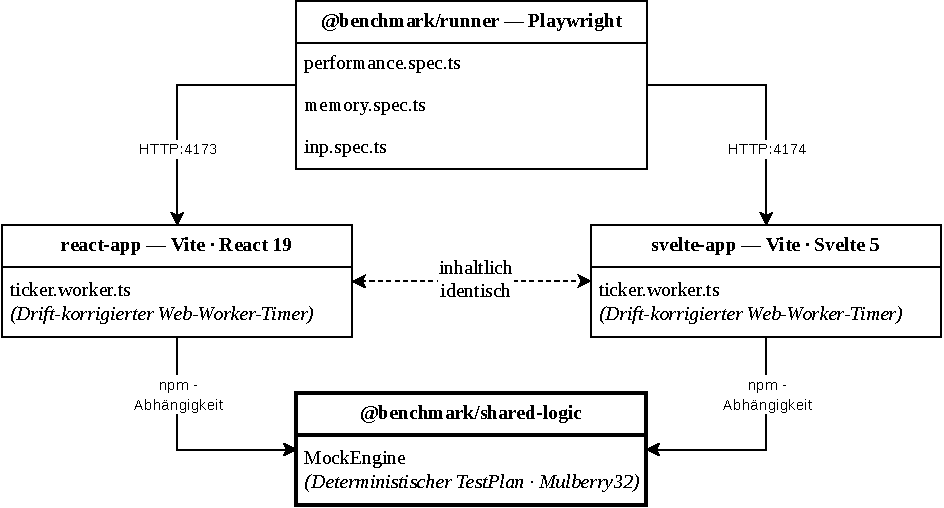
\includegraphics[width=\textwidth]{bilder/diagram_5_1.pdf}
  \caption{Paketstruktur und Abhängigkeitsbeziehungen des npm-Workspace-Monorepos.}
  \label{fig:diagram-5-1}
\end{figure}

\subsection{Das Paket \texttt{@benchmark/shared-logic}}
\label{ss:impl-shared-logic}

Das Paket \texttt{@benchmark/shared-logic} ist als reines TypeScript-Paket ohne Laufzeitabhängigkeiten implementiert; die Kompilierung erfolgt einmalig mit \texttt{tsc}.

\subsection{Datenmodell: Interfaces \texttt{GridItem}, \texttt{TickMutation} und \texttt{TestPlan}}
\label{ss:impl-interfaces}

Das Paket exportiert drei TypeScript-Interfaces, die das Datenmodell beider Anwendungen beschreiben (siehe \cref{lst:interfaces} im Anhang). \texttt{GridItem} repräsentiert eine einzelne Zelle des Grids mit eindeutiger numerischer ID sowie dem aktuellen Anzeigewert. \texttt{TickMutation} beschreibt eine Zustandsänderung einer einzelnen Zelle und spezifiziert deren ID sowie den zugehörigen Folgewert. \texttt{TestPlan} fasst den vollständigen Ablauf eines Szenarios zusammen: \texttt{initialState} enthält den Ausgangszustand aller Zellen, \texttt{ticks} ist ein zweidimensionales Array, dessen äußere Dimension die zeitliche Abfolge der Ticks beschreibt, während die innere Dimension die Zellen angibt, die pro Tick gleichzeitig aktualisiert werden. Der \texttt{TestPlan} entsteht einmalig vor dem ersten Render und bleibt anschließend unverändert (vgl. \cref{sss:mock-engine-validity}).

\subsection{Implementierung der \texttt{MockEngine}}
\label{ss:impl-mockengine}

Die Klasse \texttt{MockEngine} stellt die Methode \texttt{generateTestPlan(gridSize, tickCount, mutationRate, seed\,=\,123)} bereit. Zur Erzeugung deterministischer Zufallswerte kommt der Pseudozufallszahlengenerator Mulberry32 zum Einsatz \cite{ettinger-mulberry32-2017}, da \texttt{Math.random()} keine standardisierte Seed-Initialisierung bietet. Bei gleichem Seed liefert Mulberry32 reproduzierbare Float-Werte im Intervall $[0,1)$. Die Umsetzung auf Basis von 32-Bit-Ganzzahlarithmetik verursacht keinen messbaren Mehraufwand im Benchmark. Die Methode \texttt{generateTestPlan} durchläuft zwei Phasen. In der ersten Phase wird \texttt{initialState} befüllt: Für jede der \texttt{gridSize} Zellen erzeugt Mulberry32 einen Startwert im Bereich $[0, 100)$. Gleichzeitig speichert \texttt{currentValues} in einem Shadow-Array gleicher Länge die aktuellen Zellwerte, die in der zweiten Phase für die Bailout-Guard-Prüfung benötigt werden. In der zweiten Phase entstehen \texttt{tickCount} Tick-Einträge. Die Zahl der je Iteration zu mutierenden Zellen ergibt sich aus $\lceil \mathtt{gridSize} \cdot \mathtt{mutationRate} \rceil$. Die Bestimmung der Indizes erfolgt zufällig und ohne Zurücklegen (vgl. \cref{ss:scenario-a}); hierfür dient ein vorab angelegtes Array aller Zell-Indizes der Länge \texttt{gridSize}, das über alle Ticks hinweg wiederverwendet wird. In jeder Iteration werden nur die ersten \texttt{mutationCount} Positionen des Arrays durch gezielte Tauschoperationen neu angeordnet. Dabei entstehen genau \texttt{mutationCount} eindeutige Indizes ohne Duplikate. Im Vergleich zu einem vollständigen Shuffle mit $O(n)$ reduziert sich der Aufwand je Iteration auf $O(\mathtt{mutationCount})$ \cite{knuth-taocp2-1998}; die Wiederverwendung des Pools vermeidet zudem Heap-Allokationen pro Tick.
Für jeden selektierten Index stellt der Bailout-Guard (vgl. \cref{lst:bailout} im Anhang) sicher, dass der generierte Folgewert nicht mit dem gespeicherten Vorgänger übereinstimmt. Der neue Wert aktualisiert \texttt{currentValues} und gelangt zusammen mit der ID als \texttt{TickMutation} in das entsprechende Tick-Array.

\subsection{Der drift-korrigierte Web-Worker-Timer (\texttt{ticker.worker.ts})}
\label{ss:impl-worker}

Beide Framework-Anwendungen verwenden eine inhaltlich identische Datei \code{ticker.worker.ts}, die als separater Web Worker läuft. Nach dem Empfang einer Startnachricht mit dem gewünschten Tick-Intervall startet er einen Tick-Scheduler, der Drift durch kumulativen Zeitabgleich korrigiert \cite{mills-rfc5905-2010} (vollständiger Code: \cref{lst:worker} im Anhang). Bei jedem Aufruf von \texttt{scheduleNextTick} findet ein Abgleich der realen Ausführungszeit mit \texttt{expectedTime} statt. Die dabei gemessene Abweichung (\texttt{drift}) wird vom nächsten Delay abgezogen, sodass Verspätungen einzelner Ticks in nachfolgenden Intervallen kompensiert werden. Der Worker sendet lediglich ein Zeitsignal. Die eigentlichen Mutationsdaten empfangen die Anwendungen über einen internen Tick-Zähler aus dem vorab berechneten \texttt{TestPlan}. Durch die Ausführung des Workers in einem eigenen Agent-Thread mit separater Event-Loop bleibt die Tick-Frequenz unabhängig von der Rendering-Last des Main Threads \cite{whatwg-html-2026} (vgl. \cref{sss:disturbances}).

\section{Technische Umsetzung der React-Referenzanwendung}
\label{s:impl-react}

Die React-Referenzanwendung ist als Vite-Projekt mit React~19 umgesetzt und besteht aus drei Ebenen: \texttt{App.tsx} bildet den Einstiegspunkt der Anwendung, \texttt{Grid.tsx} übernimmt die Anordnung der Inhalte und \texttt{Cell.tsx} stellt die einzelnen Zellen dar. Dieser Aufbau erfüllt die in \cref{sss:parity} formulierte Anforderung der strukturellen Vergleichbarkeit. Gleichzeitig dient die Anwendung als Grundlage zur Untersuchung des React-Compilers in einer typischen Komponentenstruktur mit geringer Verschachtelungstiefe.

\subsection{Komponentenstruktur und Prop-Weitergabe}
\label{ss:impl-react-components}

Der vollständige \texttt{TestPlan} entsteht in \texttt{App.tsx} bereits auf Modulebene vor der Definition der Komponenten (vgl. \cref{sss:mock-engine-validity}), sodass die Berechnung nur einmal beim Laden des Bundles erfolgt und nicht bei jedem Render-Aufruf. Der Initialzustand des Grids liegt in einem \texttt{useState}-Array vom Typ \texttt{GridItem[]} vor. Darüber hinaus existieren zwei weitere \texttt{useState}-Felder für den Ablaufstatus (\texttt{phase}) und die UI-Fortschrittsanzeige (\texttt{tickCount}). \texttt{App.tsx} gibt das Array als \texttt{items}-Prop an \texttt{Grid.tsx} weiter, das lediglich die Layoutstruktur bereitstellt (vollständiger Komponentencode: \cref{lst:react-grid} im Anhang). 
\noindent\texttt{Grid.tsx} übergibt an \texttt{Cell} den Integer \texttt{value} anstelle des gesamten \texttt{GridItem}-Objekts. Dadurch kann der React-Compiler die Komponente memoisieren und die erneute Ausführung der Renderfunktion vermeiden, solange sich der Wert nicht ändert. Lokale Zustandsänderungen führen weiterhin zu regulären Re-Renders.
Zudem beschränkt sich der Prop-Vergleich des React~Compilers auf einen einfachen Integer-Gleichheitscheck (\texttt{===}), was die strukturelle Vergleichbarkeit mit der Svelte-Implementierung sicherstellt (vgl.~\cref{sss:parity}). \texttt{Cell.tsx} repräsentiert die einzelnen Zellen des Grids. Die Komponente rechnet den übergebenen Wert zur visuellen Hervorhebung in eine Farbe im Farbmodell Hue, Saturation, Lightness (HSL) um. Für den INP-Trigger (vgl.~\cref{sss:inp-trigger}) verwaltet die Komponente zusätzlich einen lokalen \texttt{clicked}-Zustand.

\subsection{Unveränderliche Referenzaktualisierung im Tick-Handler}
\label{ss:impl-react-update}

React erkennt Zustandsänderungen anhand von Objektreferenzen (\cref{ss:vdom}). Der Tick-Handler in \texttt{App.tsx} nutzt dieses Prinzip (vollständiger Code: \cref{lst:react-update} im Anhang): Der Spread-Operator \texttt{[...prev]} erzeugt zunächst eine flache Kopie des Arrays. Für jede der $\lceil n \cdot 0{,}05 \rceil$ mutierten Zellen (vgl.~\cref{ss:scenario-a}) erfolgt anschließend das Einfügen eines neuen \texttt{\{id, value\}}-Objekts an der jeweiligen Position. Alle übrigen Positionen behalten ihre ursprünglichen Objektreferenzen. Diese Eigenschaft ist entscheidend für die Korrektheit der Messung: Da \texttt{Grid} das gesamte \texttt{items}-Array als Prop erhält, löst jede Tick-Mutation ein erneutes Rendering aus. Anschließend vergleicht der React-Compiler für jede \texttt{Cell} den aktuellen \texttt{value}-Prop mit dem zuvor gespeicherten Wert (\texttt{===}) \cite{react_reconcillation_2024}. Nur bei einer Änderung führt die jeweilige Zelle ihre Renderfunktion erneut aus. Abbildung \ref{fig:diagram-5-2-3} zeigt diesen Mechanismus im Vergleich zum Ansatz der direkten Zustandsänderung in Svelte~5. Die flache Kopie des Arrays wirkt sich auch auf die Speicheranalyse aus (\cref{sss:quantitative-heap}): Pro Tick entstehen $\lceil n \cdot 0{,}05 \rceil$ neue \texttt{GridItem}-Objekte sowie ein neues Array der Länge~$n$. Die ersetzten Objekte werden zu Garbage-Collection-Kandidaten.
\begin{figure}[htbp]
  \centering
  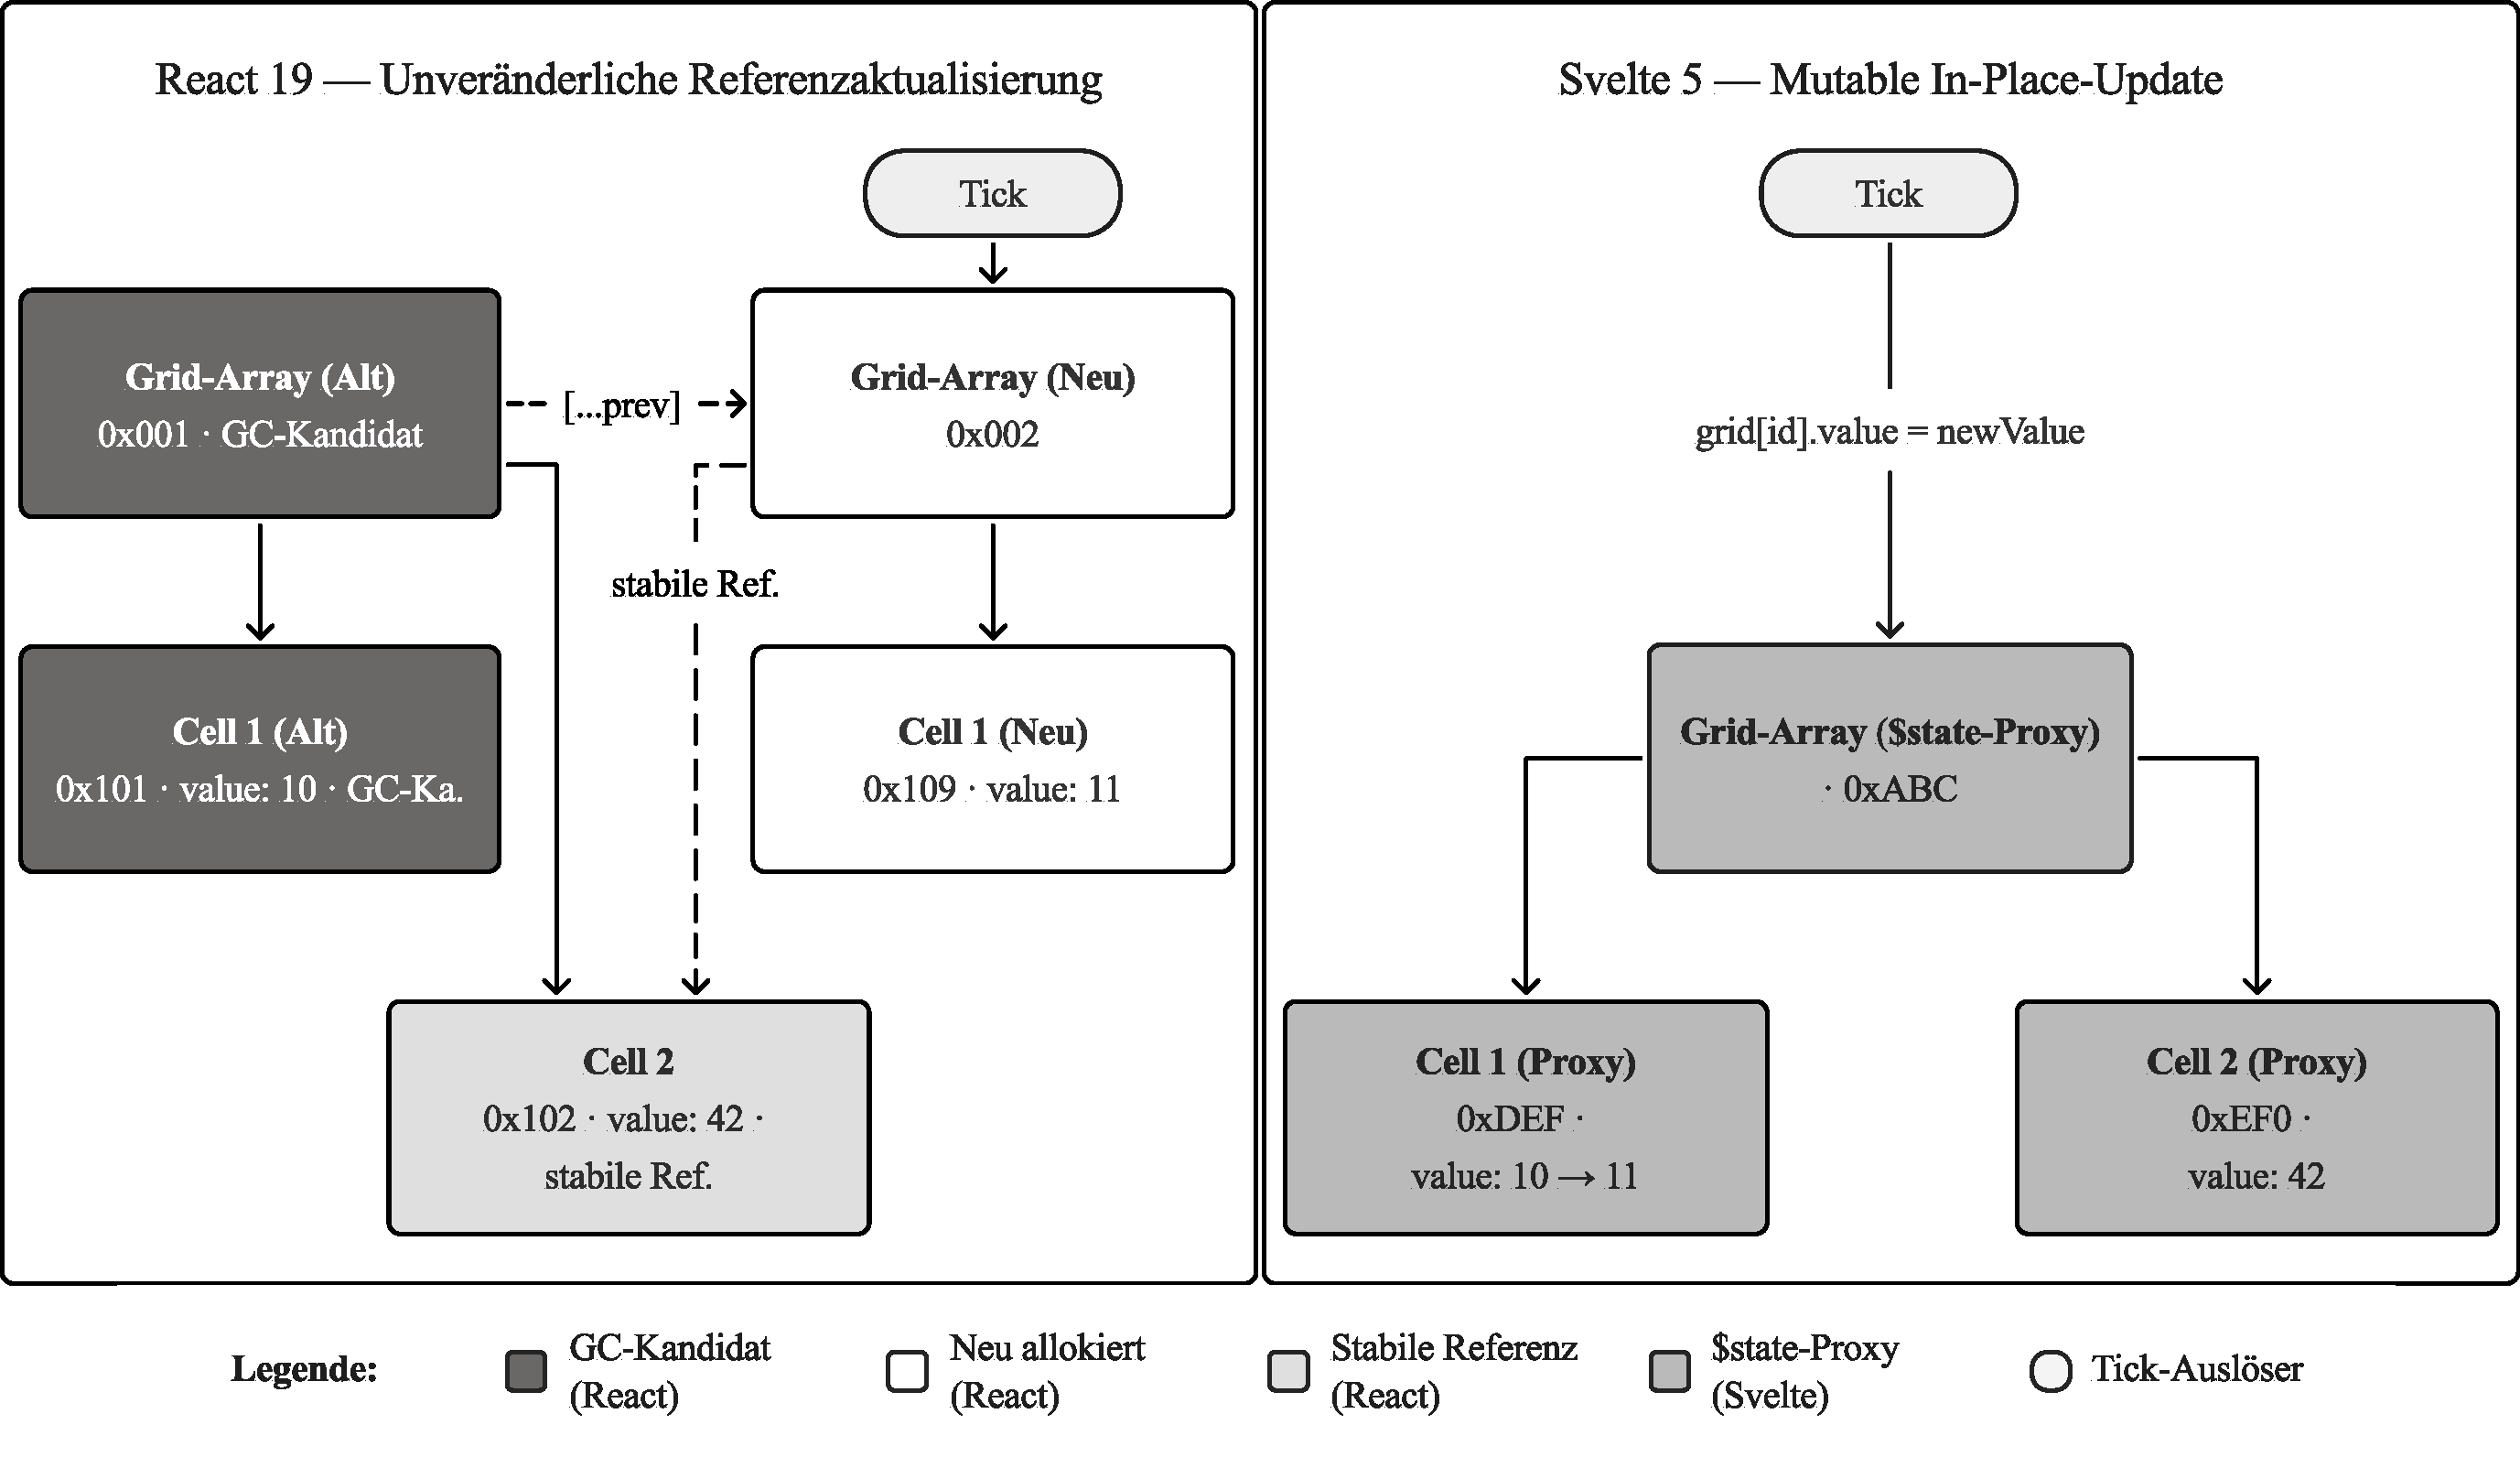
\includegraphics{bilder/diagram_5_2_3.pdf}
  \caption[Gegenüberstellung der Update-Strategien React~19 und Svelte~5]{Gegenüberstellung der Update-Strategien: React~19 arbeitet mit der Erzeugung neuer Heap-Objekte bei jeder Änderung (dunkelgrau markiert als Garbage-Collection-Kandidaten), während Svelte~5 bestehende Signal-Objekte direkt aktualisiert und so zusätzliche Speicherallokationen weitgehend vermeidet (Eigene Darstellung, KI-unterstützt).}
  \label{fig:diagram-5-2-3}
\end{figure}

\subsection{Steuerung durch den Web Worker und Benchmark-Ablauf}
\label{ss:impl-react-worker}

\texttt{App.tsx} instanziiert den Web Worker (\cref{ss:impl-worker}) in einem \texttt{useEffect}-Hook mit leerer Abhängigkeitsliste (\texttt{[]}), sodass die Initialisierung nur einmal nach dem ersten Rendern erfolgt. Zusätzlich registriert der Hook einen \texttt{'benchmark-start'}-Event-Listener auf \texttt{window}. Die vollständige Startlogik ist in \cref{lst:react-lifecycle} im Anhang abgebildet. Das Flag \texttt{IS\_BENCHMARK\_MODE} ist \texttt{true}, sobald der Query-Parameter \texttt{gridSize} in der URL vorhanden ist; andernfalls löst die Anwendung das Ereignis selbst aus und startet unmittelbar. Das \texttt{data-testid}-Attribut des Root-Elements wechselt von \texttt{'benchmark-ready'} auf \texttt{'benchmark-done'}, sobald der Worker beendet wurde und \texttt{setPhase('done')} den zugehörigen React-Re-Render ausgelöst hat (vgl.~\cref{sss:lifecycle}).

\subsection{Integration des React Compilers}
\label{ss:impl-react-compiler}

Die Datei \texttt{vite.config.ts} bindet den React-Compiler als Babel-Plugin in die Build-Pipeline ein (vollständige Konfiguration: \cref{lst:react-compiler-config} im Anhang). Das Plugin \texttt{@vitejs/plugin-react} übernimmt die Standard-Umwandlung von JavaScript XML (JSX), während \texttt{@rolldown/plugin-babel} die anschließende Compiler-Umwandlung ausführt. Die Funktion \texttt{reactCompilerPreset()} bindet \texttt{babel-plugin-react-compiler} als Preset ein und aktiviert es in der in \cref{ss:software-versions} festgelegten Version~1.0.0. Der Compiler analysiert jede Komponente statisch auf Seiteneffekte und veränderte Props. Komponenten ohne solche Eigenschaften werden automatisch memoisiert, sodass das Ergebnis des letzten Renderns zwischengespeichert und eine erneute Ausführung bei unveränderten Eingaben verhindert wird \cite{react_compiler_2025}. Ob der Compiler korrekt aktiv ist, lässt sich auf zwei Ebenen überprüfen. Auf Build-Ebene enthält das erzeugte JavaScript-Bundle typische Compiler-Artefakte, darunter direkte Aufrufe der internen Funktion \texttt{\_c} sowie Zugriffe auf ein Cache-Array, das durch das Symbol \texttt{\$} dargestellt wird. Auf Laufzeitebene kennzeichnet der React DevTools Profiler optimierte Komponenten mit der Annotation \guillemotleft{}Memo\guillemotright{}, wobei ein zusätzliches Sparkle-Symbol anzeigt, dass die Memoisierung automatisch durch den Compiler erfolgte \cite{gsathya-compiler-2024}. Beide Indikatoren sind im vorliegenden Setup erfüllt: Die Komponenten \texttt{App}, \texttt{Grid} und \texttt{Cell} wurden vollständig optimiert. Wie in \cref{sss:forbidden-optimizations} dargelegt, enthält der Quellcode keine manuellen Optimierungen mittels \texttt{React.memo}, \texttt{useMemo} oder \texttt{useCallback}. Zudem hat der \texttt{<StrictMode>}-Wrapper in \texttt{main.tsx} im Production-Build keine Auswirkungen und beeinflusst die Messergebnisse daher nicht (vgl.~\cref{sss:production-build}).

\section{Technische Umsetzung der Svelte-Referenzanwendung}
\label{s:impl-svelte}

Die Umsetzung in Svelte folgt der in \cref{s:impl-react} beschriebenen Dreistufenarchitektur (\texttt{App.svelte}, \texttt{Grid.svelte}, \texttt{Cell.svelte}) und stellt damit die strukturelle Vergleichbarkeit sicher (vgl.~\cref{sss:parity}). Svelte-4-Elemente wie (\texttt{export let}, reaktive Statements \texttt{\$:} und Svelte Stores) kommen nicht zum Einsatz; alle Dateien verwenden ausschließlich die Runes-Syntax von Svelte~5 (vgl.~\cref{sss:forbidden-optimizations}).

\subsection{Komponentenstruktur und Prop-Weitergabe}
\label{ss:impl-svelte-components}

In Svelte~5 gibt es innerhalb einer \texttt{.svelte}-Datei zwei Script-Blöcke: \texttt{<script module>} enthält Code auf Modulebene, der beim Laden genau einmal ausgeführt wird; \texttt{<script>} umfasst instanzbezogenen Code, der bei jedem Mount einer Komponente läuft. In \texttt{App.svelte} kommt diese Trennung gezielt zum Einsatz: Der \texttt{TestPlan} entsteht im \texttt{<script module>}-Block (vgl.~\cref{sss:mock-engine-validity} und \cref{lst:svelte-module} im Anhang), wodurch die Berechnung nicht bei jedem Rendern erneut erfolgt. Das Grid ist im komponentenbezogenen \texttt{<script>}-Block als \texttt{\$state}-Array deklariert (vgl. \cref{lst:svelte-state} im Anhang). Der Spread-Operator \texttt{\{...item\}} erzeugt für jedes \texttt{GridItem}-Objekt eine flache Kopie. Dadurch arbeitet die Anwendung mit eigenen, veränderbaren Instanzen, während der \texttt{TestPlan} selbst unverändert bleibt. \texttt{\$state()} erlaubt es, Änderungen an einzelnen Eigenschaften zur Laufzeit gezielt nachzuverfolgen (vgl.~\cref{sss:finegraned-reactivity}). Die Prop-Weitergabe an \texttt{Grid.svelte} und \texttt{Cell.svelte} erfolgt über die Rune \texttt{\$props()} (vgl. \cref{lst:svelte-props} im Anhang). \texttt{Grid.svelte} iteriert mit einem schlüsselbasierten \texttt{\{\#each\}}-Block und übergibt ausschließlich den primitiven \texttt{value}-Integer an \texttt{Cell}. \texttt{Cell.svelte} verwaltet intern einen \texttt{clicked}-Zustand als \texttt{\$state}. Beide Entscheidungen sind strukturell identisch mit der React-Implementierung (vgl.~\cref{ss:impl-react-components}).

\subsection{Direkte Zustandsmutation im Tick-Handler}
\label{ss:impl-svelte-update}

Der Unterschied liegt in der Art der Zustandsänderung. Anstatt bei jeder Änderung ein neues Array zu erzeugen (vgl.~\cref{ss:impl-react-update}), mutiert Svelte~5 die vorhandenen Objekte direkt (vollständiger Tick-Handler: \cref{lst:svelte-update} im Anhang). Der \texttt{\$state}-Proxy erkennt und verarbeitet die Zuweisung \texttt{grid[id].value = newValue}. Der \texttt{\{\#each\}}-Block in \texttt{Grid.svelte} generiert zur Laufzeit pro Iteration eine feingranulare reaktive Bindung auf \texttt{item.value}. \texttt{Cell.svelte} selbst enthält dabei keine eigene Reaktivitätslogik, sondern empfängt lediglich den aktualisierten primitiven Wert als Prop. Eine Property-Änderung aktualisiert ausschließlich die betroffene \texttt{Cell}, ohne dass das Array kopiert wird, neue Objektreferenzen erzeugt werden oder der gesamte Komponentenbaum durchlaufen wird (vgl.~\cref{sss:finegraned-reactivity}), wodurch die Referenzen auf die einzelnen Objekte in \texttt{grid} während des gesamten Benchmark-Verlaufs stabil bleiben. Reacts \texttt{setGrid}-Aufruf erzeugt hingegen pro Tick neue Objekte und eine neue Array-Instanz (vgl.~\cref{ss:impl-react-update}). Abbildung~\ref{fig:diagram-5-2-3} zeigt diesen Kontrast: React hinterlässt Garbage-Collection-Kandidaten, während Svelte den Heap-Speicherbedarf stabil hält. Dieser strukturelle Unterschied gilt als erwartete Ursache des in Hypothese H3 untersuchten JS-Heap-Deltas (vgl.~\cref{ss:hypotheses}).

\subsection{Steuerung durch den Web Worker und Benchmark-Ablauf}
\label{ss:impl-svelte-worker}

Ein \texttt{\$effect}-Block übernimmt die Instanziierung des Workers (vollständige Implementierung: \cref{lst:svelte-effect} im Anhang). Anders als \texttt{useEffect} in React benötigt \texttt{\$effect} kein Dependency-Array \cite{react_introduction, svelte_migration}, da reaktive Abhängigkeiten automatisch ermittelt werden (vgl.~\cref{ss:svelte-reactivity}). Da dieser Effekt keinen reaktiven State verwendet, besitzt er keine Abhängigkeiten und entspricht somit \texttt{useEffect(fn, [])}; der Rückgabewert ist eine Cleanup-Funktion, die vor jeder erneuten Ausführung sowie beim Unmount der Komponente läuft. Die \texttt{IS\_BENCHMARK\_MODE}-Steuerung und das \texttt{data-testid}-Protokoll sind inhaltlich identisch mit der React-Implementierung (vgl.~\cref{ss:impl-react-worker}). Innerhalb des Tick-Handlers zeigt sich ein weiterer Unterschied: \texttt{tickIndex} ist als \texttt{let tickIndex = 0} nicht reaktiv und löst keine Updates aus. Dieses Verhalten entspricht in React der Verwendung von \texttt{useRef} (\cref{ss:impl-react-update}), stellt in Svelte~5 jedoch den Normalfall dar, da Variablen ohne \texttt{\$state} für das Reaktivitätssystem unsichtbar bleiben. Parallel dazu existiert \texttt{tickCount} als \texttt{\$state}, das ausschließlich den UI-Zähler in der Statuszeile aktualisiert. Diese Trennung macht die Granularität von Sveltes Reaktivitätsmodell sichtbar: Nur explizit deklarierte \texttt{\$state}-Variablen erzeugen Rendering-Arbeit.

\section{Technische Umsetzung des Benchmark-Pakets}
\label{s:impl-benchmark}

Das Paket \texttt{@benchmark/runner} setzt den in \cref{s:automation-and-statistics} beschriebenen automatisierten Testablauf um und speichert die Ergebnisse in einem maschinenlesbaren Format. Es ist in drei voneinander unabhängige Playwright-Testdateien aufgeteilt, von denen jede einen eigenen Messdurchlauf abdeckt: \texttt{performance.spec.ts}, \texttt{memory.spec.ts} und \texttt{inp.spec.ts}. Gemeinsam genutzte Logik liegt in fünf Hilfsmodulen im Verzeichnis \texttt{src/helpers/}: \texttt{scenarios.ts}, \texttt{cdp.ts}, \texttt{longTasks.ts}, \texttt{inp.ts} und \texttt{results.ts}. Die Begründung für die Trennung in drei separate Playwright-Projekte ist in \cref{sss:gc-interference} dargelegt.

\subsection{Playwright-Konfiguration: \texttt{playwright.config.ts}}
\label{ss:impl-playwright-config}

In der Datei \texttt{playwright.config.ts} werden die grundlegenden Konfigurationen für alle drei Projekte festgelegt (vollständige Konfiguration: \cref{lst:playwright-config} im Anhang). \texttt{workers: 1}, \texttt{headless: true} und der Viewport von $1280 \times 720$ Pixeln setzen die in \cref{sss:browser-config} begründeten Anforderungen um. Das Argument \texttt{--disable-software-rasterizer} deaktiviert den SwiftShader-Fallback und stellt sicher, dass Rendering-Arbeit ausschließlich auf den Hardware-GPU-Codepfaden stattfindet, nicht auf CPU-Emulation \cite{chromium-swiftshader}. Auf Maschinen ohne Hardware-GPU lässt sich das Argument über \texttt{NO\_GPU} deaktivieren.

\subsection{Szenariensteuerung: \texttt{scenarios.ts}}
\label{ss:impl-scenarios}

Die Datei \texttt{scenarios.ts} definiert die vollständige Testmatrix als TypeScript-Konstanten. Die Funktion \texttt{allScenarios()} erzeugt durch eine dreifache Schleife über alle Grid-Größen, Frequenzstufen und Frameworks die 64 Szenarien der Testmatrix (\cref{ss:test-matrix}); der vollständige Code findet sich in \cref{lst:scenarios} im Anhang. Jede der drei Spec-Dateien ruft \texttt{allScenarios()} auf und registriert pro Szenario einen \texttt{test()}-Block. Playwright übergibt die Szenariokonfiguration per URL-Query-Parameter an die Anwendungen:
\begin{center}
  \texttt{http://localhost:4173?gridSize=N\&tickInterval=T\&tickCount=C}
\end{center}
Auf diese Weise lässt sich die vollständige Testmatrix ohne Neukompilierung der Anwendungen ausführen (vgl.~\cref{sss:lifecycle}).

\subsection{Performance-Messung: \texttt{performance.spec.ts}}
\label{ss:impl-performance-spec}

\texttt{performance.spec.ts} misst je Szenario die Kennzahlen \textit{scriptingMsPerTick}, \textit{renderingMsPerTick}, \textit{longTaskCount} und \textit{longTaskMs}. Die Synchronisation zwischen Playwright und der Testanwendung basiert auf drei Signalen:

\begin{enumerate}
 \item \texttt{data-testid="benchmark-ready"}: Dieses Attribut kennzeichnet den Initialzustand des Root-Elements beider Anwendungen und ist im DOM sichtbar, sobald der erste Render-Zyklus abgeschlossen ist, d.\,h.\ das Grid vollständig gerendert wurde. Playwright wartet gezielt auf diesen Marker, bevor CDP-Traces gestartet werden. Damit beschränkt sich die Erfassung auf die Rendering-Arbeit des Tick-Loops und schließt das initiale Laden des JavaScript-Bundles sowie das erste Grid-Rendering aus.
 \item \code{window.dispatchEvent(new CustomEvent('benchmark-start'))}: Playwright löst dieses Ereignis nach dem Start der Testumgebung aus. Die Anwendung sendet daraufhin den Startbefehl an den bereits erstellten Web Worker, was den drift-korrigierten (\cref{ss:impl-worker}) Tick-Loop aktiviert (vgl.~\cref{sss:lifecycle}).
 \item \texttt{data-testid="benchmark-done"}: Die Anwendung setzt dieses Attribut nach Abschluss aller Ticks. Playwright nutzt es als eindeutiges Signal für das Ende des Messzeitraums.
\end{enumerate}
Vor dem eigentlichen Messloop erfolgt einmalig ein Warmup-Lauf (vgl.~\cref{sss:jit-interference}), der die V8-JIT-Kompilierung vorab auslöst. Der Ablauf jeder der zehn regulären Messwiederholungen gliedert sich in drei Phasen: Seitenaufruf mit CDP-Session-Aufbau, Start des Long-Task-Beobachters und des CDP-Trace nach \texttt{benchmark-ready}, sowie Auswertung und Ergebnisspeicherung nach \texttt{benchmark-done}. Nach allen zehn Wiederholungen berechnet die Spec für jede der vier Metriken Median und IQR (vgl.~\cref{ss:statistical-evaluation}) und schreibt das Ergebnis als JSON-Datei (vgl.~\cref{ss:impl-results}).

\subsubsection{Long-Task-Beobachter: \texttt{longTasks.ts}}
\label{sss:impl-longtasks}

Die Hilfsfunktion \texttt{injectLongTaskObserver(page)} fügt über \texttt{page.evaluate()} einen \textit{PerformanceObserver} mit \texttt{type: 'longtask'} und \texttt{buffered: false} in den Seitenkontext ein. Durch \texttt{buffered: false} und das \qty{100}{ms}-Delay nach \texttt{benchmark-ready} bleiben Post-Render-Aktivitäten außerhalb des Messfensters (vgl.~\cref{sss:long-task-measurement}). Nach dem Warten auf den \texttt{benchmark-done}-Marker ruft \texttt{collectLongTasks(page)} zunächst \texttt{observer.takeRecords()} auf, um noch nicht asynchron übermittelte Einträge zu sichern \cite{mdn-performance-observer-2024, w3c_longtasks_2026}. Abschließend werden \textit{longTaskCount} und \textit{longTaskMs} berechnet und zurückgegeben.

\subsection{Speichermessung: \texttt{memory.spec.ts}}
\label{ss:impl-memory-spec}

\texttt{memory.spec.ts} bestimmt das JS-Heap-Delta $\Delta_{\mathrm{Heap}}$ gemäß \cref{sss:quantitative-heap}. Analog zu \texttt{performance.spec.ts} erfolgt zunächst ein Warmup-Lauf ohne Messung. Jede Messwiederholung öffnet nach \texttt{page.goto()} eine neue CDP-Session und die Domänen \texttt{HeapProfiler} und \texttt{Performance} aktiviert. Die Funktion \texttt{forceGC(cdp, page)} implementiert die in \cref{sss:gc-interference} beschriebene dreifache GC-Sequenz: drei CDP-Aufrufe von \texttt{HeapProfiler.collectGarbage} mit jeweils \qty{100}{ms} Wartezeit nach jedem Aufruf. Pro Messwiederholung erfolgen zwei Aufrufe von \texttt{forceGC}: nach \texttt{benchmark-ready} zur Erfassung des Heap-Baseline-Werts $H_{\mathrm{base}}$ sowie nach Abschluss aller Ticks vor dem Auslesen des Heap-Endstands $H_{\mathrm{final}}$. Über zehn Wiederholungen ergeben sich Median und IQR des Heap-Deltas $\Delta_{\mathrm{Heap}}$.

\subsection{INP-Messung: \texttt{inp.spec.ts}}
\label{ss:impl-inp-spec}

\texttt{inp.spec.ts} setzt die in \cref{sss:inp-trigger} beschriebene INP-Messung um. Da INP über alle $N=10$ Wiederholungen hinweg gepoolt ist, sammelt die Spec pro Szenario einen gemeinsamen \texttt{allINPEntries}-Puffer.

\subsubsection{INP-Beobachter und Klick-Loop}
\label{sss:impl-inp-observer}

\texttt{injectINPObserver(page)} injiziert über \texttt{page.evaluate()} direkt nach \texttt{page.goto()} einen \textit{PerformanceObserver} in den Seitenkontext. Der Beobachter registriert Events des Typs \texttt{'event'} mit \texttt{durationThreshold: 0}; der browserseitige Mindestschwellenwert von \qty{16}{ms} gilt dennoch \cite{mocny-event-timing-2026}. Für jede erfasste Interaktion werden die drei INP-Phasen berechnet (Formel: \cref{lst:inp-phases} im Anhang). Die Klick-Schleife startet vor dem \texttt{benchmark-start}-Event und führt alle \qty{100}{ms} einen Klick an einer vorab ermittelten Position aus (vgl.~\cref{sss:inp-trigger}).

\subsubsection{INP-Berechnung nach W3C-Spezifikation}
\label{sss:impl-inp-calc}

Die Funktion \texttt{calcINP(allEntries)} setzt die W3C-Spezifikation um (vollständige Implementierung: \cref{lst:inp-calc} im Anhang). Die Einträge werden absteigend nach Dauer sortiert; der schlechteste Wert nach Ausschluss des obersten $\lfloor N/50 \rfloor$-Anteils bildet den INP-Wert (vgl.~\cref{sss:inp-trigger}).

\subsection{CDP-Hilfsfunktionen: \texttt{cdp.ts}}
\label{ss:cdp-helpers}

Die Hilfsfunktion \texttt{startTrace} startet die Aufzeichnung im \texttt{ReportEvents}-Modus und sammelt eingehende Trace-Ereignisse in einem Array. \texttt{stopTrace} beendet die Aufzeichnung und wartet auf das Signal \texttt{Tracing.tracingComplete} \cite{chrome-devtools-tracing}. Die Funktion \texttt{parseTrace(events, tickCount)} ordnet vollständige Trace-Ereignisse anhand ihres Namensfelds den in \cref{ss:profiling-categories} definierten Kategorien zu \cite{chrome-performance-reference-2024}; die Konstantendefinitionen sind in \cref{lst:trace-parse} im Anhang aufgeführt. \texttt{parseTrace} berücksichtigt ausschließlich Ereignisse mit \texttt{ph: 'X'}, bei denen \texttt{cat} den Wert \texttt{'devtools.timeline'} enthält und \texttt{dur} größer null ist. Die Ereignisdauern werden von Mikrosekunden in Millisekunden umgerechnet und mit \texttt{tickCount} normalisiert, was \textit{scriptingMsPerTick} und \textit{renderingMsPerTick} liefert (vgl.~\cref{ss:normalization}).

\subsection{Ergebnisspeicherung und Auswertungsexport: \texttt{results.ts}}
\label{ss:impl-results}

Nach jeder abgeschlossenen Messreihe legt \texttt{saveResult()} die Ergebnisse als formatierte JSON-Datei in einem datumsbasierten Verzeichnis (\texttt{results/YYYY-MM-DD/}) ab. Der Dateiname enthält Informationen zu Metrik, Framework, Grid-Größe und Tick-Intervall, beispielsweise \texttt{perf\_react\_n1600\_f50.json}. Die Performance- und Speicher-Dateien enthalten neben Median und IQR je Metrik auch die Rohdaten aller Einzelwiederholungen, sodass die statistische Auswertung im Nachhinein nachvollziehbar ist. INP-Dateien speichern ausschließlich das Ergebnis (\texttt{INPResult}); da die Einträge aller Wiederholungen vor der Berechnung zu einem gemeinsamen Pool zusammengeführt werden, liegen keine separaten Wiederholungswerte vor. Nach Abschluss aller drei Benchmark-Läufe führt \texttt{writeSummaryCSV(dateStr)} die einzelnen JSON-Dateien anhand des im Dateinamen enthaltenen Szenario-Bezeichners (\texttt{framework\_nN\_fT}) in einer \texttt{summary.csv} zusammen. Pro Zeile enthält diese die sechs Primärmetriken eines Szenarios. Die Performance-Metriken \textit{scriptingMsPerTick}, \textit{renderingMsPerTick}, \textit{longTaskCount} und \textit{longTaskMs} liegen jeweils als Median und IQR vor; das Heap-Delta \textit{heapDelta} ausschließlich als Median (\texttt{heapDelta\_median\_bytes}). INP wird als einzelner W3C-Wert exportiert, ergänzt um die Phasenwerte sowie die Anzahl der berücksichtigten Einträge (\textit{pooledEntries}). Die \texttt{summary.csv} dient als Grundlage für die statistische Auswertung in \cref{ch:results}.

\chapter{Ergebnisse und Auswertung}
\label{ch:results}

Alle 1920 Benchmark-Läufe der in \cref{ss:test-matrix} definierten Testmatrix wurden erfolgreich abgeschlossen; kein einzelner Lauf musste verworfen werden. Sämtliche im Folgenden genannten Messwerte sind, sofern nicht durch eine eigene Abbildung oder Tabelle im Fließtext belegt, in \cref{tab:appendix-benchmark} im Anhang vollständig dokumentiert. Ab $n = 8000$ ist die Messstreuung (IQR) in mehreren Szenarien sichtbar erhöht. Als wahrscheinlichste Ursache kommen die Browser-internen Störeinflüsse (\cref{sss:gc-interference,sss:jit-interference}) in Betracht, die sich nicht vollständig kontrollieren lassen.

\section{H2: Scripting-Aufwand pro Tick bei steigender UI-Dichte}
\label{s:results-h2}

\subsection{Scripting-Zeit, Overhead-Faktor und Frequenzeinfluss}
\label{ss:results-h2-scripting}

Mit zunehmender UI-Dichte~$n$ steigen die medianen \textit{scriptingMsPerTick}-Werte beider Frameworks stetig an (\cref{fig:h2-scripting}a). Die Kurve von React verläuft dabei durchgehend steiler als die von Svelte; bei $n = 10\,000$ und $f = 10\,\text{Hz}$ beträgt die Scripting-Zeit für React $11{,}2\,\text{ms}$ gegenüber $4{,}1\,\text{ms}$ für Svelte. Ab $n \geq 8000$ erhöht sich die Messstreuung (IQR) deutlich, was auf die in \cref{sss:gc-interference,sss:jit-interference} diskutierten browserinternen Störeinflüsse zurückgeführt werden kann. Der in \cref{fig:h2-scripting}b gezeigte Overhead-Faktor (Verhältnis von React- zu Svelte-Scripting-Zeit) wächst bei $f = 10\,\text{Hz}$ mit zunehmendem~$n$: Der relative Scripting-Mehraufwand von React gegenüber Svelte nimmt mit steigender UI-Dichte zu. Beide Frameworks weisen zwar eine Skalierung von $O(n)$ auf (\cref{ss:expected-scaling,sss:runes-overhead}), unterscheiden sich jedoch im Aufwand pro Element. Reacts Reconciliation verarbeitet bei jeder Zustandsänderung stets den gesamten betroffenen Teilbaum, unabhängig davon, wie viele Knoten tatsächlich verändert wurden (\cref{ss:expected-scaling}). Zusätzlich werden bei jedem Render-Vorgang erneut React-Elemente erzeugt. Sveltes feingranulare Reaktivität begrenzt den Aufwand hingegen auf die tatsächlich betroffenen Abhängigkeiten (\cref{sss:finegraned-reactivity}), was den Aufwand pro Element reduziert (\cref{sss:runes-overhead}). Für $f = 10\,\text{Hz}$ weisen beide Frameworks bei jeder $n$-Stufe nahezu identische Rendering-Zeiten auf: Bei $n = 4000$ erreichen beide $4{,}74\,\text{ms}$ pro Tick; bei $n = 10\,000$ betragen die Werte $13{,}31\,\text{ms}$ (React) gegenüber $13{,}55\,\text{ms}$ (Svelte, Abweichung $1{,}8\,\%$). Der messbare Unterschied zwischen den Frameworks liegt bei dieser Frequenz somit überwiegend im Scripting (\cref{ss:profiling-categories}). Die INP-Phasenzerlegung (\cref{ss:results-h1-phases}) zeigt bei $f = 10\,\text{Hz}$ allerdings einen deutlichen Unterschied in der \textit{presentationDelay} ($51{,}9\,\text{ms}$ vs.\ $78{,}1\,\text{ms}$). Dieser Unterschied wird durch die Rendering-Zeit pro Tick nicht erfasst; die Ursache lässt sich mit den erhobenen Metriken nicht eindeutig bestimmen (vgl.~\cref{s:limitations}). Bei $f = 20\,\text{Hz}$ treten jedoch Unterschiede auf: Für $n = 10\,000$ betragen die Rendering-Zeiten $11{,}87\,\text{ms}$ (React) beziehungsweise $13{,}71\,\text{ms}$ (Svelte), was einer Abweichung von $15\,\%$ entspricht. Als mögliche Ursache kommt Sveltes Effect-Batching in Betracht (\cref{sss:microtasks}): Die gebündelten DOM-Updates werden innerhalb eines einzigen Microtasks abgearbeitet, ohne dass verbleibende Arbeit auf spätere Frames verteilt wird (\cref{sss:scheduling-priotising-of-updates}). Dadurch könnte der Rendering-Aufwand bei $f = 20\,\text{Hz}$ pro Tick gebündelt anfallen. React hingegen gibt durch kooperatives Yielding (\cref{sss:scheduling-priotising-of-updates}) die Kontrolle zwischen einzelnen Fiber-Schritten an den Browser zurück. Der genaue Mechanismus lässt sich anhand der vorliegenden Daten nicht eindeutig bestimmen. Der Rendering-Unterschied ist bei $f = 20\,\text{Hz}$ am größten ($15\,\%$) und gleicht sich bei $f \approx 62\,\text{Hz}$ nahezu aus ($4{,}95\,\text{ms}$ vs.\ $4{,}92\,\text{ms}$). Mit steigender Tick-Frequenz nimmt die Scripting-Zeit pro Tick insgesamt ab, jedoch nicht gleichförmig und nicht gleich stark bei beiden Frameworks. Bei Svelte steigt die Scripting-Zeit bei $n = 10\,000$ von $4{,}12\,\text{ms}$ ($10\,\text{Hz}$) zunächst auf $4{,}29\,\text{ms}$ ($20\,\text{Hz}$) an, bevor sie auf $3{,}66\,\text{ms}$ ($62\,\text{Hz}$) fällt. Für React ($n = 10\,000$) fällt \textit{scriptingMsPerTick} von $11{,}2\,\text{ms}$ ($10\,\text{Hz}$) auf $3{,}42\,\text{ms}$ ($62\,\text{Hz}$): ein Rückgang um $70\,\%$. Für Svelte sinkt der Wert im selben Bereich von $4{,}1\,\text{ms}$ auf $3{,}66\,\text{ms}$ (Rückgang um $11\,\%$). Beide Frameworks nähern sich mit steigender Frequenz einem gemeinsamen Mindestaufwand an: dem durch die $O(n)$-Komplexität bedingten Basisaufwand, den keine Laufzeitoptimierung unterschreiten kann ($\lceil n \cdot 0{,}05 \rceil$ Signal-Auswertungen bzw.\ die Fiber-Reconciliation, vgl.\ \cref{sss:runes-overhead}). Da Reacts Ausgangswert bei niedrigen Frequenzen weiter von diesem Minimum entfernt liegt als der von Svelte, fällt der relative Rückgang für React entsprechend größer aus. Der große React-Rückgang deutet auf frequenzabhängig wegfallenden Overhead hin, möglicherweise durch JIT-Optimierungen auf häufig ausgeführten Code-Pfaden (\cref{sss:jit-interference}). Sveltes geringer Rückgang ergibt sich daraus, dass der Spielraum nach unten von vornherein klein ist. Der genaue Mechanismus lässt sich ohne V8-internes Profiling nicht bestimmen. Bei $f \approx 62\,\text{Hz}$ und $n = 10\,000$ ergibt sich dadurch ein Scripting-Schnittpunkt: React erreicht $3{,}42\,\text{ms}$ (IQR $0{,}13\,\text{ms}$), Svelte $3{,}66\,\text{ms}$ (IQR $0{,}10\,\text{ms}$); damit ist Svelte hier erstmals geringfügig langsamer als React. Auffällig ist, dass Reacts Scripting-Zeit bei $f \approx 62\,\text{Hz}$ von $n = 8000$ ($3{,}53\,\text{ms}$) auf $n = 10\,000$ ($3{,}42\,\text{ms}$) leicht zurückgeht, während sie bei allen anderen Frequenzen durchgehend mit~$n$ wächst. Da der Unterschied von $0{,}11\,\text{ms}$ kleiner ist als der IQR beider Messpunkte ($n = 8000$: $0{,}20\,\text{ms}$; $n = 10\,000$: $0{,}13\,\text{ms}$), lässt er sich nicht sicher vom Messrauschen unterscheiden. Der Scripting-Schnittpunkt ergibt sich daher überwiegend aus Sveltes $O(n)$-Angleichung (\cref{sss:runes-overhead}) und dem ungleichmäßigen frequenzabhängigen Rückgang im Scripting, nicht dadurch, dass Reacts Scripting-Zeit gestiegen wäre. Damit schränkt der Scripting-Schnittpunkt H2 ein, ohne H2 zu widersprechen. Die Rendering-Zeiten verlaufen bei $n = 10\,000$ uneinheitlich. Bereits bei $f = 10\,\text{Hz}$ sind sie nahezu identisch. Nach dem Maximum des Abstands bei $f = 20\,\text{Hz}$ fallen die React-Werte stetig: von $13{,}31\,\text{ms}$ ($10\,\text{Hz}$) über $11{,}87\,\text{ms}$ ($20\,\text{Hz}$) und $8{,}40\,\text{ms}$ ($30\,\text{Hz}$) auf $4{,}95\,\text{ms}$ ($62\,\text{Hz}$). Sveltes Werte bleiben zunächst bei $13{,}55\,\text{ms}$ ($10\,\text{Hz}$) bzw. $13{,}71\,\text{ms}$ ($20\,\text{Hz}$), bevor sie über $9{,}45\,\text{ms}$ ($30\,\text{Hz}$) auf $4{,}92\,\text{ms}$ ($62\,\text{Hz}$) abfallen. Bei $f \approx 62\,\text{Hz}$ nähern sich beide Frameworks einem gemeinsamen Wert von ca. $4{,}9\,\text{ms}$ an. Der genaue Mechanismus dieser frequenzabhängigen Abnahme lässt sich anhand der vorliegenden Messdaten nicht eindeutig bestimmen.
\begin{figure}[H]
  \centering
  \begin{minipage}[t]{\textwidth}
    \centering
    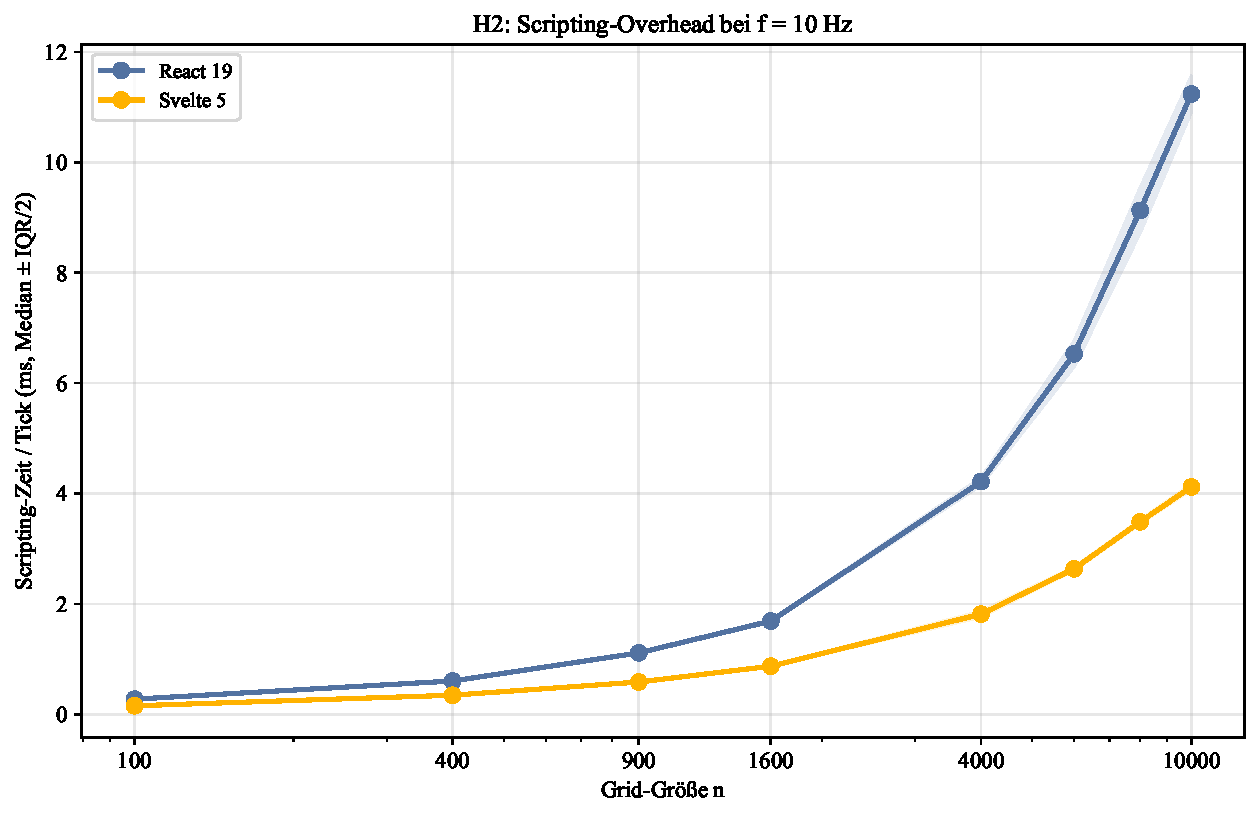
\includegraphics[width=\textwidth,keepaspectratio]{bilder/h2_scripting}
    \subcaption{Scripting-Zeit (Median\,±\,IQR) bei $f = 10\,\text{Hz}$}
    \label{fig:h2-scripting-abs}
  \end{minipage}
  \vspace{1.5em}
  \begin{minipage}[t]{\textwidth}
    \centering
    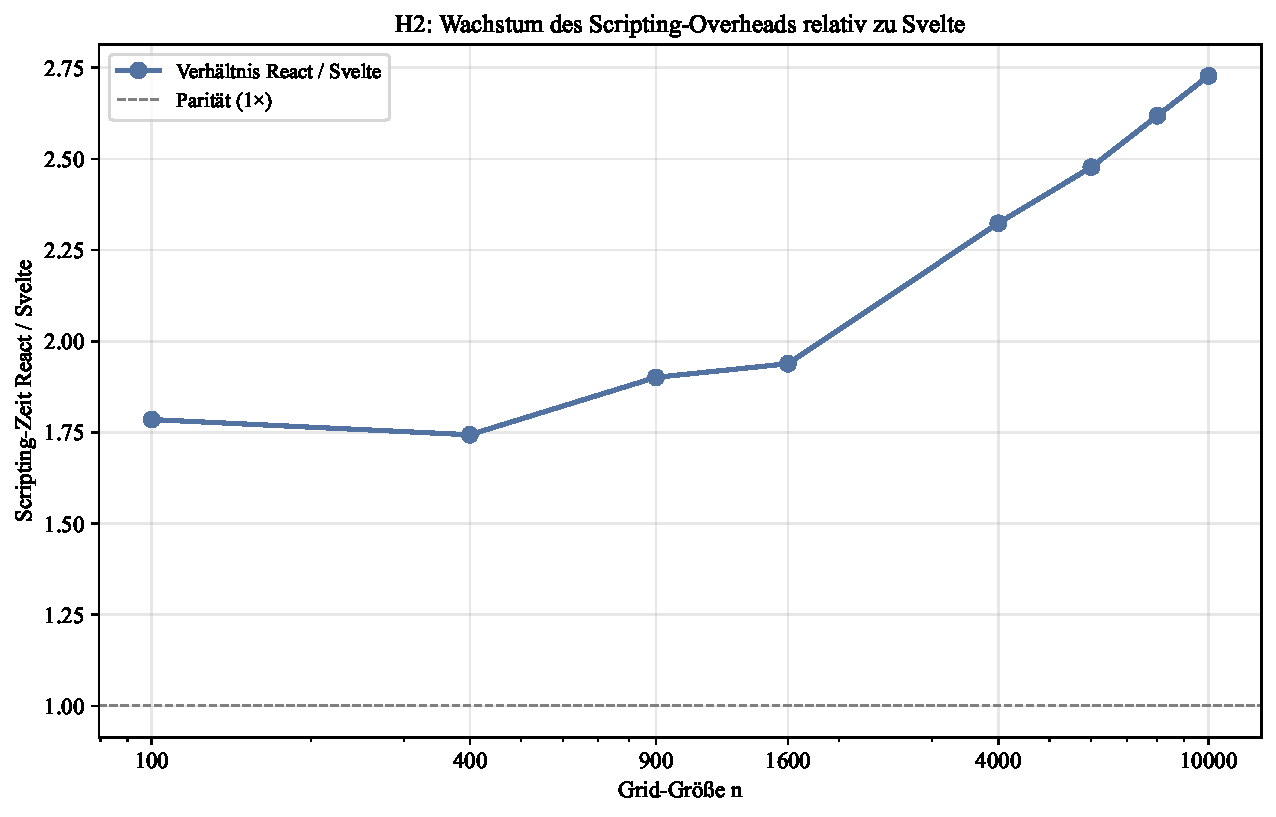
\includegraphics[width=\textwidth,keepaspectratio]{bilder/h2_scripting_ratio}
    \subcaption{Overhead-Faktor React\,/\,Svelte über $n$ bei $f = 10\,\text{Hz}$}
    \label{fig:h2-scripting-ratio}
  \end{minipage}
  \caption[H2 – Scripting-Auswertung beider Frameworks bei $f = 10\,\text{Hz}$]{H2 – Scripting-Auswertung: (a) mediane \textit{scriptingMsPerTick} beider
           Frameworks bei $f = 10\,\text{Hz}$; (b) Quotient React\,/\,Svelte bei
           $f = 10\,\text{Hz}$ über alle $n$-Stufen (vgl.~\cref{ss:profiling-categories}).}
  \label{fig:h2-scripting}
\end{figure}

\subsection{Bewertung von H2}
\label{ss:results-h2-verdict}

Bei $f \leq 30\,\text{Hz}$ bestätigen die Messdaten H2: Der Scripting-Aufwand pro Tick von React wächst mit steigendem~$n$ stärker als der von Svelte, was auf die Reconciliation-Kosten der Fiber-Architektur und die feingranulare Reaktivität von Svelte zurückzuführen ist (\cref{sss:fiber-engine-structure,sss:runes-overhead}). Anzumerken ist, dass sich der genaue Anteil der Compiler-Memoisierung an diesen Scripting-Kosten im gewählten Versuchsaufbau nicht isolieren lässt (vgl.~\cref{s:limitations}). Hinzu kommt, dass bei $f \approx 30\,\text{Hz}$ der Abstand im letzten $n$-Intervall ($n = 8000$ auf $n = 10\,000$) von $3{,}94\,\text{ms}$ auf $3{,}35\,\text{ms}$ zurückgeht: Sveltes Scripting-Zuwachs ($+0{,}79\,\text{ms}$) übersteigt dort den von React ($+0{,}20\,\text{ms}$). Da der Unterschied von $0{,}59\,\text{ms}$ jedoch innerhalb der Summe der IQR-Werte beider Frameworks bei $n = 8000$ liegt (React-IQR: $0{,}40\,\text{ms}$, Svelte-IQR: $0{,}19\,\text{ms}$), lässt er sich nicht sicher vom Messrauschen unterscheiden. Bei $f \approx 62\,\text{Hz}$ gilt H2 nur eingeschränkt: Svelte erreicht bei $n = 10\,000$ mit $3{,}66\,\text{ms}$ erstmals eine höhere Scripting-Zeit als React ($3{,}42\,\text{ms}$). Dieser Scripting-Schnittpunkt lässt sich durch zwei Faktoren erklären: die in \cref{sss:runes-overhead} beschriebene $O(n)$-Angleichung, die bei steigendem $n$ auch bei einer Mutationsrate von $5\,\%$ je Tick praktisch wirksam wird, sowie den ungleichmäßigen frequenzabhängigen Scripting-Rückgang (\cref{ss:results-h2-scripting}). \textbf{H2 wird teilweise bestätigt.}

\section{H3: Speichereffizienz unter Dauerlast}
\label{s:results-h3}

\subsection{Qualitative Heap-Analyse: Dominator-Struktur im Dev-Build}
\label{ss:results-h3-qualitative}

Heap-Snapshots bei $n = 100$ im Development-Build zeigen die internen Datenstrukturen beider Frameworks in lesbarer Form (\cref{sss:qualitative-heap}). \Cref{fig:heap-structures} stellt die aufgeklappten Objekte gegenüber; \cref{tab:heap-qualitative} fasst die abgelesenen Größen zusammen.
\begin{table}[htbp]
  \centering
  \caption[Qualitative Heap-Analyse: interne Objekt-Strukturen ($n = 100$, Dev-Build)]{Qualitative Heap-Analyse: interne Objekt-Strukturen bei $n = 100$
           im Development-Build (Chrome DevTools, Heap-Snapshot nach
           Benchmark-Abschluss)}
  \label{tab:heap-qualitative}
  \small
  \begin{tabular}{lrr}
    \toprule
    \textbf{Metrik}
      & \textbf{React 19} (\texttt{FiberNode})
      & \textbf{Svelte 5} (Signal-POJO) \\
    \midrule
    Instanzen ($n = 100$)  &  423      &  103      \\
    Shallow Size gesamt    & 60{,}9\,kB &  5{,}8\,kB \\
    Retained Size gesamt   & 131\,kB   & 19{,}8\,kB \\
    \bottomrule
  \end{tabular}
  \par\smallskip
  \raggedright\footnotesize
  \textit{Anmerkung:} Shallow Size pro Objekt (berechnet als Gesamt\,÷\,Anzahl):
  React $\approx 144$\,B, Svelte\,5 $\approx 56$\,B.
  Quelle: Chrome DevTools Memory-Tab, Summary-Ansicht, Dev-Build
  (\texttt{localhost:5173} bzw.\ \texttt{localhost:5174}, \texttt{gridSize=100}).
\end{table}
\begin{figure}[H]
  \centering
  \begin{subfigure}{\textwidth}
    \centering
    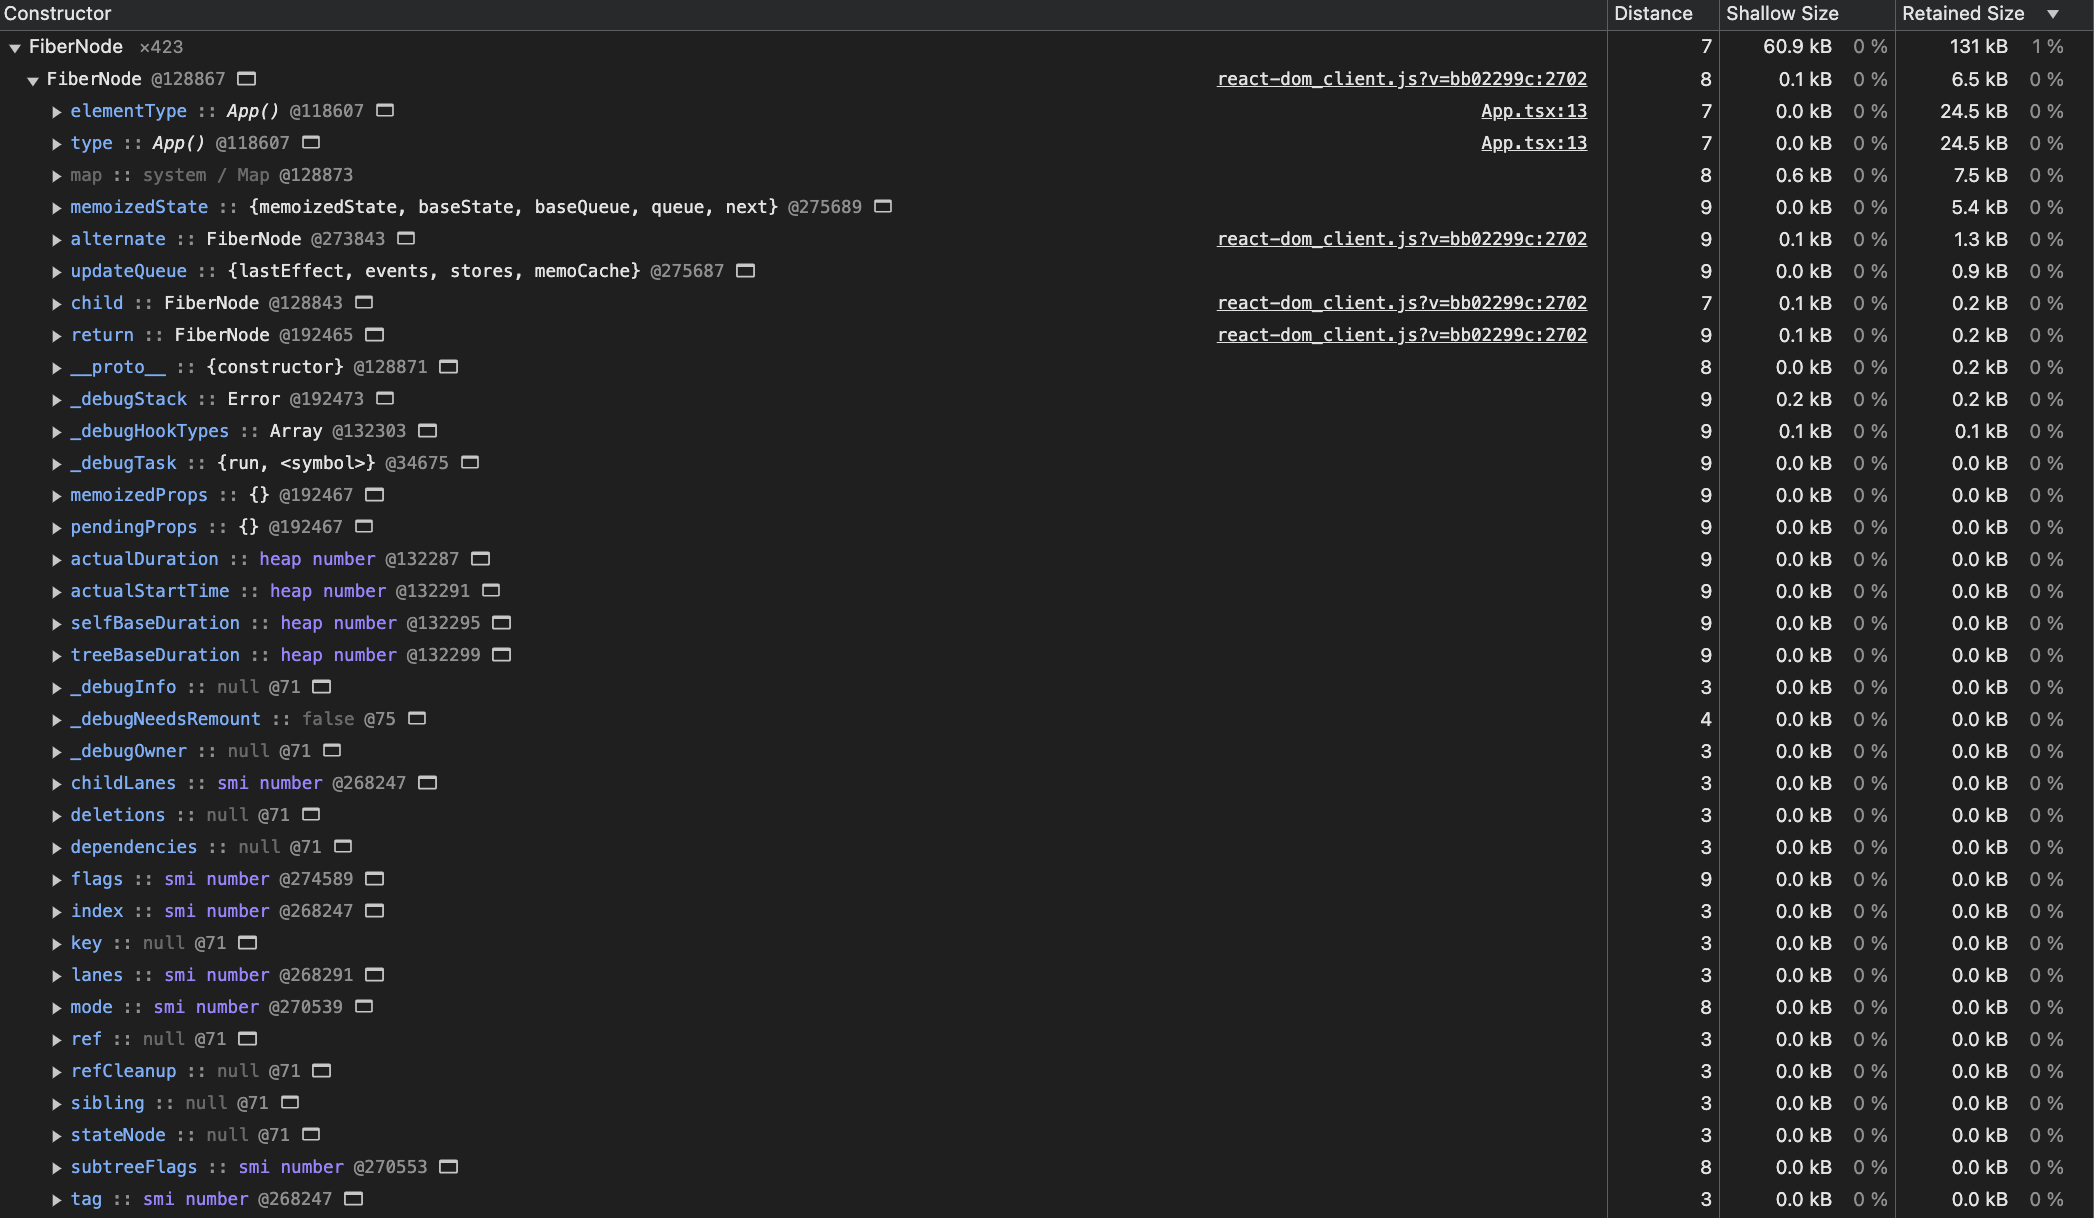
\includegraphics[width=\textwidth]{bilder/heap-react-fibertree}
    \subcaption{React 19: \texttt{FiberNode}-Instanz mit allen Feldern}
    \label{fig:heap-react}
  \end{subfigure}
  \vspace{0.5em}
  \begin{subfigure}{\textwidth}
    \centering
    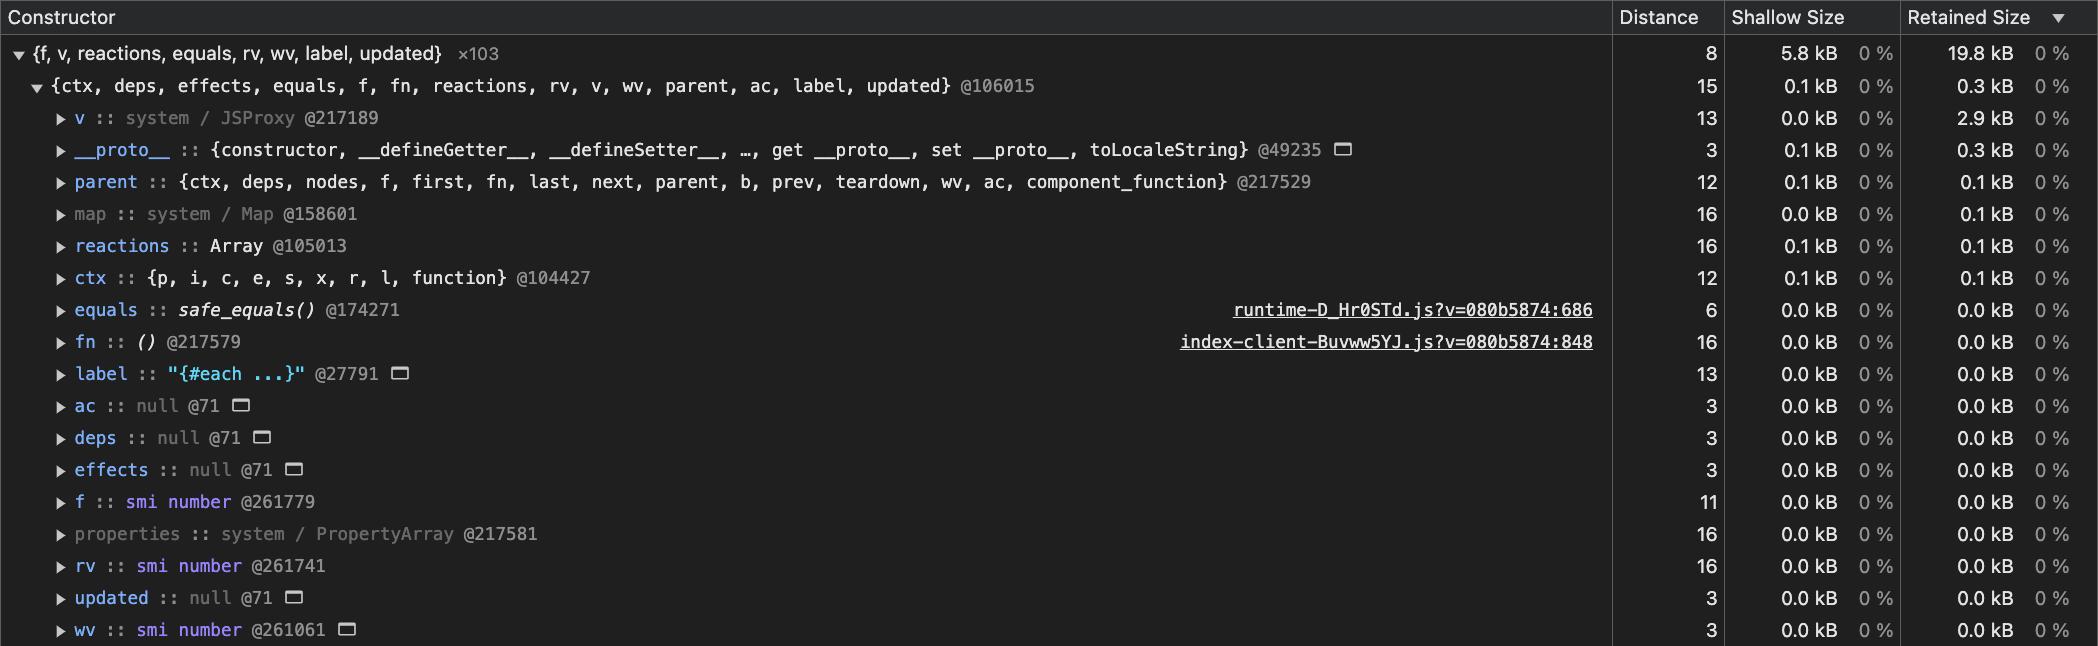
\includegraphics[width=\textwidth]{bilder/heap-svelte-signal}
    \subcaption{Svelte 5: Signal-POJO \texttt{\{f, v, reactions, \ldots\}}}
    \label{fig:heap-svelte}
  \end{subfigure}
  \caption[Chrome DevTools Heap-Snapshot ($n = 100$, Dev-Build): interne Objekte im Vergleich]{Chrome DevTools Heap-Snapshot ($n = 100$, Dev-Build):
           aufgeklappte interne Objekte beider Frameworks im Vergleich.
           Reacts \texttt{FiberNode} enthält neben Produktionsfeldern
           neun ausschließlich im Dev-Build vorhandene Debug-Felder
           (\texttt{\_debugStack}, \texttt{actualDuration} u.\,a.),
           während Sveltes Signal-POJO auf acht Felder beschränkt ist;
           die Feldanzahlen sind in (a) und (b) direkt ablesbar
           (Architekturkontext: \cref{sss:fiber-engine-structure,sss:runes-overhead}).}
  \label{fig:heap-structures}
\end{figure}

\newpage
\subsection{JS-Heap-Delta und Speicher-Overhead-Verhältnis}
\label{ss:results-h3-scaling}

Das JS-Heap-Delta $\Delta_{\mathrm{Heap}}$ wächst bei React über alle $n$-Stufen deutlich stärker als bei Svelte (\cref{fig:h3-memory}a). Beide Kurven steigen stetig mit~$n$. Der Abstand zwischen den Frameworks nimmt dabei mit zunehmendem $n$ zu. Der Frequenzeinfluss auf $\Delta_{\mathrm{Heap}}$ ist vernachlässigbar: Der React-Wert beträgt ca. $4450\,\text{kB}$ ($f = 10\,\text{Hz}$) bzw. ca. $4830\,\text{kB}$ ($f \approx 62\,\text{Hz}$) bei $n = 10\,000$. Der in \cref{fig:h3-memory}b gezeigte Speicher-Overhead-Faktor liegt bei $n = 100$ bei $2{,}8\times$ und erreicht bei $n = 6000$ ein Maximum von $6{,}4\times$. Dieser Anstieg lässt sich durch die in \cref{ss:results-h3-qualitative} ermittelte Retained Size der \texttt{FiberNode}-Instanzen erklären: React benötigt pro Komponenteninstanz erheblich mehr Speicher als Sveltes Signal-POJOs (vgl. \cref{sss:runes-overhead}). Auffällig ist, dass der Overhead-Faktor nach dem Maximum ($n = 6000$: $6{,}37\times$) nicht weiter ansteigt, sondern für größere $n$ wieder abnimmt ($n = 8000$: $6{,}24\times$, $n = 10\,000$: $6{,}18\times$; zuvor $n = 4000$: $5{,}92\times$). Diese Abflachung ab $n = 6000$ lässt sich anhand der vorliegenden Daten nicht eindeutig begründen und wird daher lediglich dokumentiert.
\begin{figure}[H]
  \centering
  \begin{minipage}[t]{\textwidth}
    \centering
    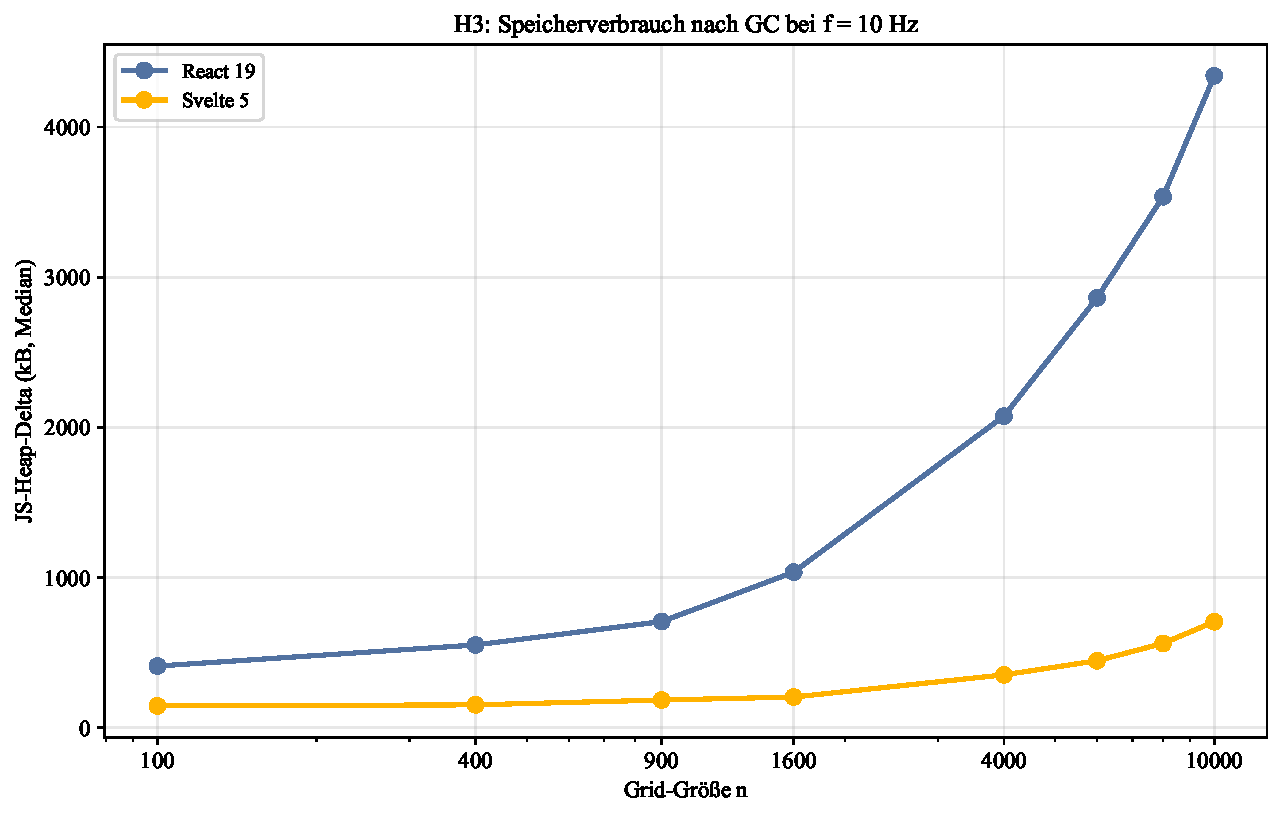
\includegraphics[width=\textwidth,keepaspectratio]{bilder/h3_memory}
    \subcaption{JS-Heap-Delta ($\Delta_{\mathrm{Heap}}$, in kB) bei $f = 10\,\text{Hz}$}
    \label{fig:h3-memory-abs}
  \end{minipage}
  \vspace{1.5em}
  \begin{minipage}[t]{\textwidth}
    \centering
    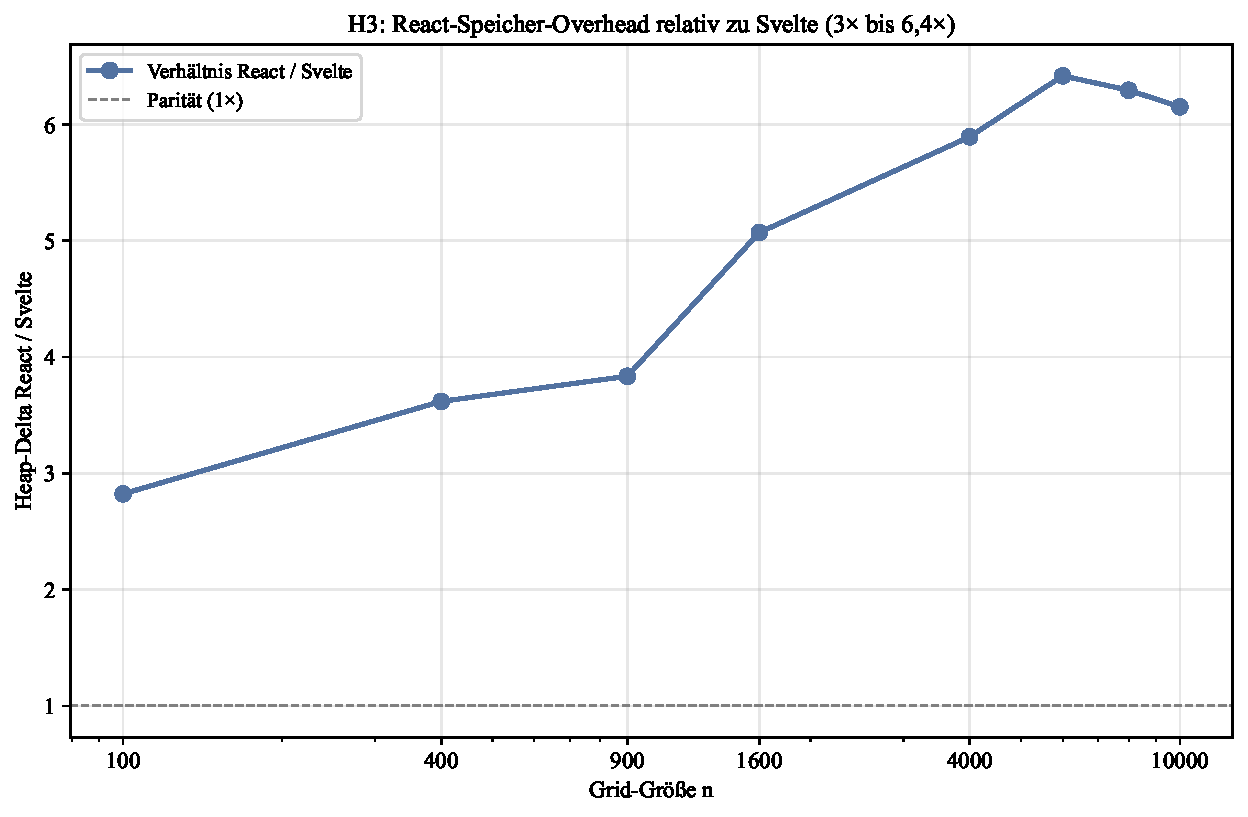
\includegraphics[width=\textwidth,keepaspectratio]{bilder/h3_memory_ratio}
    \subcaption{Speicher-Overhead-Faktor React\,/\,Svelte über $n$ bei $f = 10\,\text{Hz}$}
    \label{fig:h3-memory-ratio}
  \end{minipage}
  \caption[H3 – Speicherauswertung: JS-Heap-Delta beider Frameworks bei $f = 10\,\text{Hz}$]{H3 – Speicherauswertung: (a) medianes JS-Heap-Delta beider Frameworks
           bei $f = 10\,\text{Hz}$; (b) Quotient React\,/\,Svelte bei
           $f = 10\,\text{Hz}$ über alle $n$-Stufen (vgl.~\cref{ss:memory-efficiency}).}
  \label{fig:h3-memory}
\end{figure}

\subsection{Bewertung von H3}
\label{ss:results-h3-verdict}

H3 formuliert die Hypothese bezogen auf die Retained Size pro Komponente (\cref{ss:hypotheses}); diese ist in \cref{ss:results-h3-qualitative} qualitativ bestätigt: Bei $n = 100$ beträgt die Retained Size gesamt React $131\,\text{kB}$ vs. Svelte $19{,}8\,\text{kB}$ (vgl.~\cref{tab:heap-qualitative}), entspricht ${\approx}1{,}31\,\text{kB}$ vs. ${\approx}0{,}20\,\text{kB}$ pro Komponente: Faktor ${\approx}6{,}6\times$. Da der \texttt{FiberNode} im Development-Build neun zusätzliche Debug-Felder enthält (\cref{fig:heap-structures}), die im Production-Build nicht vorhanden sind, ist das gemessene Verhältnis gegenüber dem Production-Build nach oben verzerrt. Das JS-Heap-Delta $\Delta_{\mathrm{Heap}}$ misst die Skalierung quantitativ über alle $n$-Stufen im Production-Build (\cref{sss:quantitative-heap}) und bildet damit die belastbarere Vergleichsbasis für H3. React weist über alle $n$-Stufen einen deutlich höheren Speicherverbrauch auf als Svelte; der Overhead reicht von $2{,}8\times$ ($n = 100$) bis $6{,}4\times$ ($n = 6000$). Die Richtung dieses Faktors ist konsistent mit den im Development-Build beobachteten Unterschieden in der Retained Size der internen Datenstrukturen (\cref{ss:results-h3-qualitative}). Die dort ermittelten konkreten Verhältniswerte sind jedoch nicht direkt auf den Production-Build übertragbar. Die beobachtete Abflachung des Overhead-Faktors ab $n = 6000$ weicht zwar vom erwarteten Wachstum ab, steht jedoch nicht im Widerspruch zu H3. \textbf{H3 wird bestätigt.}

\section{H1: Interaktionslatenz (INP) unter Last}
\label{s:results-h1}

\subsection{INP-Verlauf über die Grid-Größe}
\label{ss:results-h1-curves}

\Cref{fig:h1-inp} zeigt den INP beider Frameworks bei $f = 10\,\text{Hz}$ und $f \approx 62\,\text{Hz}$ über alle $n$-Stufen. Der maximale gemessene INP beträgt $144\,\text{ms}$ (React, $n = 10\,000$, $f \approx 62\,\text{Hz}$) und liegt damit durchgängig im Bereich „Good" ($\leq 200\,\text{ms}$) der Web-Vitals-Klassifikation (\cref{ss:inp}). Dennoch steigt der INP beider Frameworks mit wachsender UI-Dichte spürbar an; React erreicht in der Mehrzahl der Szenarien höhere Werte als Svelte.
\begin{figure}[H]
  \centering
  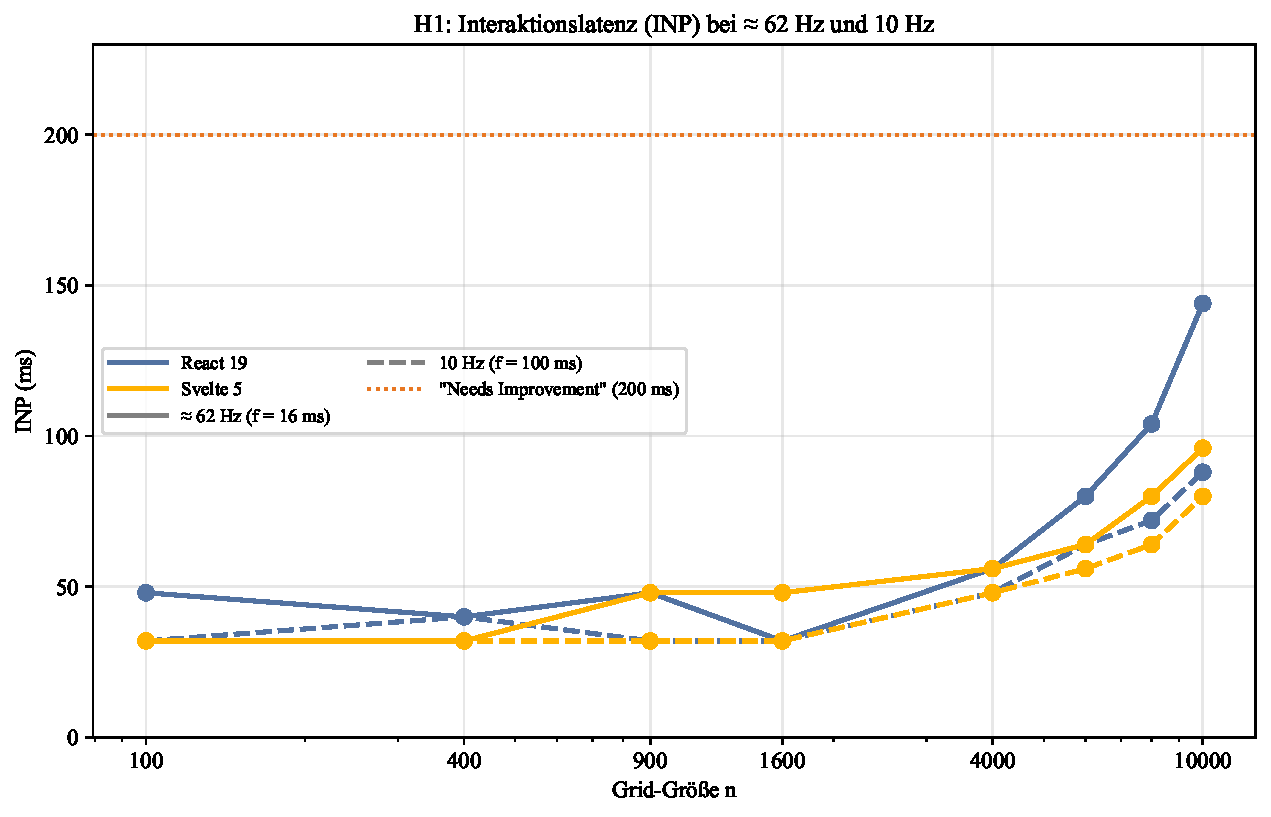
\includegraphics[width=\textwidth,keepaspectratio]{bilder/h1_inp}
  \caption[H1 – INP beider Frameworks bei $f \approx 62\,\text{Hz}$ und $f = 10\,\text{Hz}$ über alle $n$-Stufen]{H1 – INP beider Frameworks bei $f \approx 62\,\text{Hz}$ und $f = 10\,\text{Hz}$
           über alle $n$-Stufen (\cref{ss:inp}).}
  \label{fig:h1-inp}
\end{figure}

\subsection{Zerlegung der INP-Phasen}
\label{ss:results-h1-phases}

\Cref{tab:inp-phases} teilt die INP-Komponenten \textit{inputDelay} (iD), \textit{processingTime} (pT) und \textit{presentationDelay} (pD) für ausgewählte Szenarien auf und zeigt, in welcher Phase die Latenz entsteht (\cref{ss:inp}). Die \textit{processingTime} trägt in keinem Szenario wesentlich zum INP bei: Sie überschreitet $1{,}0\,\text{ms}$ bei React nicht (Maximum: $n = 4000$, $f = 20\,\text{Hz}$) und beträgt für Svelte selbst unter Extremlast ($n = 10\,000$, $f \approx 62\,\text{Hz}$) lediglich $0{,}7\,\text{ms}$. Die INP-Verschlechterung mit steigendem~$n$ wird damit ausschließlich durch \textit{inputDelay} (blockierter Main Thread) und \textit{presentationDelay} (Rendering nach dem Handler) bestimmt. Wie sich die Latenz auf diese beiden Phasen verteilt, hängt von der Last ab (\cref{tab:inp-phases}). Bei niedriger Last ($n \leq 1600$) macht die \textit{presentationDelay} den größten Anteil aus: Bei React, $n = 100$, $f = 10\,\text{Hz}$ beträgt der \textit{inputDelay} lediglich $0{,}4\,\text{ms}$, während die \textit{presentationDelay} $31{,}5\,\text{ms}$ ausmacht. Bei hoher UI-Dichte und niedriger Frequenz ($n = 10\,000$, $f = 10\,\text{Hz}$) bleibt die \textit{presentationDelay} zwar der größte Anteil ($51{,}9\,\text{ms}$), der \textit{inputDelay} wächst jedoch auf $36{,}1\,\text{ms}$ an und trägt damit spürbar zum INP bei. Unter Extremlast kann der \textit{inputDelay} die \textit{presentationDelay} schließlich überschreiten: Bei React, $n = 8000$, $f \approx 62\,\text{Hz}$ beträgt er $69{,}6\,\text{ms}$ gegenüber $34{,}4\,\text{ms}$. In nahezu allen Szenarien überwiegt die \textit{presentationDelay} weiterhin; die beschriebene Ausnahme bleibt auf dieses eine Szenario beschränkt. Hauptursache des wachsenden \textit{inputDelay} sind die in \cref{s:results-h2} gemessenen Scripting-Kosten, die den Main Thread blockieren. Szenariospezifische Besonderheiten werden nachfolgend diskutiert. Eine Ausnahme zeigt jedoch, dass ein niedrigerer Scripting-Aufwand nicht automatisch zu einem besseren INP führt (\cref{tab:inp-phases}, unterer Abschnitt). 

\noindent\textbf{Ausnahme\,1} ($n = 10\,000$, $f = 20\,\text{Hz}$): React erzielt einen INP von $96\,\text{ms}$ (iD: $20{,}9\,\text{ms}$; pT: $0\,\text{ms}$; pD: $75{,}1\,\text{ms}$), Svelte einen INP von $104\,\text{ms}$ (iD: $18{,}0\,\text{ms}$; pT: $0\,\text{ms}$; pD: $86{,}0\,\text{ms}$). Svelte weist sowohl geringere Scripting-Kosten als auch einen niedrigeren \textit{inputDelay} auf und erzielt dennoch den höheren INP. Die Ursache liegt in der \textit{presentationDelay} ($86{,}0\,\text{ms}$ vs. $75{,}1\,\text{ms}$). Sveltes höhere Rendering-Zeit bei $f = 20\,\text{Hz}$ ($13{,}71\,\text{ms}$ vs. $11{,}87\,\text{ms}$, vgl. \cref{ss:results-h2-scripting}) spricht für dieselbe Ursache, erklärt quantitativ jedoch nur einen Teil des \textit{presentationDelay}-Unterschieds von $10{,}9\,\text{ms}$. Der genaue Mechanismus der verbleibenden Differenz lässt sich anhand der vorliegenden Daten nicht bestimmen. Das zeigt: Geringere Scripting-Kosten garantieren keinen besseren INP; der Rendering-Nachteil kann den Scripting-Vorteil überwiegen. Daneben bestätigt die Phasenzerlegung einen zweiten Aspekt von H1 unmittelbar (\cref{tab:inp-phases}). 

\noindent\textbf{H1-Bestätigung} ($n = 1600$, $f \geq 30\,\text{Hz}$): Bei $\Delta t = 16\,\text{ms}$ beträgt der INP für React $32\,\text{ms}$ (iD: $5{,}5\,\text{ms}$; pT: $0{,}1\,\text{ms}$; pD: $26{,}4\,\text{ms}$), für Svelte hingegen $48\,\text{ms}$ (iD: $4{,}6\,\text{ms}$; pT: $0\,\text{ms}$; pD: $43{,}4\,\text{ms}$). Bei $\Delta t = 33\,\text{ms}$ gilt dasselbe: React $32\,\text{ms}$ (iD: $6{,}7\,\text{ms}$; pT: $0{,}2\,\text{ms}$; pD: $25{,}1\,\text{ms}$) gegenüber Svelte $40\,\text{ms}$ (iD: $4{,}5\,\text{ms}$; pT: $0\,\text{ms}$; pD: $35{,}5\,\text{ms}$). In diesen Szenarien liegen die Scripting- und Rendering-Kosten beider Frameworks auf einem niedrigen Wert (Scripting: $0{,}75$--$1{,}61\,\text{ms}$/Tick; Rendering: $1{,}73$--$1{,}91\,\text{ms}$/Tick); die Rendering-Zeiten sind dabei nahezu gleich ($f \approx 62\,\text{Hz}$: $1{,}75$ vs. $1{,}73\,\text{ms}$/Tick; $f \approx 30\,\text{Hz}$: $1{,}91$ vs. $1{,}87\,\text{ms}$/Tick). Svelte weist bei beiden Frequenzstufen den niedrigeren \textit{inputDelay} auf ($4{,}6\,\text{ms}$ bzw.\ $4{,}5\,\text{ms}$ gegenüber $5{,}5\,\text{ms}$ bzw.\ $6{,}7\,\text{ms}$ bei React). Dennoch überwiegt der Unterschied in der \textit{presentationDelay} im Gesamtergebnis: Er beträgt $17{,}0\,\text{ms}$ ($f \approx 62\,\text{Hz}$) bzw.\ $10{,}4\,\text{ms}$ ($f \approx 30\,\text{Hz}$) zugunsten Reacts und bestimmt damit den höheren INP von Svelte. Die Ursache dieses pD-Unterschieds unterscheidet sich von Ausnahme\,1: Dort lag sie in Sveltes höherer Rendering-Zeit. Hier sind die Rendering-Zeiten nahezu identisch, sodass ein Scheduling-Effekt als Erklärung naheliegt. Als mögliche Ursache kommt Reacts prioritätsbasiertes Scheduling infrage, das Klick-Events gegenüber Hintergrund-Updates priorisiert, während Sveltes synchrones Effect-Batching vergleichbare Priorisierungsmöglichkeiten nicht vorsieht (\cref{sss:scheduling-priotising-of-updates,sss:microtasks}); der genaue Mechanismus lässt sich anhand der vorliegenden Daten nicht bestimmen. Dieser Scheduling-Vorteil Reacts tritt ausschließlich ab $f \geq 30\,\text{Hz}$ auf; bei $n = 1600$ und $f = 10\,\text{Hz}$ sowie $f = 20\,\text{Hz}$ sind die INP-Werte beider Frameworks gleich ($32\,\text{ms}$, vgl.~\cref{tab:appendix-benchmark}). Dieses Ergebnis ist konsistent mit H1: Bei Last unterhalb des Frame-Budgets stabilisiert Reacts Scheduling den INP, auch wenn die absoluten Scripting-Kosten höher sind — bei $n = 1600$ und $f \approx 62\,\text{Hz}$ beträgt der INP-Vorteil $16\,\text{ms}$ (React $32\,\text{ms}$ vs.\ Svelte $48\,\text{ms}$, $+50\,\%$) — ein Scheduling-Vorteil, kein Effizienz-Vorteil.

\noindent\textbf{Ausnahme\,2} ($n = 10\,000$, $f \approx 30\,\text{Hz}$, \cref{tab:inp-phases}) bildet eine weitere, durch H1 nicht abgedeckte Einschränkung: Beide Frameworks erzielen denselben INP ($104\,\text{ms}$), jedoch mit gegenläufiger Phasenverteilung. React weist einen \textit{inputDelay} von $5\,\text{ms}$ auf, was mit dem in der H1-Bestätigung beschriebenen Scheduling-Vorteil konsistent ist (\cref{sss:scheduling-priotising-of-updates}), während Sveltes \textit{inputDelay} $51{,}8\,\text{ms}$ beträgt (der höchste Svelte-Wert im gesamten Datensatz). Eine \textit{presentationDelay} von $99\,\text{ms}$ hebt diesen Vorteil jedoch vollständig auf. Bei einer Rendering-Zeit von $8{,}40\,\text{ms}$/Tick entspricht dies der höchsten React-\textit{presentationDelay} im Datensatz, deren Ursache sich mit den erhobenen Metriken nicht eindeutig bestimmen lässt (vgl.~\cref{s:limitations}). Der Gleichstand ergibt sich damit als Überlagerung des Scheduling-Vorteils Reacts mit einem ungeklärten \textit{presentationDelay}-Ausreißer; kein Widerspruch zu H1, aber eine weitere Einschränkung.
\begin{table}[H]
  \centering
  \caption[INP-Phasenzerlegung für ausgewählte Szenarien]{INP-Phasenzerlegung für ausgewählte Szenarien (Datenquelle:
           \texttt{summary.csv}, vgl.~\cref{ss:impl-results})}
  \label{tab:inp-phases}
  \small
  \begin{tabular}{llrrrrr}
    \toprule
    \textbf{Framework} & \textbf{Szenario}
      & \textbf{INP} & \textbf{iD} & \textbf{pT} & \textbf{pD}
      & \textbf{Scripting} \\
    & ($n$\,/\,$f$)
      & (ms) & (ms) & (ms) & (ms)
      & (ms/Tick) \\
    \midrule
    \multicolumn{7}{l}{\textit{Niedrige Last (pD-bestimmt)}} \\
    React  & 100\,/\,$10\,\text{Hz}$
      & 32  & 0{,}4  & 0{,}1 & 31{,}5 & 0{,}27 \\
    \midrule
    \multicolumn{7}{l}{\textit{Hohe Last (iD wächst)}} \\
    React  & 10\,000\,/\,$10\,\text{Hz}$
      & 88  & 36{,}1 & 0{,}0 & 51{,}9 & 11{,}24 \\
    Svelte & 10\,000\,/\,$10\,\text{Hz}$
      & 80  & 1{,}9  & 0{,}0 & 78{,}1 & 4{,}12 \\
    \midrule
    \multicolumn{7}{l}{\textit{Extremlast (iD $>$ pD)}} \\
    React  & 8\,000\,/\,${\approx}\,62\,\text{Hz}$
      & 104 & 69{,}6 & 0{,}0 & 34{,}4 & 3{,}53 \\
    Svelte & 8\,000\,/\,${\approx}\,62\,\text{Hz}$
      & 80  & 32{,}1 & 0{,}0 & 47{,}9 & 3{,}08 \\
    \midrule
    \multicolumn{7}{l}{\textit{Ausnahme\,1: Svelte-INP $>$ React trotz niedrigerem iD}} \\
    React  & 10\,000\,/\,$20\,\text{Hz}$
      & 96  & 20{,}9 & 0{,}0 & 75{,}1 & 11{,}17 \\
    Svelte & 10\,000\,/\,$20\,\text{Hz}$
      & 104 & 18{,}0 & 0{,}0 & 86{,}0 & 4{,}29 \\
    \midrule
    \multicolumn{7}{l}{\textit{H1-Bestätigung: Scheduling-Vorteil React bei $n = 1600$, $f \geq 30\,\text{Hz}$}} \\
    React  & 1\,600\,/\,${\approx}\,62\,\text{Hz}$
      & 32  & 5{,}5  & 0{,}1 & 26{,}4 & 1{,}57 \\
    Svelte & 1\,600\,/\,${\approx}\,62\,\text{Hz}$
      & 48  & 4{,}6  & 0{,}0 & 43{,}4 & 0{,}75 \\
    React  & 1\,600\,/\,${\approx}\,30\,\text{Hz}$
      & 32  & 6{,}7  & 0{,}2 & 25{,}1 & 1{,}61 \\
    Svelte & 1\,600\,/\,${\approx}\,30\,\text{Hz}$
      & 40  & 4{,}5  & 0{,}0 & 35{,}5 & 0{,}76 \\
    \midrule
    \multicolumn{7}{l}{\textit{Ausnahme\,2: Gleichstand trotz gegenläufiger Phasenverteilung}} \\
    React  & 10\,000\,/\,${\approx}\,30\,\text{Hz}$
      & 104 & 5{,}0  & 0{,}0 & 99{,}0 & 7{,}43 \\
    Svelte & 10\,000\,/\,${\approx}\,30\,\text{Hz}$
      & 104 & 51{,}8 & 0{,}0 & 52{,}2 & 4{,}09 \\
    \bottomrule
  \end{tabular}
\end{table}

\subsection{Bewertung von H1}
\label{ss:results-h1-verdict}

Über alle vier Frequenzstufen hinweg weist Svelte bei hoher UI-Dichte ($n \geq 4000$) in zwölf von 16~Szenarien einen niedrigeren INP auf als React. In zwei weiteren Szenarien ($n = 4000$, $f = 10\,\text{Hz}$ und $f \approx 62\,\text{Hz}$) sind die INP-Werte beider Frameworks gleich ($48\,\text{ms}$ bzw.\ $56\,\text{ms}$). Der in H1 erwartete Svelte-Vorteil bei hoher Dichte (\cref{ss:hypotheses}) zeigt sich durch die höheren Scripting-Kosten von React (\cref{s:results-h2}), die primär den \textit{inputDelay} erhöhen ($n = 10\,000$, $f = 10\,\text{Hz}$: $36{,}1\,\text{ms}$ gegenüber $1{,}9\,\text{ms}$ bei Svelte). Anzumerken ist, dass bei $n = 10\,000$ und $f \approx 62\,\text{Hz}$ (dem Szenario mit dem größten INP-Abstand, $96\,\text{ms}$ vs.\ $144\,\text{ms}$) Svelte trotz geringfügig höherer Scripting-Zeit ($3{,}66\,\text{ms}$ vs.\ $3{,}42\,\text{ms}$, vgl.~\cref{ss:results-h2-scripting}) einen niedrigeren \textit{inputDelay} aufweist ($34{,}1\,\text{ms}$ vs.\ $56{,}9\,\text{ms}$). Der direkte Kausalzusammenhang Scripting\,$\rightarrow$\,\textit{inputDelay} greift bei $f \approx 62\,\text{Hz}$ somit nicht; dies deutet auf frequenzabhängige Scheduling-Effekte hin. Bei niedriger Dichte weist Svelte ebenfalls niedrigere INP-Werte auf: bei $n = 100$ ausschließlich bei $f \approx 62\,\text{Hz}$ ($32\,\text{ms}$ vs.\ $48\,\text{ms}$), bei $n = 400$ sowohl bei $f \approx 62\,\text{Hz}$ als auch bei $f = 10\,\text{Hz}$ (jeweils $32\,\text{ms}$ vs.\ $40\,\text{ms}$). In allen diesen Fällen resultiert der Unterschied ausschließlich aus der \textit{presentationDelay}, da die Scripting-Kosten auf diesen Stufen vernachlässigbar sind. Der in H1 ebenfalls vorhergesagte Scheduling-Vorteil Reacts bei Last unterhalb des Frame-Budgets bestätigt sich bei $n = 1600$ und $f \geq 30\,\text{Hz}$ (vgl.~\cref{ss:results-h1-phases}). Zwei Szenarien, in denen die \textit{presentationDelay} das durch H1 vorhergesagte INP-Ergebnis überlagert, schränken die Gesamtaussage ein: Bei $n = 10\,000$ und $f = 20\,\text{Hz}$ übersteigt Sveltes INP den von React infolge einer höheren \textit{presentationDelay} durch Rendering-Bündelung (\cref{ss:results-h1-phases}). Bei $n = 10\,000$ und $f \approx 30\,\text{Hz}$ ergibt sich ein Gleichstand mit gegenläufiger, ungeklärter Phasenverteilung (\cref{ss:results-h1-phases}). Da der Svelte-Vorteil in der deutlichen Mehrheit der Szenarien bei $n \geq 4000$ gilt und beide Teilaussagen von H1 empirisch bestätigt sind, stützen die Befunde H1 trotz dieser Einschränkungen. \textbf{H1 wird bestätigt.}

\section{H4: Identifikation des Tipping Points}
\label{s:results-h4}

Während H2 beschreibt, wie stark der Scripting-Aufwand mit $n$ wächst, fragt H4, ab welchem $n$ das Frame-Budget überschritten wird und welches Framework diesen Tipping Point zuerst erreicht (\cref{ss:hypotheses}).

\subsection{Frame-Budget-Auslastung und Long Tasks}
\label{ss:results-h4-tipping}

\Cref{fig:h4-tipping}a zeigt, bei welchem $n$ die kombinierte Summe aus Scripting- und Rendering-Zeit die $16{,}7\,\text{ms}$-Grenze des Frame-Budgets bei $f = 20\,\text{Hz}$ überschreitet. React erreicht diesen Schwellenwert bei einer niedrigeren UI-Dichte als Svelte. Dies bestätigt die Vorhersage aus \cref{sss:tipping-point}: Die Abstraktionskosten der Fiber-Architektur führen dazu, dass der Main Thread bei React früher vollständig ausgelastet ist als bei Svelte mit seiner feingranularen Reaktivität.
Zu beachten ist, dass die $16{,}7\,\text{ms}$-Grenze als Frame-Budget nur dann direkt relevant ist, wenn Tick-Intervall und Framelänge übereinstimmen ($f \approx 62\,\text{Hz}$). Bei niedrigeren Frequenzen bedeutet eine Überschreitung dieser Grenze nicht zwingend einen Frame-Drop, da der Main Thread zwischen den Ticks ausreichend Zeit für das Rendering hat (\cref{sss:frame-budget}). Die Anzahl der Long Tasks (\cref{fig:h4-tipping}b) bestätigt dies bei niedrigen bis mittleren Frequenzen, zeigt jedoch bei $f \approx 62\,\text{Hz}$ eine Umkehr des Long-Task-Verhältnisses. Bei $f \approx 30\,\text{Hz}$ und $n = 10\,000$ erzeugt React rund $45$ Long Tasks, Svelte $22{,}5$. Die IQR-Streuung ist dabei hoch (React: $27$, Svelte: $28$; aus Rohdaten, nicht in \cref{tab:appendix-benchmark}); bei Svelte übersteigt der IQR sogar den Median, was die Aussagekraft dieses Vergleichs einschränkt. Ab $f \approx 62\,\text{Hz}$ dreht sich das Verhältnis: Svelte erzeugt $91$ Long Tasks gegenüber $86$ bei React. Diese Umkehrung tritt ausschließlich bei $n = 10\,000$ auf; bei $n = 8000$ und $f \approx 62\,\text{Hz}$ hat React mit $58$ Long Tasks weiterhin deutlich mehr als Svelte mit $29$. Es handelt sich somit nicht um ein generelles Muster, sondern um einen Extremlast-Effekt: Bei $f \approx 62\,\text{Hz}$ stapelt Sveltes synchrones Effect-Batching (\cref{sss:microtasks,sss:scheduling-priotising-of-updates}) Arbeit ohne zwischenzeitliches Yielding, was zu einem überproportionalen Anstieg der Long Tasks führt (Svelte: $+\!304\,\%$; React: $+\!91\,\%$). Der Scripting-Schnittpunkt (\cref{ss:results-h2-scripting}) tritt im selben Szenario auf und ist konsistent mit diesem Befund.
\begin{figure}[H]
  \centering
  \begin{minipage}[t]{\textwidth}
    \centering
    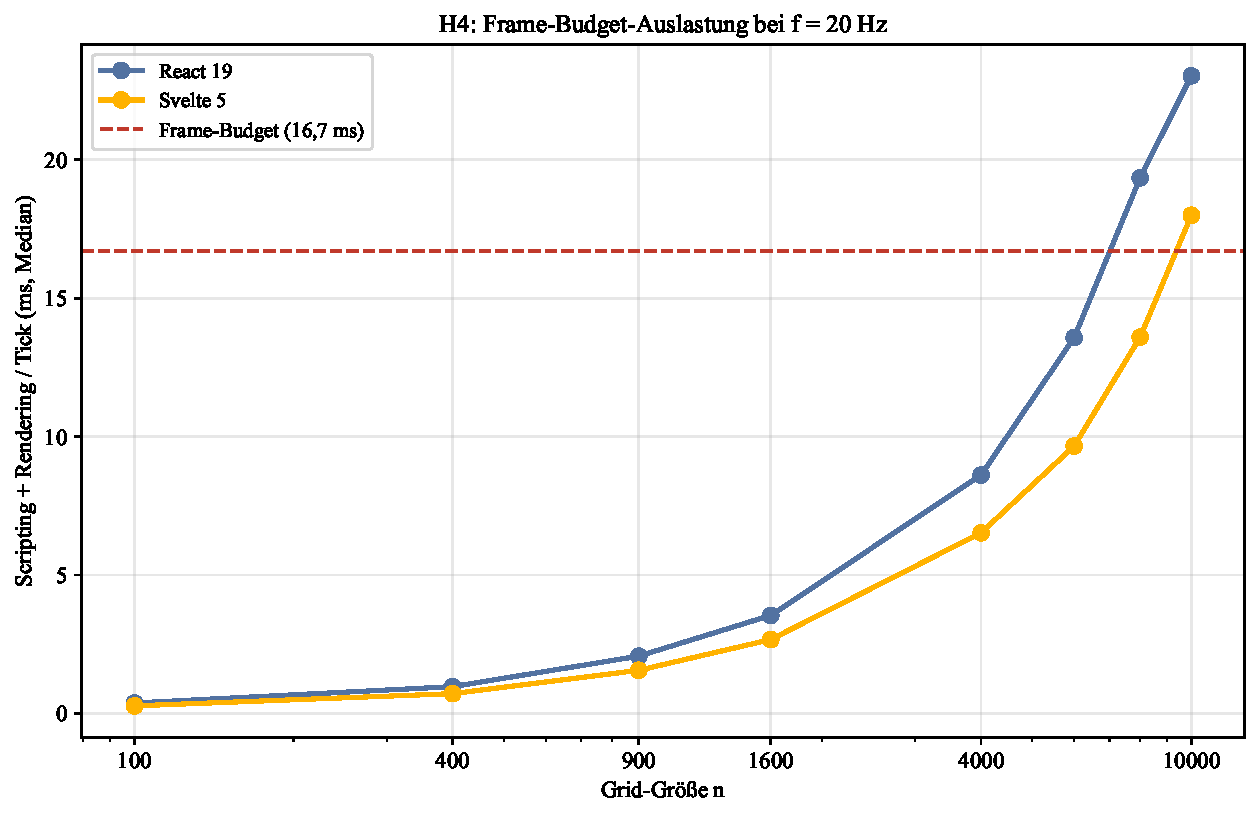
\includegraphics[width=\textwidth,keepaspectratio]{bilder/h4_frame_budget}
    \subcaption{(Scripting + Rendering) vs. $16{,}7\,\text{ms}$-Grenze bei $f = 20\,\text{Hz}$}
    \label{fig:h4-budget}
  \end{minipage}
  \vspace{0.75em}
  \begin{minipage}[t]{\textwidth}
    \centering
    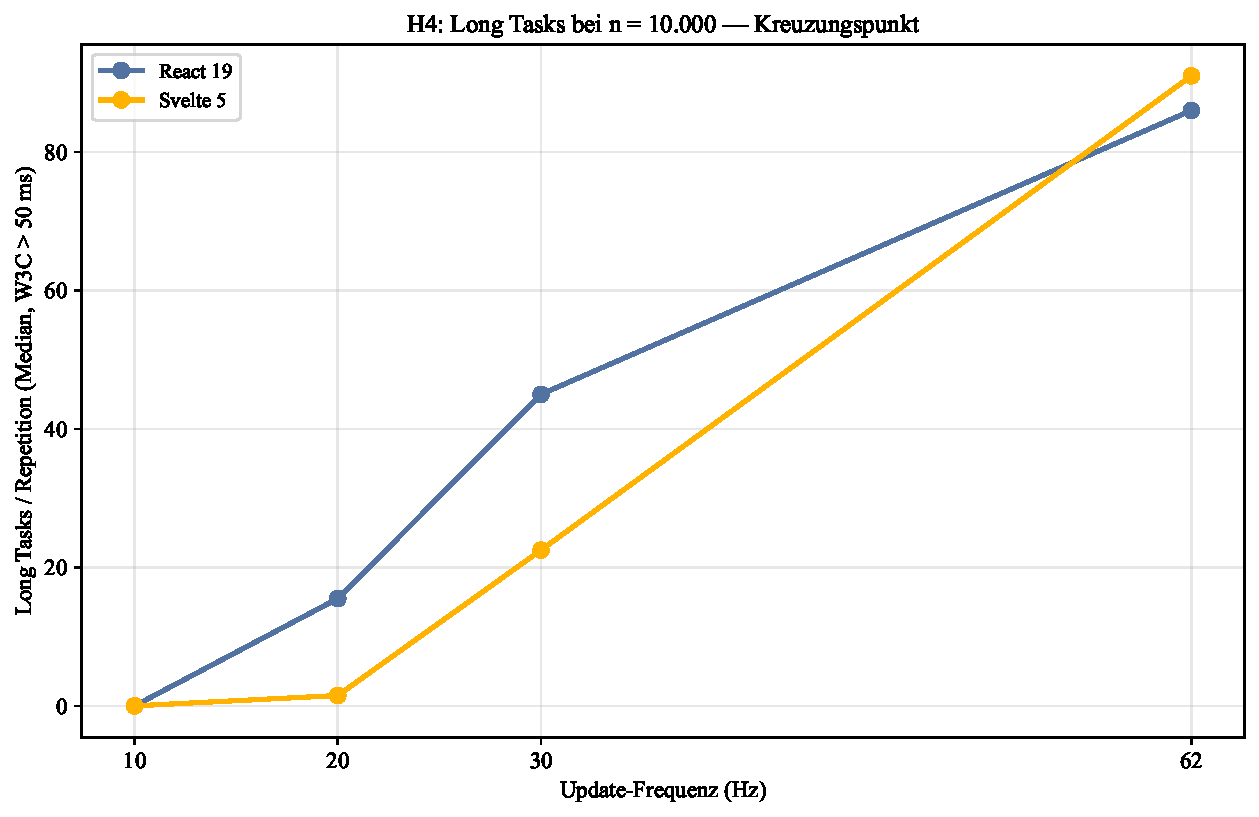
\includegraphics[width=\textwidth,keepaspectratio]{bilder/h4_long_tasks}
    \subcaption{Long Tasks bei $n = 10\,000$ über alle Frequenzstufen}
    \label{fig:h4-longtasks}
  \end{minipage}
  \caption[H4 – Tipping-Point-Analyse: Frame-Budget-Auslastung und Long Tasks]{H4 – Tipping-Point-Analyse: (a) Frame-Budget-Auslastung beider Frameworks
           bei $f = 20\,\text{Hz}$ mit $16{,}7\,\text{ms}$-Grenze; (b) Anzahl der Long Tasks bei $n = 10\,000$
           in Abhängigkeit von $f$
           (vgl.~\cref{sss:frame-budget,sss:long-task-measurement}).}
  \label{fig:h4-tipping}
\end{figure}

\subsection{Bewertung von H4}
\label{ss:results-h4-verdict}

Die Frame-Budget-Auswertung bestätigt die Hauptvorhersage von H4: React überschreitet die $16{,}7\,\text{ms}$-Grenze bei niedrigerer UI-Dichte als Svelte (\cref{sss:tipping-point}). Bei $f = 10\,\text{Hz}$ überschreitet React die Grenze ab $n = 8000$ ($19{,}59\,\text{ms}$), Svelte erst ab $n = 10\,000$ ($17{,}67\,\text{ms}$); bei $f = 20\,\text{Hz}$ zeigt sich dasselbe Muster: React ab $n = 8000$ ($19{,}35\,\text{ms}$), Svelte ab $n = 10\,000$ ($18{,}00\,\text{ms}$). Diese Grenzüberschreitung pro Tick tritt ausschließlich bei $f \leq 20\,\text{Hz}$ auf. Die konkret ermittelten $n$-Schwellenwerte sind V8\slash Chromium-spezifisch; andere JavaScript-Engines könnten den Tipping Point bei abweichenden $n$-/$f$-Kombinationen aufweisen (vgl.~\cref{s:limitations}). Bei $f \approx 30\,\text{Hz}$ erreicht die kombinierte Scripting- und Rendering-Zeit für React maximal $15{,}83\,\text{ms}$ ($n = 10\,000$: $7{,}43 + 8{,}40\,\text{ms}$), bei $f \approx 62\,\text{Hz}$ lediglich $8{,}37\,\text{ms}$ ($3{,}42 + 4{,}95\,\text{ms}$), jeweils unterhalb der Schwelle (vgl.~\cref{tab:appendix-benchmark}). Die Long-Task-Analyse zeigt bei $n = 10\,000$ und $f \approx 62\,\text{Hz}$ eine Umkehr des Long-Task-Verhältnisses (Svelte $91$ vs. React $86$ Long Tasks). Diese Umkehr belegt empirisch die in H4 vorhergesagte mögliche Rangfolge-Umkehr bei extremer Last (\cref{sss:tipping-point}). \textbf{H4 wird bestätigt.}

\section{Zusammenfassung der Ergebnisse}
\label{s:results-summary}

\Cref{tab:hypotheses-summary} fasst die Bewertungen der vier Hypothesen zusammen. H2 und H3 erklären die Befunde von H1 und H4: Die in H2 gemessenen Scripting-Kosten der Fiber-Architektur (\cref{s:results-h2}) begründen, warum React in H1 früher INP-Verschlechterungen zeigt (\cref{s:results-h1}) und in H4 das Frame-Budget bei niedrigerer UI-Dichte überschreitet (\cref{s:results-h4}). Die in H3 gemessenen Heap-Delta-Unterschiede (\cref{s:results-h3}) belegen, dass die zusätzlichen Abstraktionskosten nicht nur die CPU, sondern auch den Speicher belasten. H4 baut auf den CPU-Kurven aus H2 auf, wertet diese schwellenwertbasiert aus und bestimmt damit den Übergang vom kontrollierten Skalierungsbereich zur Main-Thread-Blockierung.
\begin{table}[H]
  \centering
  \caption{Zusammenfassung der Hypothesenbewertungen (H1–H4)}
  \label{tab:hypotheses-summary}
  \small
  \begin{tabular}{llp{7.5cm}}
    \toprule
    \textbf{Hypothese} & \textbf{Ergebnis} & \textbf{Kernaussage} \\
    \midrule
    H1 & bestätigt &
      Svelte erzielt bei $n \geq 4000$ in der Mehrzahl der Szenarien niedrigere
      INP-Werte; Reacts Scheduling-Vorteil zeigt sich erwartungsgemäß bei
      $n = 1600\,/\,{\geq}30\,\text{Hz}$; ungeklärte Ausnahmen bei
      $n = 10\,000\,/\,20\,\text{Hz}$ (Svelte schlechter) und
      $n = 10\,000\,/\,30\,\text{Hz}$ (Gleichstand). \\[4pt]
    H2 & teilweise bestätigt &
      Reacts Scripting-Aufwand pro Tick wächst bei $f \leq 30\,\text{Hz}$ stärker
      als Sveltes; bei $f \approx 62\,\text{Hz}$ und $n = 10\,000$ tritt
      ein Scripting-Schnittpunkt auf (Svelte $3{,}66\,\text{ms}$ vs. React $3{,}42\,\text{ms}$). \\[4pt]
    H3 & bestätigt &
      Qualitativ bestätigt durch Retained Size: React $131\,\text{kB}$
      vs.\ Svelte $19{,}8\,\text{kB}$ (${\approx}1310$ vs.\ ${\approx}198$\,B
      pro Komponente) bei $n = 100$ im Dev-Build
      (vgl.~\cref{tab:heap-qualitative}); quantitativ im Production-Build:
      Heap-Delta-Faktor $2{,}8\times$ ($n = 100$) bis $6{,}4\times$
      ($n = 6000$), danach leicht rückläufig. \\[4pt]
    H4 & bestätigt &
      React überschreitet das $16{,}7\,\text{ms}$-Frame-Budget bei
      niedrigerem $n$ als Svelte; bei $n = 10\,000\,/\,62\,\text{Hz}$
      erzeugt Svelte mehr Long Tasks ($91$ vs.~$86$). \\
    \bottomrule
  \end{tabular}
\end{table}

\section{Limitationen}
\label{s:limitations}

Die folgenden Einschränkungen betreffen die Interpretierbarkeit der konkreten Befunde und ergänzen die in \cref{ss:external-validity} diskutierte externe Validität des Versuchsdesigns.

\subsection{Fehlende Isolation des Compiler-Einflusses}
React~19 wurde ausschließlich mit aktiviertem Compiler gemessen. Der Compiler lässt das komponentenbasierte Render-Modell und die Fiber-Architektur unverändert; die Reconciliation wird weiterhin ausgeführt (\cref{sss:potentials-and-limitations}). Daher lässt sich im gewählten Versuchsaufbau nicht bestimmen, welcher Anteil der gemessenen Scripting-Kosten auf die Compiler-Memoisierung und welcher auf die VDOM-Reconciliation entfällt. Ein Test ohne Compiler hätte diesen Einfluss isolierbar gemacht, hätte jedoch die praktische Vergleichbarkeit beeinträchtigt, da Sveltes Vorteile ebenfalls durch Compile-Time-Optimierung entstehen (\cref{ss:svelte-compiler}).

\subsection{Ausschließlich Chromium}
Alle Messungen basieren auf Playwrights Chromium-Instanz mit V8 als JavaScript-Engine. Da die Messergebnisse das JIT-Verhalten von V8 widerspiegeln (\cref{sss:jit-interference}), könnten andere Engines — SpiderMonkey (Firefox) und JavaScriptCore (Safari) — den Tipping Point bei anderen $n$-/$f$-Kombinationen aufweisen. Die Ergebnisse gelten daher primär für Chromium-basierte Umgebungen.

\subsection{Verbleibende Browser-interne Störeinflüsse}
Trotz der in \cref{sss:gc-interference,sss:jit-interference} beschriebenen Vorkehrungen lassen sich Garbage-Collection-Pausen und JIT-Effekte nicht vollständig ausschließen. Der ungleichmäßige Scripting-Rückgang bei höherer Tick-Frequenz (\cref{ss:results-h2-scripting}) ist ohne V8-internes Profiling nicht eindeutig erklärbar und wurde daher im vorliegenden Kapitel als Spekulation gekennzeichnet.

\subsection{Presentationdelay als zusammengesetzte Metrik}
Die \textit{presentationDelay} erfasst die Zeit nach Abschluss der Skriptausführung bis zur sichtbaren Darstellung der Änderungen als einzelne Kennzahl (\cref{ss:inp}). Eine Zerlegung in Browser-interne Teilphasen (Layout, Paint, Composite) war nicht Teil der erhobenen Metriken. Bei $n = 10\,000$ und $f = 10\,\text{Hz}$ weist Svelte eine deutlich höhere \textit{presentationDelay} auf als React ($78{,}1\,\text{ms}$ vs.\ $51{,}9\,\text{ms}$, vgl.~\cref{tab:inp-phases}), obwohl die Rendering-Zeiten pro Tick nahezu identisch sind ($13{,}55\,\text{ms}$ vs.\ $13{,}31\,\text{ms}$, vgl.~\cref{ss:results-h2-scripting}). Die Ursache dieser Diskrepanz lässt sich mit den erhobenen Metriken nicht eindeutig bestimmen. Anzumerken ist, dass das Phänomen nicht auf ein Framework beschränkt ist. Bei $n = 10\,000$ und $f \approx 30\,\text{Hz}$ weist umgekehrt React die höchste \textit{presentationDelay} im gesamten Datensatz auf ($99\,\text{ms}$ bei $8{,}40\,\text{ms}$/Tick Rendering-Zeit), während Sveltes \textit{presentationDelay} dort $52{,}2\,\text{ms}$ beträgt, auch hier ohne eindeutig bestimmbare Ursache. Dies stellt eine Grenze der Interpretierbarkeit der INP-Phasenzerlegung dar.

\chapter{Fazit}
\label{ch:fazit}

\section{Beantwortung der Forschungsfrage}
\label{s:fazit-forschungsfrage}

Die empirischen Ergebnisse zeigen, dass der Leistungsunterschied zwischen React~19 und Svelte~5 unter kombinierter Dauerlast nicht rein quantitativ, sondern architektonisch bedingt ist. Entscheidend ist dabei, dass dieselbe Architektureigenschaft jeweils Vor- und Nachteil zugleich erzeugt: Der Reconciliation-Overhead der Fiber-Engine, der bei hoher UI-Dichte zu erhöhten Scripting-Kosten, höherem Speicherbedarf und einem früheren Tipping Point führt, ermöglicht bei moderater Last und hoher Update-Frequenz ein Scheduling-Modell, das den INP stabilisiert. Umgekehrt schließt Sveltes feingranulare Reaktivität, die den Effizienzvorteil bei hoher Dichte begründet, ein vergleichbares Priorisierungsmodell aus und führt unter Extremlast zu einer Umkehr der Long-Task-Rangfolge. Eine vollständige Übersicht der Messbefunde und Hypothesenbewertungen findet sich in \cref{tab:hypotheses-summary}. Kein Framework ist damit uneingeschränkt überlegen; welches besser skaliert, lässt sich nur lastabhängig beantworten. Die vorliegende Untersuchung schließt damit die in \cref{s:ausgangssituation,s:research-gap} identifizierten Lücken der bisherigen Forschung: Nach aktuellem Stand der Literatur lagen bislang weder vergleichbare empirische Messdaten für React~19 mit aktiviertem Compiler und Svelte~5 mit Runes unter kombinierter Dauerlast vor, noch wurden INP und Frame-Budget-Überschreitung als Metriken für diese Frameworks systematisch erfasst und ausgewertet.

\section{Handlungsempfehlung für die Praxis}
\label{s:fazit-empfehlung}

Für datenintensive Echtzeit-Anwendungen wie Monitoring-Dashboards (\cref{s:motivation}) lassen sich auf Basis der empirischen Ergebnisse vier Szenarien unterscheiden:

\noindent Für Anwendungen mit \textbf{hoher UI-Dichte} bietet Svelte~5 strukturelle Vorteile: Der geringere Scripting-Aufwand verschiebt den Tipping Point zu höheren $n$-Werten (\cref{s:results-h2,s:results-h4}); in der Mehrzahl der gemessenen Szenarien erzielt Svelte zudem niedrigere INP-Werte (\cref{ss:results-h1-verdict}). Zwei Ausnahmen schränken diesen Vorteil bei maximaler UI-Dichte ein (\cref{ss:results-h1-phases}).

\noindent In \textbf{speicherkritischen Umgebungen}, etwa auf ressourcenbeschränkten Endgeräten oder bei Anwendungen mit vielen gleichzeitig aktiven Komponenteninstanzen, ist Svelte~5 ebenfalls klar im Vorteil, da der Heap-Verbrauch (wie die internen Datenstrukturen beider Frameworks belegen) strukturell niedriger ausfällt (\cref{s:results-h3}).

\noindent Bei \textbf{moderater UI-Dichte und hoher Update-Frequenz} kann React~19 die bessere Wahl sein: Das prioritätsbasierte Scheduling der Fiber-Engine erzielt in diesem Lastbereich niedrigere INP-Werte (\cref{ss:results-h1-phases}). Dieser Vorteil tritt ausschließlich unterhalb des Tipping Points auf, ab dem Reacts höhere Scripting-Kosten das Frame-Budget überschreiten (\cref{ss:results-h4-tipping}); bei steigender UI-Dichte überwiegen die strukturellen Vorteile von Svelte.

\noindent Bei \textbf{niedriger UI-Dichte} sind die gemessenen Unterschiede insgesamt gering; Svelte~5 zeigt vereinzelt leichte INP-Vorteile (\cref{ss:results-h1-verdict}). Die Framework-Entscheidung kann in diesem Fall anhand anderer Kriterien wie Ökosystem, Entwicklererfahrung oder bestehender Codebasis getroffen werden.

\noindent In allen Szenarien gilt: Die hier ermittelten konkreten Last-Schwellenwerte sind V8- und Chromium-spezifisch; andere JavaScript-Engines können ein abweichendes Skalierungsverhalten zeigen (\cref{s:limitations}).

\section{Ausblick}
\label{s:fazit-ausblick}

Aus den Ergebnissen dieser Arbeit ergeben sich vier Richtungen für weiterführende Forschung.

\noindent\textbf{Übertragbarkeit auf andere JavaScript-Engines.} Die ermittelten Schwellenwerte und der Scripting-Schnittpunkt bei $f \approx 62\,\text{Hz}$ beruhen auf V8s JIT-Optimierungsprofil (\cref{s:limitations}). Eine vergleichende Studie unter SpiderMonkey und JavaScriptCore würde klären, ob die architektonischen Unterschiede zwischen signalbasierter Reaktivität und VDOM-Reconciliation engine-unabhängige Skalierungseigenschaften erzeugen oder ob die beobachteten Tipping-Point-Werte V8-spezifisch sind.

\noindent\textbf{Messung des Compiler-Anteils.} Die vorliegende Arbeit erfasst den kombinierten Effekt aus Fiber-Reconciliation und Compiler-Memoisierung, kann jedoch nicht bestimmen, wie viel jeder Anteil beiträgt (\cref{s:limitations}). Ein direkter A/B-Vergleich mit und ohne Compiler würde diese Trennung ermöglichen und erstmals den isolierten Overhead der automatischen Memoisierung messbar machen. Diese Information ist für die praktische Beurteilung des React Compilers relevant.

\noindent\textbf{Ursachenanalyse der \textit{presentationDelay}-Ausreißer.} Bei $n = 10\,000$ konnten zwei Ausnahmen mit den erhobenen Metriken nicht erklärt werden: Sveltes INP-Nachteil bei $f = 20\,\text{Hz}$ und Reacts \textit{presentationDelay}-Spitze bei $f \approx 30\,\text{Hz}$ (\cref{ss:results-h1-phases,s:limitations}). Eine Chrome-Tracing-basierte Analyse würde die Zerlegung in Layout-, Paint- und Composite-Phasen ermöglichen und damit möglicherweise einen bisher unbekannten Browser-Scheduling-Effekt sichtbar machen.

\noindent\textbf{Übertragbarkeit auf andere Anwendungsmuster.} Der Benchmark simuliert ein teilweise aktualisiertes Grid (\cref{ss:scenario-a}). Ob virtualisierte Listen, reaktive Formulare oder interaktive Diagramme ein vergleichbares Skalierungsverhalten zeigen, bleibt eine offene empirische Frage, insbesondere ob der hier beobachtete Scheduling-Vorteil Reacts bei moderater Last auf anzeigeorientierte oder interaktionsbasierte Anwendungsmuster übertragbar ist.


% Literaturverzeichnis
\cleardoublepage
\printbibliography[heading=bibintoc]

% Nomenklatur (vor den Verzeichnissen)
\cleardoublepage
\makenomenclature

% ---------------------------------------------------------------------------
% Abkürzungen
% ---------------------------------------------------------------------------
\nomenclature[Aapi]{API}{Application Programming Interface, Programmierschnittstelle}
\nomenclature[Aast]{AST}{Abstrakter Syntaxbaum (Abstract Syntax Tree)}
\nomenclature[Acdp]{CDP}{Chrome DevTools Protocol}
\nomenclature[Acpu]{CPU}{Central Processing Unit, Prozessor}
\nomenclature[Acrp]{CRP}{Critical Rendering Path}
\nomenclature[Acss]{CSS}{Cascading Style Sheets}
\nomenclature[Acssom]{CSSOM}{CSS Object Model}
\nomenclature[Adom]{DOM}{Document Object Model}
\nomenclature[Afid]{FID}{First Input Delay}
\nomenclature[Afps]{fps}{Frames per Second}
\nomenclature[Agc]{GC}{Garbage Collection, Speicherbereinigung}
\nomenclature[Agpu]{GPU}{Graphics Processing Unit, Grafikprozessor}
\nomenclature[Ahsl]{HSL}{Hue, Saturation, Lightness — Farbmodell zur Darstellung von Farben}
\nomenclature[Ahtml]{HTML}{HyperText Markup Language}
\nomenclature[Ainp]{INP}{Interaction to Next Paint}
\nomenclature[Aiqr]{IQR}{Interquartilsabstand (Interquartile Range)}
\nomenclature[Ajit]{JIT}{Just-In-Time Compilation}
\nomenclature[Ajs]{JS}{JavaScript}
\nomenclature[Ajson]{JSON}{JavaScript Object Notation}
\nomenclature[Ajsx]{JSX}{JavaScript XML, Syntaxerweiterung für React-Komponenten}
\nomenclature[Aki]{KI}{Künstliche Intelligenz (Artificial Intelligence)}
\nomenclature[Anpm]{npm}{Node Package Manager}
\nomenclature[Aos]{OS}{Operating System, Betriebssystem}
\nomenclature[Apojo]{POJO}{Plain Old JavaScript Object, einfaches JavaScript-Objekt}
\nomenclature[Aram]{RAM}{Random Access Memory, Arbeitsspeicher}
\nomenclature[Aui]{UI}{User Interface, Benutzeroberfläche}
\nomenclature[Aurl]{URL}{Uniform Resource Locator, einheitlicher Ressourcenzeiger}
\nomenclature[Av8]{V8}{V8 JavaScript Engine (Google / Chromium)}
\nomenclature[Avdom]{VDOM}{Virtual DOM, virtuelles Document Object Model}
\nomenclature[Aw3c]{W3C}{World Wide Web Consortium}
\nomenclature[Awebidl]{Web-IDL}{Web Interface Definition Language, Schnittstellenbeschreibungssprache für Web-APIs}

\nomenclature[Ed]{$d$}{Dominator: Objekt, über das jeder Pfad vom GC-Root zu einem abhängigen Objekt~$n$ führt}
\nomenclature[En]{$n$}{UI-Dichte: Anzahl gleichzeitig gerenderter Komponenten}
\nomenclature[Ef]{$f$}{Update-Frequenz, Hz}
\nomenclature[EN]{$N$}{Anzahl der Messwiederholungen pro Szenario}
\nomenclature[Edt]{$\Delta t$}{Tick-Intervall: Zeit zwischen zwei aufeinanderfolgenden Updates, ms}
\nomenclature[EDH]{$\Delta_{\mathrm{Heap}}$}{JS-Heap-Delta: Differenz des \textit{JSHeapUsedSize} zwischen Ausgangs- und Endzustand nach erzwungener GC, kB}
\nomenclature[EHb]{$H_{\mathrm{base}}$}{JS-Heap-Baseline: genutzter Heap-Speicher nach erzwungener GC unmittelbar vor Benchmark-Start, kB}
\nomenclature[EHf]{$H_{\mathrm{final}}$}{JS-Heap-Endstand: genutzter Heap-Speicher nach erzwungener GC unmittelbar nach Abschluss aller Ticks, kB}
\nomenclature[EtF]{$t_\text{Frame}$}{Frame-Budget bei 60\,fps $\approx 16{,}7$\,ms}
\nomenclature[EOn]{$O(n)$}{Landau-Notation: linearer Zeitaufwand in Abhängigkeit von $n$}
\nomenclature[EOn3]{$O(n^3)$}{Landau-Notation: kubischer Zeitaufwand in Abhängigkeit von $n$}
\nomenclature[EOn3a]{$\lceil \cdot \rceil$}{Gaußsche Aufrundungsfunktion: kleinste ganze Zahl $\geq$ dem Ausdruck}
\nomenclature[EOn3b]{$\lfloor \cdot \rfloor$}{Gaußsche Abrundungsfunktion: größte ganze Zahl $\leq$ dem Ausdruck}

\printnomenclature


% Abbildungsverzeichnis
\cleardoublepage
\phantomsection
\addcontentsline{toc}{chapter}{\listfigurename}
\listoffigures

% Tabellenverzeichnis
\cleardoublepage
\phantomsection
\addcontentsline{toc}{chapter}{\listtablename}
\listoftables

% Anhang (ganz am Schluss, damit die Verzeichnisse davor nicht beeinflusst werden)
\cleardoublepage
\appendix
\phantomsection
\addcontentsline{toc}{chapter}{Anhang}
\part*{Anhang}

\cleardoublepage
\chapter{Quellcode-Listings}
\label{ch:a_listings}

\begin{lstlisting}[language=TypeScript, caption={Kerninterfaces des Pakets @benchmark/shared-logic.}, label={lst:interfaces}]
export interface GridItem     { id: number; value: number; }
export interface TickMutation { id: number; newValue: number; }

export interface TestPlan {
  initialState: GridItem[];
  ticks:        TickMutation[][];
}
\end{lstlisting}

\begin{lstlisting}[language=TypeScript, caption={Bailout-Guard innerhalb der Tick-Generierung.}, label={lst:bailout}]
let newValue: number;
do {
  newValue = Math.floor(rand() * 100);
} while (newValue === (currentValues[id] as number));
\end{lstlisting}

\begin{lstlisting}[language=TypeScript, caption={Drift-korrigierter Tick-Scheduler in ticker.worker.ts.}, label={lst:worker}]
let expectedTime = performance.now() + intervalMs;

function scheduleNextTick() {
  const now       = performance.now();
  const drift     = now - expectedTime;
  const nextDelay = Math.max(0, intervalMs - drift);
  expectedTime   += intervalMs;

  setTimeout(() => {
    ctx.postMessage({ type: 'TICK' });
    scheduleNextTick();
  }, nextDelay);
}
\end{lstlisting}

\begin{lstlisting}[language=TypeScript, caption={Die Komponente \texttt{Grid.tsx} übergibt ausschließlich den primitiven Wert \texttt{value} als Daten-Prop an \texttt{Cell}.}, label={lst:react-grid}]
export function Grid({ items }: GridProps) {
  return (
    <div style={{ display: "flex", flexWrap: "wrap", width: 900, lineHeight: 0 }}>
      {items.map((item) => (
        <Cell key={item.id} value={item.value} />
      ))}
    </div>
  );
}
\end{lstlisting}

\begin{lstlisting}[language=TypeScript, caption={Immutables Grid-Update in App.tsx: Nur mutierte Zellen erhalten eine neue Objektreferenz.}, label={lst:react-update}]
worker.onmessage = (e: MessageEvent<{ type: string }>) => {
  if (e.data.type !== 'TICK') return;
  // ...
  const ticks = plan.ticks;
  if (tickIndexRef.current >= ticks.length) return;
  const mutations = ticks[tickIndexRef.current];
  setGrid((prev) => {
    const next = [...prev];
    for (const { id, newValue } of mutations) {
      next[id] = { id, value: newValue };
    }
    return next;
  });
  tickIndexRef.current++;
  // ...
};
\end{lstlisting}

\begin{lstlisting}[language=TypeScript, caption={Benchmark-Start-Logik in App.tsx: Der Worker startet erst auf ein externes Event hin.}, label={lst:react-lifecycle}]
const startWorker = () => {
  worker.postMessage({ command: 'start', intervalMs: TICK_INTERVAL_MS });
};
window.addEventListener('benchmark-start', startWorker, { once: true });

if (!IS_BENCHMARK_MODE) {
  window.dispatchEvent(new CustomEvent('benchmark-start'));
}
\end{lstlisting}

\begin{lstlisting}[language=TypeScript, caption={Aktivierung des React Compilers in vite.config.ts.}, label={lst:react-compiler-config}]
import { defineConfig } from "vite";
import react, { reactCompilerPreset } from "@vitejs/plugin-react";
import babel from "@rolldown/plugin-babel";

export default defineConfig({
  plugins: [
    react(),
    babel({ presets: [reactCompilerPreset()] }),
  ],
  preview: { port: 4173, strictPort: true },
});
\end{lstlisting}

\begin{lstlisting}[language=TypeScript, caption={Modulebenen-Block in App.svelte: TestPlan wird einmalig außerhalb der Komponenteninstanz berechnet.}, label={lst:svelte-module}]
<script module lang="ts">
import { MockEngine } from '@benchmark/shared-logic';
import type { TestPlan } from '@benchmark/shared-logic';
import { GRID_SIZE, TICK_COUNT, MUTATION_RATE, SEED, TICK_INTERVAL_MS } from './config';
const engine = new MockEngine();
const plan: TestPlan = engine.generateTestPlan(
  GRID_SIZE, TICK_COUNT, MUTATION_RATE, SEED
);
</script>
\end{lstlisting}

\begin{lstlisting}[language=TypeScript, caption={Grid-Initialisierung in App.svelte: Reaktiver Zustand auf Basis einer Shallow-Copy der initialState-Objekte.}, label={lst:svelte-state}]
let grid = $state(plan.initialState.map(item => ({ ...item })));
\end{lstlisting}

\begin{lstlisting}[language=TypeScript, caption={Prop-Empfang in Grid.svelte und Cell.svelte via \$props().}, label={lst:svelte-props}]
// Grid.svelte
let { items }: { items: GridItem[] } = $props();
// Cell.svelte
let { value }: { value: number } = $props();
\end{lstlisting}

\begin{lstlisting}[language=TypeScript, caption={Direkte Mutation des reaktiven Grids in \texttt{App.svelte}.}, label={lst:svelte-update}]
const mutations = plan.ticks[tickIndex];
for (const { id, newValue } of mutations) {
  grid[id].value = newValue;
}
\end{lstlisting}

\begin{lstlisting}[language=TypeScript, caption={Worker-Steuerung in App.svelte via \$effect.}, label={lst:svelte-effect}]
$effect(() => {
  const worker = new Worker(
    new URL('./ticker.worker.ts', import.meta.url),
    { type: 'module' }
  );
  // ... onmessage, startWorker, IS_BENCHMARK_MODE-Logik
  return () => {
    worker.terminate();
    window.removeEventListener('benchmark-start', startWorker);
  };
});
\end{lstlisting}

\begin{lstlisting}[language=TypeScript, caption={Playwright-Konfiguration in playwright.config.ts.}, label={lst:playwright-config}]
export default defineConfig({
  testDir: './src',
  timeout: 3_200_000,   // globales Timeout: 53 min
  workers: 1,
  use: {
    browserName: 'chromium',
    channel:     'chromium',
    headless:    true,
    launchOptions: {
      args: process.env['NO_GPU'] ? [] : ['--disable-software-rasterizer'],
    },
    viewport: { width: 1280, height: 720 },
  },
  projects: [
    { name: 'memory',      testMatch: 'memory.spec.ts'      },
    { name: 'performance', testMatch: 'performance.spec.ts' },
    { name: 'inp',         testMatch: 'inp.spec.ts'         },
  ],
});
\end{lstlisting}

\begin{lstlisting}[language=TypeScript, caption={Aufbau der Testmatrix in scenarios.ts.}, label={lst:scenarios}]
export const GRID_SIZES   = [100, 400, 900, 1600, 4000, 6000, 8000, 10000];
export const FREQUENCIES  = [
  { intervalMs: 100, tickCount: 100 },
  { intervalMs:  50, tickCount: 200 },
  { intervalMs:  33, tickCount: 300 },
  { intervalMs:  16, tickCount: 500 },
];
export const REPETITIONS  = 10;
export const FRAMEWORKS   = {
  react:  'http://localhost:4173',
  svelte: 'http://localhost:4174',
};

export function allScenarios(): Scenario[] {
  const result: Scenario[] = [];
  for (const gridSize of GRID_SIZES) {
    for (const { intervalMs, tickCount } of FREQUENCIES) {
      for (const framework of Object.keys(FRAMEWORKS) as Framework[]) {
        result.push({ framework, gridSize, intervalMs, tickCount });
      }
    }
  }
  return result;
}
\end{lstlisting}

\begin{lstlisting}[language=TypeScript, caption={Berechnung der INP-Phasen in injectINPObserver (inp.ts).}, label={lst:inp-phases}]
{
  duration:          e.duration,
  inputDelay:        e.processingStart - e.startTime,
  processingTime:    e.processingEnd   - e.processingStart,
  presentationDelay: e.duration - (e.processingEnd - e.startTime),
}
\end{lstlisting}

\begin{lstlisting}[language=TypeScript, caption={INP-Berechnung nach W3C-Spezifikation in calcINP (inp.ts).}, label={lst:inp-calc}]
const sorted      = [...allEntries].sort((a, b) => b.duration - a.duration);
const ignoreCount = Math.floor(allEntries.length / 50);
const worst       = sorted[ignoreCount] ?? sorted[0]!;
return {
  inp:               worst.duration,
  inputDelay:        worst.inputDelay,
  processingTime:    worst.processingTime,
  presentationDelay: worst.presentationDelay,
  pooledEntries:     allEntries.length,
};
\end{lstlisting}

\begin{lstlisting}[language=TypeScript, caption={Klassifizierung von Trace-Ereignissen in parseTrace (cdp.ts).}, label={lst:trace-parse}]
// ph: 'X' = complete event (has both start timestamp and duration)
// dur field is in microseconds -> divide by 1000 for milliseconds
const SCRIPTING_NAMES = new Set([
  'EvaluateScript', 'FunctionCall', 'EventDispatch',
  'v8.execute', 'RunMicrotasks',
]);
const RENDERING_NAMES = new Set([
  'RecalculateStyles', 'Layout',
  'UpdateLayerTree', 'ParseAuthorStyleSheet',
]);
\end{lstlisting}

\cleardoublepage
\chapter{Vollständige Messergebnisse}
\label{ch:a_benchmark}

Die folgende Tabelle dokumentiert die aggregierten Kennwerte aller 64 Benchmark-Konfigurationen
(8~$n$-Stufen $\times$ 4~Frequenzstufen $\times$ 2~Frameworks, je 10~Wiederholungen).
Alle Werte sind Mediane über die 10~Wiederholungen; der Interquartilsabstand steht jeweils in
Klammern.
Abkürzungen: FW\,=\,Framework (R\,=\,React\,19, S\,=\,Svelte\,5);
$n$\,=\,Zellanzahl; $f$\,=\,Updatefrequenz in Hz;
INP\,=\,Interaction to Next Paint in ms;
iD\,=\,\textit{inputDelay} in ms;
pT\,=\,\textit{processingTime} in ms;
pD\,=\,\textit{presentationDelay} in ms;
Scr.\,Md.\,=\,\textit{scriptingMsPerTick}-Median in ms/Tick;
Ren.\,Md.\,=\,\textit{renderingMsPerTick}-Median in ms/Tick;
LT\,=\,\textit{longTaskCount}-Median;
Heap\,$\Delta$\,=\,JS-Heap-Delta in MB.

\begin{landscape}
{\scriptsize
\begin{longtable}{@{}l r r r  r r r  r r  r r  r r@{}}
  \caption{Vollständige Messergebnisse aller 64 Benchmark-Konfigurationen.}%
  \label{tab:appendix-benchmark} \\
  \toprule
  FW & $n$ & $f$ & INP
     & iD & pT & pD
     & Scr.\,Md. & (IQR)
     & Ren.\,Md. & (IQR)
     & LT & Heap\,$\Delta$ \\
     & & (Hz) & (ms) & (ms) & (ms) & (ms)
     & (ms/Tick) & & (ms/Tick) & & & (MB) \\
  \midrule
\endfirsthead
  \multicolumn{13}{l}{\footnotesize\itshape (Fortsetzung von vorheriger Seite)} \\[2pt]
  \toprule
  FW & $n$ & $f$ & INP
     & iD & pT & pD
     & Scr.\,Md. & (IQR)
     & Ren.\,Md. & (IQR)
     & LT & Heap\,$\Delta$ \\
     & & (Hz) & (ms) & (ms) & (ms) & (ms)
     & (ms/Tick) & & (ms/Tick) & & & (MB) \\
  \midrule
\endhead
  \midrule
  \multicolumn{13}{r}{\footnotesize\itshape (wird fortgesetzt)} \\
\endfoot
  \bottomrule
\endlastfoot

% ── React 19 ──────────────────────────────────────────────────────────────────
\multicolumn{13}{l}{\textit{React\,19}} \\[2pt]
R &    100 & 10           &  32 &  0{,}4 & 0{,}1 &  31{,}5 &  0{,}27 & (0{,}01) &  0{,}15 & (0{,}01) &      0 & 0{,}42 \\
R &    100 & 20           &  32 &  0{,}3 & 0{,}1 &  31{,}6 &  0{,}23 & (0{,}00) &  0{,}14 & (0{,}00) &      0 & 0{,}47 \\
R &    100 & ${\approx}30$ &  32 &  0{,}4 & 0{,}0 &  31{,}6 &  0{,}22 & (0{,}01) &  0{,}14 & (0{,}00) &      0 & 0{,}51 \\
R &    100 & ${\approx}62$ &  48 &  0{,}2 & 0{,}0 &  47{,}8 &  0{,}20 & (0{,}01) &  0{,}14 & (0{,}01) &      0 & 0{,}53 \\
\midrule
R &    400 & 10           &  40 &  0{,}4 & 0{,}2 &  39{,}4 &  0{,}60 & (0{,}02) &  0{,}45 & (0{,}01) &      0 & 0{,}56 \\
R &    400 & 20           &  32 &  1{,}8 & 0{,}0 &  30{,}2 &  0{,}52 & (0{,}03) &  0{,}44 & (0{,}01) &      0 & 0{,}60 \\
R &    400 & ${\approx}30$ &  32 &  0{,}4 & 0{,}2 &  31{,}4 &  0{,}50 & (0{,}03) &  0{,}43 & (0{,}00) &      0 & 0{,}60 \\
R &    400 & ${\approx}62$ &  40 &  1{,}0 & 0{,}0 &  39{,}0 &  0{,}49 & (0{,}02) &  0{,}41 & (0{,}01) &      0 & 0{,}65 \\
\midrule
R &    900 & 10           &  32 &  3{,}1 & 0{,}0 &  28{,}9 &  1{,}11 & (0{,}03) &  1{,}06 & (0{,}01) &      0 & 0{,}72 \\
R &    900 & 20           &  32 &  1{,}2 & 0{,}0 &  30{,}8 &  1{,}02 & (0{,}05) &  1{,}05 & (0{,}01) &      0 & 0{,}78 \\
R &    900 & ${\approx}30$ &  32 &  3{,}6 & 0{,}0 &  28{,}4 &  0{,}97 & (0{,}02) &  1{,}05 & (0{,}01) &      0 & 0{,}80 \\
R &    900 & ${\approx}62$ &  48 &  2{,}3 & 0{,}1 &  45{,}6 &  0{,}98 & (0{,}05) &  1{,}00 & (0{,}02) &      0 & 0{,}85 \\
\midrule
R & 1\,600 & 10           &  32 &  0{,}6 & 0{,}0 &  31{,}4 &  1{,}69 & (0{,}03) &  1{,}89 & (0{,}02) &      0 & 1{,}06 \\
R & 1\,600 & 20           &  32 &  0{,}5 & 0{,}0 &  31{,}5 &  1{,}65 & (0{,}10) &  1{,}89 & (0{,}01) &      0 & 1{,}10 \\
R & 1\,600 & ${\approx}30$ &  32 &  6{,}7 & 0{,}2 &  25{,}1 &  1{,}61 & (0{,}10) &  1{,}91 & (0{,}01) &      0 & 1{,}12 \\
R & 1\,600 & ${\approx}62$ &  32 &  5{,}5 & 0{,}1 &  26{,}4 &  1{,}57 & (0{,}02) &  1{,}75 & (0{,}02) &      0 & 1{,}11 \\
\midrule
R & 4\,000 & 10           &  48 & 11{,}8 & 0{,}1 &  36{,}1 &  4{,}22 & (0{,}14) &  4{,}74 & (0{,}08) &      0 & 2{,}13 \\
R & 4\,000 & 20           &  56 & 11{,}9 & 1{,}0 &  43{,}1 &  4{,}00 & (0{,}28) &  4{,}61 & (0{,}10) &      0 & 2{,}04 \\
R & 4\,000 & ${\approx}30$ &  56 & 12{,}6 & 0{,}1 &  43{,}3 &  4{,}21 & (0{,}12) &  4{,}60 & (0{,}03) &      0 & 2{,}15 \\
R & 4\,000 & ${\approx}62$ &  56 & 16{,}0 & 0{,}1 &  39{,}9 &  2{,}88 & (0{,}05) &  2{,}83 & (0{,}03) &      0 & 2{,}22 \\
\midrule
R & 6\,000 & 10           &  64 & 18{,}3 & 0{,}1 &  45{,}6 &  6{,}53 & (0{,}47) &  7{,}38 & (0{,}08) &      0 & 2{,}93 \\
R & 6\,000 & 20           &  88 & 19{,}3 & 0{,}1 &  68{,}6 &  6{,}35 & (0{,}35) &  7{,}22 & (0{,}26) &      0 & 2{,}96 \\
R & 6\,000 & ${\approx}30$ &  88 & 24{,}9 & 0{,}0 &  63{,}1 &  6{,}40 & (0{,}17) &  5{,}82 & (0{,}06) &      0 & 3{,}00 \\
R & 6\,000 & ${\approx}62$ &  80 & 25{,}4 & 0{,}0 &  54{,}6 &  3{,}27 & (0{,}17) &  3{,}51 & (0{,}06) &      0 & 2{,}95 \\
\midrule
R & 8\,000 & 10           &  72 &  4{,}8 & 0{,}1 &  67{,}1 &  9{,}13 & (0{,}83) & 10{,}46 & (0{,}15) &      0 & 3{,}62 \\
R & 8\,000 & 20           &  96 & 19{,}1 & 0{,}1 &  76{,}8 &  9{,}30 & (0{,}57) & 10{,}05 & (0{,}18) &      0 & 3{,}69 \\
R & 8\,000 & ${\approx}30$ &  96 & 24{,}5 & 0{,}0 &  71{,}5 &  7{,}24 & (0{,}40) &  7{,}36 & (0{,}08) &  0{,}5 & 3{,}77 \\
R & 8\,000 & ${\approx}62$ & 104 & 69{,}6 & 0{,}0 &  34{,}4 &  3{,}53 & (0{,}20) &  4{,}32 & (0{,}07) &     58 & 3{,}73 \\
\midrule
R & 10\,000 & 10           &  88 & 36{,}1 & 0{,}0 &  51{,}9 & 11{,}24 & (0{,}66) & 13{,}31 & (0{,}48) &      0 & 4{,}45 \\
R & 10\,000 & 20           &  96 & 20{,}9 & 0{,}0 &  75{,}1 & 11{,}17 & (0{,}51) & 11{,}87 & (0{,}18) & 15{,}5 & 4{,}51 \\
R & 10\,000 & ${\approx}30$ & 104 &  5{,}0 & 0{,}0 &  99{,}0 &  7{,}43 & (0{,}22) &  8{,}40 & (0{,}07) &     45 & 4{,}56 \\
R & 10\,000 & ${\approx}62$ & 144 & 56{,}9 & 0{,}0 &  87{,}1 &  3{,}42 & (0{,}13) &  4{,}95 & (0{,}05) &     86 & 4{,}83 \\

\midrule\midrule
% ── Svelte 5 ──────────────────────────────────────────────────────────────────
\multicolumn{13}{l}{\textit{Svelte\,5}} \\[2pt]
S &    100 & 10           &  32 &  0{,}3 & 0{,}0 &  31{,}7 &  0{,}15 & (0{,}00) &  0{,}14 & (0{,}00) &      0 & 0{,}15 \\
S &    100 & 20           &  32 &  0{,}4 & 0{,}0 &  31{,}6 &  0{,}13 & (0{,}00) &  0{,}14 & (0{,}00) &      0 & 0{,}16 \\
S &    100 & ${\approx}30$ &  32 &  0{,}3 & 0{,}0 &  31{,}7 &  0{,}13 & (0{,}00) &  0{,}13 & (0{,}01) &      0 & 0{,}16 \\
S &    100 & ${\approx}62$ &  32 &  0{,}4 & 0{,}0 &  31{,}6 &  0{,}12 & (0{,}00) &  0{,}14 & (0{,}02) &      0 & 0{,}18 \\
\midrule
S &    400 & 10           &  32 &  0{,}2 & 0{,}0 &  31{,}8 &  0{,}35 & (0{,}01) &  0{,}44 & (0{,}00) &      0 & 0{,}16 \\
S &    400 & 20           &  32 &  1{,}3 & 0{,}0 &  30{,}7 &  0{,}29 & (0{,}02) &  0{,}42 & (0{,}01) &      0 & 0{,}17 \\
S &    400 & ${\approx}30$ &  32 &  0{,}3 & 0{,}0 &  31{,}7 &  0{,}26 & (0{,}01) &  0{,}42 & (0{,}00) &      0 & 0{,}18 \\
S &    400 & ${\approx}62$ &  32 &  1{,}1 & 0{,}0 &  30{,}9 &  0{,}25 & (0{,}01) &  0{,}41 & (0{,}00) &      0 & 0{,}17 \\
\midrule
S &    900 & 10           &  32 &  0{,}6 & 0{,}1 &  31{,}3 &  0{,}59 & (0{,}01) &  1{,}03 & (0{,}00) &      0 & 0{,}19 \\
S &    900 & 20           &  32 &  0{,}4 & 0{,}0 &  31{,}6 &  0{,}53 & (0{,}02) &  1{,}03 & (0{,}01) &      0 & 0{,}17 \\
S &    900 & ${\approx}30$ &  32 &  0{,}4 & 0{,}0 &  31{,}6 &  0{,}48 & (0{,}01) &  1{,}03 & (0{,}01) &      0 & 0{,}18 \\
S &    900 & ${\approx}62$ &  48 &  1{,}8 & 0{,}0 &  46{,}2 &  0{,}47 & (0{,}01) &  0{,}98 & (0{,}01) &      0 & 0{,}20 \\
\midrule
S & 1\,600 & 10           &  32 &  3{,}0 & 0{,}0 &  29{,}0 &  0{,}87 & (0{,}01) &  1{,}86 & (0{,}01) &      0 & 0{,}21 \\
S & 1\,600 & 20           &  32 &  5{,}8 & 0{,}0 &  26{,}2 &  0{,}80 & (0{,}03) &  1{,}87 & (0{,}02) &      0 & 0{,}22 \\
S & 1\,600 & ${\approx}30$ &  40 &  4{,}5 & 0{,}0 &  35{,}5 &  0{,}76 & (0{,}01) &  1{,}87 & (0{,}02) &      0 & 0{,}22 \\
S & 1\,600 & ${\approx}62$ &  48 &  4{,}6 & 0{,}0 &  43{,}4 &  0{,}75 & (0{,}02) &  1{,}73 & (0{,}02) &      0 & 0{,}24 \\
\midrule
S & 4\,000 & 10           &  48 &  0{,}9 & 0{,}1 &  47{,}0 &  1{,}81 & (0{,}11) &  4{,}74 & (0{,}08) &      0 & 0{,}36 \\
S & 4\,000 & 20           &  48 &  8{,}8 & 0{,}0 &  39{,}2 &  1{,}77 & (0{,}04) &  4{,}75 & (0{,}09) &      0 & 0{,}37 \\
S & 4\,000 & ${\approx}30$ &  48 &  8{,}6 & 0{,}2 &  39{,}2 &  1{,}78 & (0{,}15) &  4{,}61 & (0{,}04) &      0 & 0{,}39 \\
S & 4\,000 & ${\approx}62$ &  56 & 20{,}6 & 0{,}2 &  35{,}2 &  1{,}69 & (0{,}04) &  3{,}30 & (0{,}03) &      0 & 0{,}38 \\
\midrule
S & 6\,000 & 10           &  56 & 15{,}4 & 0{,}0 &  40{,}6 &  2{,}64 & (0{,}07) &  7{,}33 & (0{,}14) &      0 & 0{,}46 \\
S & 6\,000 & 20           &  64 & 15{,}0 & 0{,}0 &  49{,}0 &  2{,}53 & (0{,}05) &  7{,}13 & (0{,}06) &      0 & 0{,}51 \\
S & 6\,000 & ${\approx}30$ &  64 & 23{,}6 & 0{,}2 &  40{,}2 &  2{,}65 & (0{,}04) &  7{,}50 & (0{,}08) &      0 & 0{,}54 \\
S & 6\,000 & ${\approx}62$ &  64 & 22{,}3 & 0{,}0 &  41{,}7 &  2{,}42 & (0{,}04) &  3{,}85 & (0{,}03) &      0 & 0{,}54 \\
\midrule
S & 8\,000 & 10           &  64 &  1{,}5 & 0{,}0 &  62{,}5 &  3{,}49 & (0{,}08) & 10{,}12 & (0{,}12) &      0 & 0{,}58 \\
S & 8\,000 & 20           &  80 & 18{,}2 & 0{,}0 &  61{,}8 &  3{,}41 & (0{,}10) & 10{,}18 & (0{,}19) &      0 & 0{,}61 \\
S & 8\,000 & ${\approx}30$ &  80 & 22{,}8 & 0{,}0 &  57{,}2 &  3{,}30 & (0{,}19) &  8{,}59 & (0{,}07) &      0 & 0{,}58 \\
S & 8\,000 & ${\approx}62$ &  80 & 32{,}1 & 0{,}0 &  47{,}9 &  3{,}08 & (0{,}07) &  4{,}45 & (0{,}06) &     29 & 0{,}66 \\
\midrule
S & 10\,000 & 10           &  80 &  1{,}9 & 0{,}0 &  78{,}1 &  4{,}12 & (0{,}10) & 13{,}55 & (0{,}13) &      0 & 0{,}72 \\
S & 10\,000 & 20           & 104 & 18{,}0 & 0{,}0 &  86{,}0 &  4{,}29 & (0{,}10) & 13{,}71 & (0{,}30) &  1{,}5 & 0{,}72 \\
S & 10\,000 & ${\approx}30$ & 104 & 51{,}8 & 0{,}0 &  52{,}2 &  4{,}09 & (0{,}11) &  9{,}45 & (0{,}04) & 22{,}5 & 0{,}76 \\
S & 10\,000 & ${\approx}62$ &  96 & 34{,}1 & 0{,}7 &  61{,}2 &  3{,}66 & (0{,}10) &  4{,}92 & (0{,}07) &     91 & 0{,}75 \\
\end{longtable}
}
\end{landscape}


\end{document}